%% ------------------------------------------------------------------- %%
%% Preamble
%% ------------------------------------------------------------------- %%

\documentclass[11pt]{umnthesis}

\usepackage[english]{babel}
\usepackage[T1]{fontenc}      % Select font encoding
\usepackage[utf8]{inputenc}   % Accept different input encodings
\usepackage{csquotes}         % Advanced facilities for inline and display quotations
\usepackage{caption}          % Captioning options

%% ------------------------------------------------------------------- %%
%% Better tables
%% ------------------------------------------------------------------- %%

\usepackage{longtable}  % Allow tables that break across pages
\usepackage{booktabs}   % Better formatted tables
\usepackage{multirow}   % Allow for row spans
\usepackage{pdflscape}  % Landscape page orientation
\usepackage{tabu}       % Flexible tables

%% --------------- Define \thead{} --------------- %%

\usepackage{makecell}          % Allow breaks in table cells; header alignment
\renewcommand{\theadalign}{bc} % Set table header alignment: bottom, center


%% ------------------------------------------------------------------- %%
%% Define TOC counters
%% ------------------------------------------------------------------- %%

\setcounter{secnumdepth}{3}
\setcounter{tocdepth}{3}


%% ------------------------------------------------------------------- %%
%% Define captioning for tables and figures (default = APA)
%% ------------------------------------------------------------------- %%

\captionsetup[table]{textfont={it}, labelfont={}, justification=raggedright, skip=0pt, singlelinecheck=false, labelsep=newline}
\captionsetup[figure]{textfont={}, labelfont={it}, justification=raggedright, singlelinecheck=false, labelsep=period}


%% ------------------------------------------------------------------- %%
%% Figure/table floating
%% ------------------------------------------------------------------- %%

%% Do not float figures/tables
\usepackage{float} 
\floatplacement{figure}{H}


%% ------------------------------------------------------------------- %%
%% Support for hyperreferences/links 
%% ------------------------------------------------------------------- %%

\usepackage{xurl}   % Allow URL breaks


%% --------------- Define link colors --------------- %%

\definecolor{mylinkcolor}{HTML}{2C6DAC}
\definecolor{myurlcolor}{HTML}{2C6DAC}
\definecolor{mycitecolor}{HTML}{2C6DAC}


%% --------------- Bordered links --------------- %%

\hypersetup{
  hidelinks,
  colorlinks,
  linktocpage=false,
  linkcolor=mylinkcolor,
  urlcolor=myurlcolor,
  citecolor=mycitecolor
}


%% --------------- No colored links --------------- %%



%% ------------------------------------------------------------------- %%
%% Subfigures 
%% ------------------------------------------------------------------- %%

\makeatletter


\@ifundefined{showcaptionsetup}{}{%
  \PassOptionsToPackage{caption=false}{subfig}}
%\usepackage{subfig}
\makeatother


% %% ------------------------------------------------------------------- %%
% %% These additions are from {rticles} to make the references play nice with pandoc
% %% ------------------------------------------------------------------- %%

\newlength{\csllabelwidth}
\setlength{\csllabelwidth}{3em}
\newlength{\cslhangindent}
\setlength{\cslhangindent}{1.5em}

% for Pandoc 2.8 to 2.10.1
\newenvironment{cslreferences}%
  {}%
  {\par}

% For Pandoc 2.11+
% As noted by @mirh [2] is needed instead of [3] for 2.12
\newenvironment{CSLReferences}[2] % #1 hanging-ident, #2 entry spacing
 {% don't indent paragraphs
  \setlength{\parindent}{0pt}
  % turn on hanging indent if param 1 is 1
  \ifodd #1 \everypar{\setlength{\hangindent}{\cslhangindent}}\ignorespaces\fi
  % set entry spacing
  \ifnum #2 > 0
  \setlength{\parskip}{#2\baselineskip}
  \fi
 }%
 {}
\usepackage{calc} % for calculating minipage widths
\newcommand{\CSLBlock}[1]{#1\hfill\break}
\newcommand{\CSLLeftMargin}[1]{\parbox[t]{\csllabelwidth}{#1}}
\newcommand{\CSLRightInline}[1]{\parbox[t]{\linewidth - \csllabelwidth}{#1}}
\newcommand{\CSLIndent}[1]{\hspace{\cslhangindent}#1}


%% ------------------------------------------------------------------- %%
%% Include additional LaTeX packages/commands 
%% ------------------------------------------------------------------- %%

% \usepackage{dcolumn}    % Used to align decimal point in table columns
% \usepackage{latexsym}   % Add LaTeX symbols
% \usepackage{lmodern}    % Latin modern fonts

%% --------------- Centered table columns --------------- %%

\usepackage{array}
\newcolumntype{P}[1]{>{\centering\arraybackslash}p{#1}}



%% ------------------------------------------------------------------- %%
%% Define things from the YAML in the index.RMD file
%% ------------------------------------------------------------------- %%

\title{A Longitudinal Investigation of the Development of College Students' Reasoning About Bivariate Data During an Introductory Statistics Course}
\author{Andrew Stefan Zieffler}
\month{June}
\year{2006}
\advisor{Joan Garfield}




%% ------------------------------------------------------------------- %%
%% Document body
%% ------------------------------------------------------------------- %%

\begin{document}

\frenchspacing % one space after sentences


%% --------------- Signature, title, and copyright pages --------------- %%

\makesignaturepage % required by UMN
\maketitlepage % required by UMN
\makecopyrightpage % recommended, required if registering copyright


%% --------------- Frontmatter --------------- %%

\frontmatter
\pagestyle{empty} % this removes page numbers from the frontmatter


%% --------------- Acknowledgements --------------- %%

  \begin{acknowledgements}
    I can't imagine what these last four years would have been like without the guidance, wisdom, and continual support and friendship of my adviser, Dr.~Joan Garfield. Thank you for your ever-open door and your never-ending encouragement. I would also like to thank my other committee members: Dr.~Michael Harwell, Dr.~Frances Lawrenz, and Dr.~Lesa Clarkson for continuing to fan the flame of academic rigor in this work. Also, a special thank you to Dr.~Jeffrey Long for his counsel and methodological input.
    I would like to thank my parents, Frederick and Margaret Zieffler, for instilling in me an academic curiosity and love of knowledge that were essential ingredients on this journey. I would also like to thank my sister and brother-in-law, Sandra and Scott Kutscher, for their support during the last four years. And, a special thank you to my girlfriend, Lauren Anderson, who not only helped keep a constant coffee supply in the house, but more importantly put up with me during the writing of this thesis.
    Finally, there is no way I could have ever endured graduate school without the support and friendship of so many people. Ann Ooms and Anne Betzner---I wouldn't have shared the trials and successes of graduate school with anyone else; Tim, Angela, Greg and Laura---I can't say enough\ldots thank you all; Jeff Harring---This thesis would never have even begun if not for the multitudes of conversations, support, prodding, kidding, sports analyses, and bemusements that accompanied our caffeination on an almost daily basis at the Purple Onion. Words can't express how grateful I am that you have become one of my best friends. Thanks again.
  \end{acknowledgements}


%% --------------- Dedication --------------- %%



%% --------------- Abstract --------------- %%

  \begin{abstract}
    Reasoning about bivariate data, or covariational reasoning, has been identified as important to develop in introductory statistics students. With more students taking introductory statistics classes than ever before, it is important to evaluate how covariational reasoning develops, as well as the factors that might influence that development.
    This study examined students' development of reasoning about quantitative bivariate data during a one-semester university-level introductory statistics course. There were three research questions of interest: (1) What is the nature, or pattern of change in students' development in reasoning about bivariate data?; (2) Is the sequencing of bivariate data within a course associated with changes in the pattern of change in students' reasoning about bivariate data?; and (3) Are changes in students' reasoning about the foundational concepts of distribution associated with changes in the pattern of change in students' reasoning about bivariate data?
    To measure change in students' reasoning, a scale from the Assessment Resource Tools for Improving Statistical Thinking (ARTIST) project was administered to 113 students in four sections of a course, four times during the semester. Students' distributional reasoning was also assessed four times during the course using ten items from the Comprehensive Assessment of Outcomes in a First Statistics course (CAOS). To examine the association between course sequencing and the patterns of change in students' reasoning about bivariate data, the two instructors of the course were used as blocks to randomly assign each section of the course to one of two different sequences.

    Data were analyzed using linear mixed-effects model (LMM) methodology. The results of the different LMM analyses suggested that students tend to exhibit both linear and quadratic rates of change in their development of covariational reasoning. They also suggested that the instructional sequence (topic placement within a course) was not statistically significant in explaining those rates of change. There was, however, some evidence that students' change in reasoning about univariate distribution was significantly positively related to the quadratic rate of change in reasoning about bivariate data.
  \end{abstract}


%% --------------- Table of contents --------------- %%

\makeatletter
\def\maxwidth{ %
  \ifdim\Gin@nat@width>\linewidth
    \linewidth
  \else
    \Gin@nat@width
  \fi
}
\makeatother

\renewcommand{\contentsname}{Table of Contents}

\setlength{\parskip}{0pt}

\providecommand{\tightlist}{%
  \setlength{\itemsep}{0pt}\setlength{\parskip}{0pt}}

\tableofcontents{}


%% --------------- List of tables --------------- %%

  \cleardoublepage
  \addcontentsline{toc}{chapter}{List of Tables}
  \listoftables


%% --------------- List of figures --------------- %%

  \cleardoublepage
  \addcontentsline{toc}{chapter}{List of Figures} 
  \listoffigures


%% --------------- Mainmatter --------------- %%

% Here the regular arabic numbering starts

\mainmatter 
\pagestyle{fancyplain} % turns page numbering back on

\hypertarget{intro}{%
\chapter{Introduction}\label{intro}}

Covariational reasoning is at the heart of several fundamental human behaviors. It
has been shown to play a prominent role in behaviors such as learning (\protect\hyperlink{ref-hilgard:1975}{Hilgard \& Bower, 1975}), categorization (\protect\hyperlink{ref-smith:1981}{Smith, 1981}), and determining causation (\protect\hyperlink{ref-cheng:1997}{Cheng, 1997}; \protect\hyperlink{ref-cheng:1990}{Cheng \& Novick, 1990}; \protect\hyperlink{ref-cheng:1992}{Cheng \& Novick, 1992}; \protect\hyperlink{ref-einhorn:1986}{Einhorn \& Hogarth, 1986}). In fact, McKenzie and Mikkelsen (\protect\hyperlink{ref-mckenzie:inpress}{in press}), noted cognitive psychologists, have expressed the opinion that covariational reasoning is one of the most important cognitive activities that humans perform.

The education community has also deemed covariation reasoning to be important. Topics related to reasoning about bivariate data are in the K--12 mathematics curriculum recommendations for elementary and secondary schools (see \protect\hyperlink{ref-nctm:2000}{National Council of Teachers of Mathematics, 2000}). The statistics education community has also identified covariational reasoning as an important outcome for students who take an introductory statistics course (e.g., \protect\hyperlink{ref-asa:2005}{American Statistical Association, 2005a}). This, coupled with recent changes and calls for reform in the introductory statistics course, has created a need for studies to examine students' reasoning within introductory statistics courses.

\hypertarget{recent-changes-in-introductory-statistics-courses}{%
\section{Recent Changes in Introductory Statistics Courses}\label{recent-changes-in-introductory-statistics-courses}}

More and more students continue to enroll in introductory statistics courses at the High School and college level (e.g., \protect\hyperlink{ref-cobb:2005}{G. Cobb, 2005}; \protect\hyperlink{ref-college-board:2003}{College Board, 2003}). In fact, according to a report by the Conference Board of the Mathematical Sciences the enrollment in elementary statistics courses at two- and four-year colleges and universities has increased at an almost exponential rate over the last three decades (\protect\hyperlink{ref-lutzer:2000}{Lutzer et al., 2000}). These changes in the numbers of introductory statistics students have also been paralleled by changes in the backgrounds, interests and motivations of those students. As George Cobb (\protect\hyperlink{ref-cobb:2005}{2005}) wrote in the forward to \emph{Innovations in Teaching Statistics},

\begin{quote}
A teacher of today's beginning statistics courses works with a very different group of students. Most take statistics much earlier in their lives, increasingly often in high school; few are drawn to statistics by immediate practical need; and there is a great variety in their levels of quantitative sophistication. As a result, today's teachers face challenges of motivation and exposition far greater than those of a half-century ago (p.~vii).
\end{quote}

Along with the changes in numbers and types of students who take introductory statistics, there have been calls for reform in the curriculum (e.g., \protect\hyperlink{ref-cobb:2000}{G. Cobb, 2000}; \protect\hyperlink{ref-garfield:1995}{Garfield, 1995}). Recently, the American Statistical Association (ASA) has endorsed a set of \emph{Guidelines for the Assessment and Instruction in Statistics Education} (\protect\hyperlink{ref-asa:2005a}{American Statistical Association, 2005b}). These guidelines include suggestions such as using real data and active learning, as well as the need to focus instruction and assessment on the important concepts that underlie statistical reasoning.

\hypertarget{importance-of-statistical-reasoning}{%
\section{Importance of Statistical Reasoning}\label{importance-of-statistical-reasoning}}

As statistics educators adapt their courses to implement these recommendations, their curriculum and assessments change in important ways, emphasizing conceptual understanding and reasoning rather than computations and procedures. Many of these recommended changes in curriculum and assessment are focused on developing students' statistical reasoning. Statistical reasoning has been defined as, ``the way people reason with statistical ideas and make sense of statistical information'' (\protect\hyperlink{ref-ben-zvi:2004}{Ben-Zvi \& Garfield, 2004, p. 7}). Within the introductory statistics curriculum, many types of reasoning have been identified as important for students to develop. These include, for example, reasoning about samples, or reasoning about data (e.g., \protect\hyperlink{ref-garfield:2002}{Garfield, 2002}).

One type of reasoning that has been deemed important for students to develop is reasoning about association (e.g., \protect\hyperlink{ref-garfield:2003}{Garfield, 2003}). Also referred to as covariational reasoning, or reasoning about bivariate data, this type of reasoning plays an important role in an introductory statistics course. Reasoning about bivariate data involves knowing how to judge and interpret a relationship between two variables and ``commonly involves translation processes among raw numerical data, graphical representations, and verbal statements about statistical covariation and causal association'' (\protect\hyperlink{ref-moritz:2004}{Moritz, 2004, p. 228}). Concepts related to bivariate data, both categorical and quantitative, are found throughout most introductory statistics courses and include scatterplots, contingency tables, correlation, regression, and chi-square among others.

Along with the development of curriculum for the promotion of student reasoning in the introductory statistics must come the assessment of that reasoning. With the goals of many introductory statistics courses now encompassing the development of students' ability to reason statistically, there is a need to assess student reasoning. This assessment of student reasoning is important not only for student outcome measures such as grades, but also for the evaluation of whether course goals are being met, and whether the implemented curriculum is helping produce that desired course outcome.

A major educational goal in almost every classroom regardless of content area, is to develop students' reasoning and understanding as they progress through a course. Davis (\protect\hyperlink{ref-davis:1964}{1964}) summed it up well when he wrote, ``{[}t{]}he primary object of teaching is to produce learning (that is, change), and the amount and kind of learning that occur can be ascertained only by comparing an individual's or a group's status before the learning period with what it is after the learning period'' (p.~234). This idea of measuring ``change'' is even more salient in the current era of educational research. It is important enough that the idea of measuring ``growth'' even appears in the \emph{No Child Left Behind Act of 2001} (\protect\hyperlink{ref-usdoe:2005}{United States Department of Education, 2005}).

While recent research on covariational reasoning from statistics education has begun to focus on bivariate data that are quantitative, much of the previous research literature has examined categorical bivariate data. The research on covariational reasoning, especially from the field of statistics education, has primarily been conducted with pre-college students. Moreover, the research on covariational reasoning from all fields has primarily been cross-sectional. Missing from the literature is an idea of the development of students' reasoning about bivariate data within an introductory statistics course. Also missing from the research literature is an examination of factors that might explain that reasoning, such as the sequencing of topics within an introductory statistics course, or the development of students' reasoning about topics introduced prior to covariation, such as univariate distribution.

\hypertarget{description-of-the-study}{%
\section{Description of the Study}\label{description-of-the-study}}

The study described in this dissertation is primarily concerned with the development of students' reasoning about quantitative bivariate data. Thus, one objective of this study is to describe or characterize the pattern of students' development of reasoning about bivariate data. A second objective is to examine whether some of the factors that the research literature has suggested may explain or influence that development actually does or not. For instance, in the statistics education literature, the sequencing of the unit on bivariate data within an introductory statistics course has been debated (\protect\hyperlink{ref-chance:2001}{Chance \& Rossman, 2001}). Does the sequencing of a course influence the development of students' reasoning about bivariate data? Other literature from the field of statistics education has suggested that students' reasoning about bivariate data may be tied to their reasoning about other concepts in an introductory statistics course, such as the ability to reason about univariate distribution (e.g., \protect\hyperlink{ref-gravemeijer:2000}{Gravemeijer, 2000}). This study seeks to identify if these factors are important in contributing to the development of students' reasoning about bivariate data. In particular there are three research questions that directly reflect the objectives of this study:

\begin{enumerate}
\def\labelenumi{\arabic{enumi}.}
\tightlist
\item
  What is the nature, or pattern of change in students' development in reasoning about bivariate data?
\item
  Is the sequencing of bivariate data within a course associated with changes in the pattern of change in students' reasoning about bivariate data?
\item
  Are changes in students' reasoning about the foundational concepts of distribution associated with changes in the development of students' reasoning about bivariate data?
\end{enumerate}

\hypertarget{the-structure-of-the-dissertation}{%
\section{The Structure of the Dissertation}\label{the-structure-of-the-dissertation}}

\protect\hyperlink{litreview}{Chapter 2} provides a theoretical basis for the study described in this dissertation. It includes a description of the previous research on covariational reasoning undertaken in many different academic fields. This chapter also examines the literature surrounding the specific factors from Research Questions 2 and 3 (instructional sequence and students' reasoning about univariate distribution).

\protect\hyperlink{methods}{Chapter 3} provides the methodology used to gather the data for the study. This chapter provides the details about the subjects, instruments and procedures that were at the heart of the study. It also describes the methodology, namely linear mixed-effects models (LMMs), used to analyze the data. \protect\hyperlink{results}{Chapter 4} includes the results of the individual analyses. It is in this chapter that each of the research questions is answered. Finally, a summary of the results is offered in \protect\hyperlink{discussion}{Chapter 5}, as well as implications for teaching and recommendations for future research.

\hypertarget{litreview}{%
\chapter{Review of the Literature}\label{litreview}}

The purpose of this chapter is to present a selected review of research on covariational reasoning that is relevant to understanding how students in an introductory statistics course reason about bivariate data. First, a discussion of why researchers in several different fields have studied people's reasoning about covariation is presented. Next, examples are provided of how covariational reasoning is defined by researchers in those fields. Then, the literature and research on covariational reasoning is examined in the general areas of psychology, science and mathematics education, and statistics education.

After reviewing the literature on covariational reasoning, research is examined on how teachers use textbooks because of the role of textbook use in teaching and learning statistical topics. In particular, the topic of bivariate data is shown to appear in different places in introductory statistics textbooks, and teachers' fidelity to textbooks (and order of topics) is therefore examined. This section begins with a general overview of textbook usage by teachers, and then considers, more specifically, how mathematics teachers use textbooks. This chapter ends with a section on how statistics textbooks are sequenced, and an overall summary of the research literature.

\hypertarget{what-is-covariational-reasoning}{%
\section{What is Covariational Reasoning?}\label{what-is-covariational-reasoning}}

In its simplest form, covariational reasoning refers to how people think about, or reason about the relationship between two or more variables. A more multifaceted and subject specific definition of covariational reasoning is given by Moritz, a statistics education researcher, who defines covariational reasoning as follows, ``{[}r{]}easoning about covariation commonly involves translation processes among raw numerical data, graphical representations, and verbal statements about statistical covariation and causal association'' (\protect\hyperlink{ref-moritz:2004}{2004, p. 165}). Covariational reasoning skills are important, especially when studying statistics, because students typically encounter problems in a statistics course that deal with bivariate data such as determining if a relationship exists between two variables. Problems that require students to reason about covariation appear throughout the introductory statistics curriculum. These often include examining the relationship between two quantitative variables (e.g., correlation, regression) or two categorical variables (e.g., two-way tables, chi-square tests). Statistics educators, therefore, tend to be interested in how students reason about reading scatterplots, interpreting correlations and other skills that are used when analyzing bivariate data and interpreting corresponding output.

Besides statistics education, covariational reasoning has also been the focus of research in psychology, science, and mathematics education. Each of these fields defines and examines covariational reasoning in a slightly different manner. Some of the definitions used from these disciplines and major research questions are described below.

Psychologists have tended to look at and define covariation as an informal expression for correlation (\protect\hyperlink{ref-yates:2000}{M. C. Yates et al., 2000}). When studying covariational reasoning, researchers in the field of psychology have primarily examined people's covariational judgment, or their detection and assessment of the degree of association between two or more variables. Researchers have examined subjects' covariational judgment using a variety of formats including contingency tables, and graphs.

Science educators have also examined the same type of covariational judgment as psychologists, albeit in a different setting, namely as students would use it when conducting a science experiment. Covariational reasoning as defined by science educators tends to have many similar components as the definition supplied by psychologists. One study defined it as follows, ``{[}t{]}he reasoning processes one uses in determining the strength of mutual or reciprocal relationship between variables'' (\protect\hyperlink{ref-adi:1978}{Adi et al., 1978, p. 675}).

Mathematics educators have taken a slightly different view of covariational reasoning. They have tended to define and examine covariational reasoning as it relates to functions. For instance, one prominent study from the field of mathematics education defined covariational reasoning as, ``{[}t{]}he cognitive activities involved in coordinating two varying quantities while attending to the ways in which they change in relation to each other'' (\protect\hyperlink{ref-carlson:2002}{Carlson et al., 2002, p. 354}).

While researchers from several disciplines have studied covariational reasoning, much of the research remains disconnected, as researchers tend to not look outside literature published in their own discipline. Until recently, there were no journals in which to report research on teaching and learning statistics, so studies on covariational reasoning were published only in the disciplines of psychology, mathematics education, or science education.

Researchers who have studied students' or adults' covariational reasoning have used different research questions and methods, different types of subjects (e.g., college students, adults, secondary students, etc.), often using different operational definitions of covariational reasoning and different types of assessment. Before the research in each of these disciplines is reviewed, it is important to examine the importance of covariational reasoning across disciplines.

\hypertarget{the-importance-of-covariational-reasoning}{%
\section{The Importance of Covariational Reasoning}\label{the-importance-of-covariational-reasoning}}

Covariational reasoning is an essential part of several fundamental human behaviors. It has been shown to play a prominent role in behaviors such as general learning (\protect\hyperlink{ref-hilgard:1975}{Hilgard \& Bower, 1975}), categorization (\protect\hyperlink{ref-smith:1981}{Smith, 1981}), and determining causation (\protect\hyperlink{ref-cheng:1997}{Cheng, 1997}; \protect\hyperlink{ref-cheng:1990}{Cheng \& Novick, 1990}; \protect\hyperlink{ref-cheng:1992}{Cheng \& Novick, 1992}; \protect\hyperlink{ref-einhorn:1986}{Einhorn \& Hogarth, 1986}). McKenzie and Mikkelsen (\protect\hyperlink{ref-mckenzie:inpress}{in press}), two cognitive psychologists, have expressed the opinion that covariational reasoning is one of the most important cognitive activities that humans perform.

Psychology is not the only field where covariational reasoning plays a major part. In both statistics and mathematics education covariation is an important topic occurring in the secondary mathematics curriculum as well as in almost all introductory level college courses. The concept of covariation appears in the National Council of Teachers of Mathematics (NCTM) mathematics curriculum standards (\protect\hyperlink{ref-nctm:2000}{National Council of Teachers of Mathematics, 2000}), as well as in curriculum guidelines in several countries, including: Australia (\protect\hyperlink{ref-australian-education-council:1994}{Australian Education Council, 1994}), England (\protect\hyperlink{ref-department-for-education-and-employment:1999}{Department for Education and Employment, 1999}), and New Zealand (\protect\hyperlink{ref-ministry-of-education:1992}{Ministry of Education, 1992}). In the United States, the NCTM guidelines recommend introducing the topic of bivariate data in elementary school. The Grade 3--5 Standards recommend that students learn to represent bivariate data using line plots, and these concepts are further developed in both the 6th--8th Grade Standards (i.e., select, create and use scatterplots) and in the Grades 9--12 Standards (i.e., understand the meaning of bivariate data, display a scatterplot, describe its shape, and determine regression coefficients, regression equations, and correlation coefficients using technological tools; identify trends in bivariate data and find functions that model the data or transform the data so that they can be modeled).

By including topics of covariation at all levels of the mathematics curricula, including the Advanced Placement statistics curriculum (\protect\hyperlink{ref-college-board:2003}{College Board, 2003}), covariational reasoning appears to be an important goal for students to learn before college level instruction. It is an essential topic in the introductory statistics course, no matter what form this course takes (e.g., basic statistical literacy, mathematical statistics, etc.).

\hypertarget{studies-by-researchers-in-psychology}{%
\section{Studies by Researchers in Psychology}\label{studies-by-researchers-in-psychology}}

How people judge relationships is central to many areas of research in psychology (e.g., attribution theory, stereotyping). Knowing whether events are related, and how strongly they are related allows for explanation of the past, control of the present and prediction of the future (\protect\hyperlink{ref-crocker:1981}{Crocker, 1981}). To this end, psychologists have primarily been interested in the overarching question of how well people can judge the relationship between two (or more) events. They have undertaken a goodly amount of research to try and provide answers for research questions such as: Is there an age trend in covariational reasoning skills; what evidence do subjects feel is relevant in making their decision; and what are the sources of the variation for the results found in previous studies? Since the seminal study by Inhelder and Piaget (\protect\hyperlink{ref-inhelder:1958}{1958}), psychologists have produced several robust findings spanning five decades of research in this area.

\hypertarget{methodologies-used-in-psychological-studies-of-covariational-reasoning}{%
\subsection{Methodologies Used in Psychological Studies of Covariational Reasoning}\label{methodologies-used-in-psychological-studies-of-covariational-reasoning}}

Almost all of the research conducted by psychologists use cross-sectional studies, utilizing one sample at one time point (e.g., introductory psychology students assessed on a one-time only exam). The only exception to this was a study by Neimark (\protect\hyperlink{ref-neimark:1975}{1975}), who followed students for a three-year period. The psychological research has been conducted at several different age levels (from primary students to university students and even adults). The tasks used in these studies have varied slightly, but in most studies data was pre-presented to the subjects in either a two-way table or a graph. There were few exceptions to this (e.g., \protect\hyperlink{ref-inhelder:1958}{Inhelder \& Piaget, 1958}; \protect\hyperlink{ref-lovell:1961}{Lovell, 1961}; \protect\hyperlink{ref-neimark:1975}{Neimark, 1975}) in which subjects had to sort the data into a table for themselves. Most of these studies utilized dichotomous variables. In most studies, subjects were first asked to determine if a relationship exists between the two variables that were presented, and later asked to justify their decision. \ref{tab:tab-2-1} summarizes several of the characteristics of the studies that were examined.

After answering an initial research question regarding whether people can determine if a relationship exists between pairs of variables, several of the psychological researchers used a qualitative Piagetian coding scheme to categorize subjects according to the evidence they used to justify their decision. In a majority of these studies the coding scheme that was used was usually pre-conceived by the researcher(s) and generally encompassed four or five categories. The names of these categories and the criteria for membership varied between the studies, but would often look something like the following:

\begin{itemize}
\tightlist
\item
  Minimal Covariation --- Subjects used data/information based on a single cell
\item
  Inadequate Covariation --- Subjects used data/information based on 2 cells
\item
  Adequate Covariation --- Subjects used confirming/disconfirming cases across all 4 cells
\item
  Advanced Covariation --- Subjects based their judgment on calculations across all 4 cells
\end{itemize}

The research studies by psychologists have tended to utilize traditional methodology from that field. They generally employ larger sample sizes (e.g.~\(n \geq 100\)) and often have a treatment that has been randomly assigned to voluntary participants (usually from the researchers' classes). Many of the statistical analyses conducted were also traditional. For example, several of the studies used analyses of variance to examine differences between treatment conditions. The field of psychology also has shown the most replication of results in the study of covariational reasoning. This replication and consistent use of methodologies has produced some very robust findings over the five decades of covariation research in the field. The findings from the psychological researchers will now be examined.

\hypertarget{summary-of-findings-from-the-field-of-psychology}{%
\subsection{Summary of Findings from the Field of Psychology}\label{summary-of-findings-from-the-field-of-psychology}}

Regardless of the importance that covariational reasoning seems to play in the day-to-day lives of people (e.g., learning, categorization, and judging causation), much of the research from the field of psychology has generally concluded that people are surprisingly poor at assessing covariation. Over the last five decades, several robust findings have emerged. One is that peoples' prior beliefs about the relationship between two variables have a great deal of influence on their judgments of the covariation between those variables (e.g., \protect\hyperlink{ref-alloy:1984}{Alloy \& Tabachnik, 1984}; \protect\hyperlink{ref-crocker:1982}{Crocker, 1982}; \protect\hyperlink{ref-jennings:1982}{Jennings et al., 1982}; \protect\hyperlink{ref-kuhn:1988}{Kuhn et al., 1988}, \protect\hyperlink{ref-kuhn:1995}{1995}; \protect\hyperlink{ref-nisbett:1980}{Nisbett \& Ross, 1980}; \protect\hyperlink{ref-peterson:1980}{Peterson, 1980}; \protect\hyperlink{ref-smedslund:1963}{Smedslund, 1963}; \protect\hyperlink{ref-snyder:1981}{Snyder, 1981}; \protect\hyperlink{ref-snyder:1978}{Snyder \& Swann, 1978}; \protect\hyperlink{ref-trolier:1986}{Trolier \& Hamilton, 1986}; \protect\hyperlink{ref-ward:1965}{Ward \& Jenkins, 1965}; \protect\hyperlink{ref-wason:1972}{Wason \& Johnson-Laird, 1972}).

This finding is related to another major finding from the field of psychology, that of illusory correlation. An illusory correlation exists when a subject believes there is a correlation between two uncorrelated events. This, for example, could encompass relying more on memory rather than examining the data/cases presented (e.g., subjects would suggest a positive relationship exists between price and quality even though the data would suggest otherwise), and viewing data/cases that confirm their expectations as more relevant than disconfirming cases (e.g., seeing a case that has both a high value for price and quality as being more important than a case that has a high value for price and a low value for quality). Chapman (\protect\hyperlink{ref-chapman:1967}{1967}) more specifically defined illusory correlation as a perceived correlation between two events that ``(a) are not correlated, or (b) are correlated to a lesser extent than reported, or (c) are correlated in the opposite direction from that which is reported'' (p.~151). The finding of illusory correlation has been very consistent in the psychological literature (e.g., \protect\hyperlink{ref-chapman:1967a}{Chapman \& Chapman, 1967}, \protect\hyperlink{ref-chapman:1969}{1969}; \protect\hyperlink{ref-crocker:1981}{Crocker, 1981}; \protect\hyperlink{ref-fiedler:1991}{Fiedler, 1991}; \protect\hyperlink{ref-hamilton:1976}{Hamilton \& Gifford, 1976}; \protect\hyperlink{ref-hamilton:1980}{Hamilton \& Rose, 1980}; \protect\hyperlink{ref-haslam:1994}{Haslam \& McGarty, 1994}; \protect\hyperlink{ref-mcgahan:1997}{McGahan et al., 1997}, \protect\hyperlink{ref-mcgahan:2000}{2000}; \protect\hyperlink{ref-mcgarty:1993}{McGarty et al., 1993}; \protect\hyperlink{ref-mullen:1990}{Mullen \& Johnson, 1990}; \protect\hyperlink{ref-yates:2000}{M. C. Yates et al., 2000}).

A second robust finding from the psychological research has suggested that people tend to not treat the four cells of a two-by-two contingency table as equally important. In fact, the findings suggest peoples' judgments seem to be most influenced by the joint presence of variables and least influenced by the joint absence of variables (e.g., \protect\hyperlink{ref-kao:1993}{Kao \& Wasserman, 1993}; \protect\hyperlink{ref-levin:1993}{Levin et al., 1993}; \protect\hyperlink{ref-lipe:1990}{Lipe, 1990}; \protect\hyperlink{ref-schustack:1981}{Schustack \& Sternberg, 1981}; \protect\hyperlink{ref-wasserman:1990}{Wasserman et al., 1990}).

Other findings that tend to be consistent throughout this body of literature are that subjects have difficulty when the relationship is negative (e.g., \protect\hyperlink{ref-beyth-marom:1982}{Beyth-Marom, 1982}; \protect\hyperlink{ref-erlick:1966}{Erlick, 1966}; \protect\hyperlink{ref-erlick:1967}{Erlick \& Mills, 1967}; \protect\hyperlink{ref-gray:1968}{Gray, 1968}), and that peoples' covariational judgment of the relationship between two variables tends to be less than optimum, that is, smaller than the actual correlation presented in the data or graph (e.g., \protect\hyperlink{ref-bobko:1979}{Bobko \& Karren, 1979}; \protect\hyperlink{ref-cleveland:1982}{Cleveland et al., 1982}; \protect\hyperlink{ref-jennings:1982}{Jennings et al., 1982}; \protect\hyperlink{ref-konarski:2005}{Konarski, 2005}; \protect\hyperlink{ref-kuhn:1989}{Kuhn, 1989}; \protect\hyperlink{ref-lane:1985}{Lane et al., 1985}; \protect\hyperlink{ref-meyer:1997}{Meyer et al., 1997}; \protect\hyperlink{ref-shaklee:1981}{Shaklee \& Mims, 1981}; \protect\hyperlink{ref-shaklee:1983}{Shaklee \& Paszek, 1983}). Still another consistent finding in these studies is that subjects have a tendency to form causal relationships based on a covariational analysis (e.g., \protect\hyperlink{ref-crocker:1981}{Crocker, 1981}; \protect\hyperlink{ref-heider:1958}{Heider, 1958}; \protect\hyperlink{ref-inhelder:1958}{Inhelder \& Piaget, 1958}; \protect\hyperlink{ref-kelley:1967}{Kelley, 1967}; \protect\hyperlink{ref-ross:1993}{Ross \& Cousins, 1993}; \protect\hyperlink{ref-shaklee:1980}{Shaklee \& Tucker, 1980}; \protect\hyperlink{ref-smedslund:1963}{Smedslund, 1963}).

There is also a fair amount of research from this field that has examined the conditions and accommodations under which people tend to make better covariational judgments. For instance, researchers have found that subjects tend to make more accurate judgments when the variables to be examined are continuous rather than dichotomous (e.g., \protect\hyperlink{ref-beach:1966}{Beach \& Scopp, 1966}; \protect\hyperlink{ref-erlick:1967}{Erlick \& Mills, 1967}; \protect\hyperlink{ref-jennings:1982}{Jennings et al., 1982}), and other studies from this field have suggested that certain accommodations such as detailed instructions (\protect\hyperlink{ref-alloy:1979}{Alloy \& Abramson, 1979}), easy to process formats (\protect\hyperlink{ref-ward:1965}{Ward \& Jenkins, 1965}), subjects being told non-contingency is possible (\protect\hyperlink{ref-peterson:1980}{Peterson, 1980}), and low frequency of data/cases (\protect\hyperlink{ref-inhelder:1958}{Inhelder \& Piaget, 1958}) might help subjects more accurately judge covariation. Subjects have also been shown to make more accurate judgments when data are presented simultaneously rather than when it is presented one case at a time (\protect\hyperlink{ref-seggie:1972}{Seggie \& Endersby, 1972}; \protect\hyperlink{ref-smedslund:1963}{Smedslund, 1963}).

The studies from the field of psychology provide much of the seminal work in covariational reasoning research. Their large sample sizes and use of the more traditional randomized treatment designs and analyses have produced several robust findings. While many psychologists have not looked at covariational reasoning with the lens of improving students' learning, many of these findings have direct links to the same misconceptions and incorrect schemas that statistics education researchers are finding in their research on covariational reasoning. Two fields that have examined covariational reasoning with an eye toward students' learning are science and mathematic education. It is to that research that we turn next.

\hypertarget{literature-from-the-fields-of-science-and-mathematics-education}{%
\section{Literature from the Fields of Science and Mathematics Education}\label{literature-from-the-fields-of-science-and-mathematics-education}}

Mathematics and science educators have tended to examine covariational reasoning as it relates to student learning. In some ways, the methodology used by these two disciplines is very different from the methodology used by psychological researchers in this area. Most of the studies done in mathematics and science education used small sample sizes \((n \leq 20)\) and one study, in fact, used a sample size of \(n = 1\). They have also tended to focus on high school and college students. None of the studies from these fields used a traditional experimental design with randomization.

While the tasks given to subjects in science education research are very similar to those already described from psychology, the tasks that mathematics education researchers have asked subjects to perform are very different. Many of the tasks used in mathematics education research to study covariational reasoning were open-ended mathematical problems. Researchers attempted to get students to elicit their reasoning by solving these problems. Much of this research has involved qualitative methodology, such as coding and categorization of student responses (similar to some of the work from psychology), and in-depth interviews of students, to try and gain a deeper understanding of the learning and thought processes that were taking place.

\hypertarget{studies-by-researchers-in-science-education}{%
\subsection{Studies by Researchers in Science Education}\label{studies-by-researchers-in-science-education}}

Although science educators view covariational reasoning in a similar manner as psychologists, researchers in science education appear more interested in how students use that reasoning in a specific educational context, namely to solve science problems. For instance, research questions from studies in science education have examined whether competence in experimental reasoning is related to success in correlational thinking, or how science and mathematics students approach tasks that require correlational reasoning for successful solution?

The methodologies employed in the studies from science education were similar to those used in psychology. These studies typically had subjects determining if there was a relationship present in the data they were given. The studies also tended to utilize two dichotomous variables like the studies from psychology, but these variables tended to have a specific educational context.

The tasks employed in studies and the categorizing of students by science education researchers is also very similar to the tasks and categorization used by psychologists. For instance, students in one study (\protect\hyperlink{ref-adi:1978}{Adi et al., 1978}) were asked to determine whether there was a relationship between whether a rat took a certain pill (yes/no) and the body size of the given rat (small/large). Subjects were given a set of 20 cards, each having one of the four possible combinations and then asked to make and justify their judgment decision.

Science education researchers have extended the psychology research by not always pre-presenting the data to their subjects. While some psychologists (e.g., \protect\hyperlink{ref-lovell:1961}{Lovell, 1961}) had subjects sort the data into a table for themselves, some science education researchers have had subjects go further and graph the data themselves (e.g., \protect\hyperlink{ref-curtis:1986}{Curtis, 1986}; \protect\hyperlink{ref-wavering:1989}{Wavering, 1989}). Their findings have generally paralleled the findings from psychology. Two findings from science education research that mirror those from psychology are that students tended to use sub-optimal solution strategies to determine if a relationship existed in the data and students also tended to infer a causal relationship from correlational data (e.g., \protect\hyperlink{ref-adi:1978}{Adi et al., 1978}). Science education researchers have determined that covariational reasoning is a fundamental aspect in the development of scientific reasoning, and that the development of covariational reasoning parallels both the development of proportional and probabilistic reasoning (\protect\hyperlink{ref-adi:1978}{Adi et al., 1978}).

Science education researchers have also suggested that covariational reasoning, as demonstrated in students' abilities to create graphs, is related to the development of logical reasoning. Wavering (\protect\hyperlink{ref-wavering:1989}{1989}) suggested that students did ``poorly'' when asked to do a variety of tasks such as scaling the axes on a graph, and that deficiencies in their logical reasoning were an explanation for these failures to complete the tasks correctly. By examining students at several grade levels and employing a Piagetian framework to categorize these students, Wavering also found that the successful completion of different tasks corresponded to different levels of reasoning within that hierarchy.

\hypertarget{studies-by-researchers-in-mathematics-education}{%
\subsection{Studies by Researchers in Mathematics Education}\label{studies-by-researchers-in-mathematics-education}}

Covariational reasoning in the context of mathematics education is seen differently than in either psychology or science education. The way in which mathematics education researchers view covariation is the most abstract of the four disciplines reviewed. While it is viewed in an abstract sense, mathematics educators see covariation as a very important concept. Covariation appears in the mathematics curriculum and standards at almost every grade level (e.g., \protect\hyperlink{ref-nctm:2000}{National Council of Teachers of Mathematics, 2000}). It has been shown to be important for the development of many concepts in Calculus, especially the concept of derivative, and is also used extensively in Algebra.

Mathematics education researchers have tended to examine covariational reasoning from a graphical and functional sense especially as it might be used in algebra and calculus. For example, one prominent study from the field of mathematics education (\protect\hyperlink{ref-carlson:2002}{Carlson et al., 2002}) examined what the mental actions are that students apply when reasoning about covariation. This study, like most studies in mathematic education, concentrated on college students and is described below.

Twenty subjects, all of whom received an A in their second semester of calculus, completed a 5-item written instrument that included items such as ``{[}i{]}magine this bottle filling with water. Sketch a graph of the height as a function of the amount of water that is in the bottle'' (p.~360). These students were then interviewed and asked to justify the responses they provided. The subjects were subsequently classified into one of five groups ``according to the overall image that appeared to support the various mental actions that he or she exhibited in the context of a problem or task'' (p.~357). Carlson et al.'s use of the word ``image'' is considered to be consistent with the definition provided by Thompson (\protect\hyperlink{ref-thompson:1994}{1994}), which, ``focuses on the dynamics of mental operations'' (p.~231). It is also similar to the idea of concept image proposed by Vinner and Dreyfus (\protect\hyperlink{ref-vinner:1989}{1989}). These images of covariation are developmental in a Piagetian sense, in that as the image develops, students become capable of more sophisticated covariational reasoning (\protect\hyperlink{ref-carlson:2002}{Carlson et al., 2002}; \protect\hyperlink{ref-saldanha:1998}{Saldanha \& Thompson, 1998}). The five mental actions of covariational reasoning that were used by Carlson et al. (\protect\hyperlink{ref-carlson:2002}{2002}) to classify students were as follows:

\begin{itemize}
\tightlist
\item
  \emph{Mental Action One (MA1):} The coordination of the value of one variable with changes in the other.
\item
  \emph{Mental Action Two (MA2):} The coordination of the direction of change of one variable with changes in the other.
\item
  \emph{Mental Action Three (MA3):} The coordination of the amount of change of one variable with the amount of change in the other.
\item
  \emph{Mental Action Four (MA4):} The coordination of the average rate of change of the function with uniform increments of change in the input variable.
\item
  \emph{Mental Action Five (MA5):} The coordination of the instantaneous rate of change of the function with continuous change in the independent variable for the entire domain of the function.
\end{itemize}

The study just described showed that most students could determine the direction of change (MA2) but that many had difficulties constructing images of continuous rate of change, even after completion of a second course in calculus. They also found that students have particular problems representing and interpreting graphical displays. In some cases, mathematics education researchers have found that kinesthetic or physical enactment of certain problems appeared to aid the students in their ability to reason correctly about covariation (e.g., \protect\hyperlink{ref-carlson:2001}{Carlson et al., 2001}, \protect\hyperlink{ref-carlson:2002}{2002}; \protect\hyperlink{ref-carlson:1998}{Carlson, 1998}, \protect\hyperlink{ref-carlson:2002a}{2002}). These studies have suggested the need for teachers to have students think about covariation as it occurs in functions in terms of real-life dynamic events.

Mathematics education researchers have suggested that covariational reasoning is fundamentally important for the modeling of functional relationships. Researchers have suggested that because of this, covariational reasoning is used extensively in both algebra (\protect\hyperlink{ref-nemirovsky:1996}{Nemirovsky, 1996}) and calculus (\protect\hyperlink{ref-thompson:1994}{P. W. Thompson, 1994}). In particular the research suggests that this type of reasoning plays a major role in students' understanding of the derivative, or rate of change (e.g., \protect\hyperlink{ref-carlson:2002}{Carlson et al., 2002}; \protect\hyperlink{ref-kaput:1992}{Kaput, 1992}), and that this interpretation of covariation is slow to develop among students (e.g., \protect\hyperlink{ref-monk:1992}{Monk, 1992}; \protect\hyperlink{ref-monk:1994}{Monk \& Nemirovsky, 1994}; \protect\hyperlink{ref-nemirovsky:1996}{Nemirovsky, 1996}). Studies from mathematics education have also shown that not only is students' ability to interpret graphical and functional information is slow to develop, but that students tend not to see the graph of a function as depicting covariation (\protect\hyperlink{ref-kaput:1992}{Kaput, 1992}; \protect\hyperlink{ref-thompson:1994}{P. W. Thompson, 1994}).

\hypertarget{methodology-used-in-research-studies-in-mathematics-and-science-education}{%
\subsection{Methodology Used in Research Studies in Mathematics and Science Education}\label{methodology-used-in-research-studies-in-mathematics-and-science-education}}

Both mathematics education researchers, as well as science education researchers have examined covariational reasoning as it relates to students' learning within the context of their respective fields. The methodology used to study covariational reasoning by these two disciplines, especially in mathematics education, is often different from the methodology used in psychological research. While the sample sizes tend to be smaller, and the age-levels studied are more restricted, the qualitative methodologies that these disciplines tend to employ offers a deeper examination into the thought processes that guide students' understanding. However, even though the methodologies differ, the results tend to be consistent with those from the field of psychology. Statistics education researchers often use many of the same qualitative methodologies as their colleagues in mathematics education. It is this research that is examined next.

\hypertarget{studies-by-researchers-in-statistics-education}{%
\section{Studies by Researchers in Statistics Education}\label{studies-by-researchers-in-statistics-education}}

Apart from the field of psychology, the field that has contributed the most to the literature of covariational reasoning is that of statistics education. Statistics education is a fairly young area of research that has been influenced by several other fields of study such as psychology and mathematics education (\protect\hyperlink{ref-garfield:1995}{Garfield, 1995}). Due to its recent emergence as a unique discipline, statistics education has not yet been recognized as a discipline and many researchers working in this area are situated in other departments (i.e., Educational Psychology, Mathematics Education). Statistics education research has generally focused on how to improve the instruction of statistics, especially in introductory college courses.

\hypertarget{methodologies-used-by-researchers-in-statistics-education}{%
\subsection{Methodologies Used by Researchers in Statistics Education}\label{methodologies-used-by-researchers-in-statistics-education}}

Statistics education researchers have examined many different research questions in covariational reasoning including: how does technology impact a student's ability to judge the degree of covariation between two variables; do students respond differently to tasks when they have prior beliefs about the covariation they expect to see; and in what ways does instruction help build covariational reasoning in students? The studies on covariational reasoning from this field have been generally focused on the instruction of bivariate data in the context of students learning statistics at the secondary or college level.

The methodologies used to study students' covariational reasoning by statistics education researchers are most similar to those used by mathematics education researchers. Much of the research from this field is qualitative in nature. In-depth interviewing, coding and analysis of students' responses, and design experiments (see \protect\hyperlink{design-exp}{Section 2.6}) are common methodologies in statistics education research. Many of the studies on covariational reasoning in statistics education have followed their predecessors in psychology and used a qualitative coding scheme to help categorize their data (e.g., \protect\hyperlink{ref-batanero:1997}{Batanero et al., 1997}; \protect\hyperlink{ref-batanero:1998}{Batanero et al., 1998}; \protect\hyperlink{ref-moritz:2004}{Moritz, 2004}; \protect\hyperlink{ref-stockburger:1982}{Stockburger, 1982}). Also, similar to the subjects used in psychology research, the participants in statistics education research tend to be students enrolled in the researchers own introductory statistics courses. However, contrary to the research from psychology, statistics education studies generally employ small sample sizes and no random assignment. Some of the more influential studies in statistics education are summarized in the next section.

\hypertarget{studies-from-the-field-of-statistics-education}{%
\subsection{Studies from the Field of Statistics Education}\label{studies-from-the-field-of-statistics-education}}

One of the earliest studies in statistics education was by Stockburger (\protect\hyperlink{ref-stockburger:1982}{1982}), who studied university students enrolled in an introductory statistics course. He asked them to complete four computer exercises many times. One of the computer exercises was called \emph{Scattest} and it:

\begin{quote}
``presented a 20-point scatterplot on the CRT. The students were required to estimate the size of the resulting correlation coefficient \((-1.0 < r < +1.0)\). An answer was scored correct if it was within a range of .1 of the actual correlation coefficient and made in less than 10 sec'' (p.~366).
\end{quote}

Stockburger found that students in general did very poorly on the \emph{Scattest} exercises. And, while he did find that student's ability to estimate correlation improved after using \emph{Scattest}, it ``still left much to be desired in this ability'' (p.~369).

Many of the more current studies from statistics education on covariational reasoning have also incorporated technology to see if there would be an improvement in students' reasoning. Batanero et al. (\protect\hyperlink{ref-batanero:1997}{1997}) examined whether or not a computer-based teaching experiment would improve 17 and 18 year old secondary student's strategies of judging statistical association. Batanero et al. (\protect\hyperlink{ref-batanero:1998}{1998}) essentially examined the same thing, but using 20 year old university students. Both studies asked students to assess the existence of correlation between two variables given to them in a two-by-two contingency table. Students were classified based on their responses to questions regarding statistical association. The researchers then identified incorrect covariational strategies employed by the students that were outlined by Inhelder and Piaget (\protect\hyperlink{ref-inhelder:1958}{1958}). The researchers used an initial study as a baseline for comparison to examine the effects and impact of their computer-based teaching experiment.

Both studies (\protect\hyperlink{ref-batanero:1997}{Batanero et al., 1997}; \protect\hyperlink{ref-batanero:1998}{Batanero et al., 1998}) found an overall general improvement in student strategies. They also both revealed the persistence of what they refer to as a unidirectional misconception. That is, students only perceive a relationship among the variables in the positive direction. Both studies also showed that students maintained their causal misconception throughout the duration of the experiments. The researchers found that student's understanding of nine key intentional elements of institutional meaning of association ``seemed to develop at specific moments in time throughout the understanding process'' (\protect\hyperlink{ref-batanero:1998}{Batanero et al., 1998, p. 45}). The last five of these nine key features are instrumental in developing solid reasoning about covariation, namely:

\begin{enumerate}
\def\labelenumi{\arabic{enumi}.}
\setcounter{enumi}{4}
\tightlist
\item
  The decision about what size of differences should be considered to admit the existence of association is, to some extent, subjective. The problem of association should be set in terms of intensity instead of in terms of existence.
\item
  When studying association both variables play a symmetric role. However, when studying regression, the role played by the variables is not symmetrical.
\item
  A positive correlation points to a direct association between the variables.
\item
  A negative correlation points to an inverse association between the variables.
\item
  The absolute value of the correlation coefficient shows the intensity of association (\protect\hyperlink{ref-batanero:1998}{Batanero et al., 1998, pp. 45--47}).
\end{enumerate}

Both studies also showed that students falter with several of these features. They have trouble distinguishing between the role of the independent and dependent variables in regression (Step 6). Students also had problems when the relationship between the variables was negative (Step 8). The researchers suggested that the student's ``knowledge of the properties of negative number ordering might have acted as an obstacle in dealing with negative association'' (\protect\hyperlink{ref-batanero:1998}{Batanero et al., 1998, p. 46}). Finally, students in these studies realized that the absolute value of the correlation coefficient was related to the magnitude of the relationship (Step 9), but did not relate that idea to the spread of scatter around the regression line.

Konold (\protect\hyperlink{ref-konold:2002}{2002}) presents a different view of whether or not people can make accurate covariational judgments. He suggests that people are not poor at making these judgments, but rather they have trouble decoding the ways in which these relationships are displayed (e.g., scatterplots or two-by-two contingency tables). His research has been on middle school students using \emph{TinkerPlots} software. \emph{TinkerPlots} are data analytic tools that have students progressively organize data using a small set of intuitive operators. Konold found that students were better able to make covariational judgments using a super-imposed color gradient function in \emph{TinkerPlots}. He is not exactly sure why that is the case, but suspects that it is because the task is broken up into two smaller parts. First, that students will anticipate what will be seen, and second, that they will then examine the new display.

Moritz (\protect\hyperlink{ref-moritz:2004}{2004}) examined students in grades three, five, seven, and nine. He specifically looked at three skills. Speculative data generation involved having the students translate verbal statements to graphs. Verbal graph interpretation had students translate a scatterplot into a verbal statement, and numerical graph interpretation involved tasks such as reading values and interpolation. The students were given a written survey that included six or seven open-ended tasks. The contexts of the tasks were chosen such that the students were familiar with the variables used. The variables were also chosen so that students would expect a positive covariation, but the data given in the task represented a negative covariation. Based on their responses, the students were classified on the three skills into one of four categories: Level 0---Non-statistical, Level 1---Single Aspect, Level 2---Inadequate Covariation, or Level 3---Appropriate Covariation. These categories were ``informed by the frameworks used by others'' (p.~15).

On speculative data generation, Moritz (\protect\hyperlink{ref-moritz:2004}{2004}) found that most of the younger subjects were in the category of Inadequate Covariation, while many of the older students were in the third category. On the skill of verbal graph interpretation, he found that older students again tended to respond at the higher levels. In fact all of the students in the 7th and 9th grade were at least at level one. Numerical graph interpretation showed similar results. While there were no 5th graders at level three, there were also no 7th or 9th graders below level one.

In general, Moritz (\protect\hyperlink{ref-moritz:2004}{2004}) found that most students, even those in 3rd grade, gave responses that identified at least a single aspect of the data. Many of the students also demonstrated negative covariation by speculative data generation. Moritz theorizes that this could be due to the above-average capabilities of the students. Moritz found many of the same student difficulties as his contemporaries. He found that students often focused on isolated data points rather than on the global data set. He also found that students would often focus on a single variable rather than the bivariate data. Lastly, he found that several students had trouble handling negative covariations when they are contradictory to their prior beliefs.

\hypertarget{summary-of-the-studies-from-the-field-of-statistics-education}{%
\subsection{Summary of the Studies from the Field of Statistics Education}\label{summary-of-the-studies-from-the-field-of-statistics-education}}

Many of the studies from statistics education on covariational reasoning have incorporated technology to see if there would be an improvement in students' reasoning. This research has suggested that technology seems to improve subjects' strategies to evaluate and judge covariation (e.g., \protect\hyperlink{ref-batanero:1997}{Batanero et al., 1997}; \protect\hyperlink{ref-batanero:1998}{Batanero et al., 1998}; \protect\hyperlink{ref-morris:1997}{Morris, 1997}; \protect\hyperlink{ref-stockburger:1982}{Stockburger, 1982}). It has also re-confirmed many of the findings that have been identified in studies from other disciplines: subjects have trouble with negative relationships (e.g., \protect\hyperlink{ref-batanero:1997}{Batanero et al., 1997}; \protect\hyperlink{ref-batanero:1998}{Batanero et al., 1998}; \protect\hyperlink{ref-morris:1997}{Morris, 1997}) and this is especially true when they run contrary to their prior beliefs (\protect\hyperlink{ref-moritz:2004}{Moritz, 2004}), subjects only perceive a relationship in the positive direction (e.g., \protect\hyperlink{ref-batanero:1997}{Batanero et al., 1997}; \protect\hyperlink{ref-batanero:1998}{Batanero et al., 1998}), and subjects tend to form causal relationships from correlational data (e.g., \protect\hyperlink{ref-batanero:1997}{Batanero et al., 1997}; \protect\hyperlink{ref-batanero:1998}{Batanero et al., 1998}).

Statistics educators have also found other misconceptions specifically related to the skills and concepts that students develop when encountering covariation in an introductory statistics course. These include students' inability to distinguish the asymmetric role of the variables in regression (\protect\hyperlink{ref-batanero:1997}{Batanero et al., 1997}; \protect\hyperlink{ref-batanero:1998}{Batanero et al., 1998}), and students' propensity to focus on either an isolated data point or single variable rather than on the relationship between two variables (\protect\hyperlink{ref-moritz:2004}{Moritz, 2004}). Other studies have examined students' covariational reasoning as they study regression and reported some of the difficulties associated with this topic including problems with interpretation (e.g., \protect\hyperlink{ref-sanchez:1999}{Sánchez, 1999}), and problems with the coefficient of determination, or \(R^2\) (\protect\hyperlink{ref-truran:1997}{Truran, 1997}).

Some of the findings from statistics education research have actually run counter to the outcomes suggested from studies about covariational reasoning performed in other disciplines. For instance, Moritz (\protect\hyperlink{ref-moritz:2004}{2004}) suggests that students become better at covariational reasoning as they mature. He also suggests that students can demonstrate negative covariation (at least under certain circumstances). This was also shown in Truran's (\protect\hyperlink{ref-truran:1997}{1997}) study where students were able to identify negative correlation. Konold (\protect\hyperlink{ref-konold:2002}{2002}) goes so far as to speculate that people in general are not poor at making covariational judgments, but rather the problem is that people are poor at reading graphs and contingency tables. These findings contradict some of the findings from other fields, especially those from psychology.

Two of the major research studies on covariation in statistics education are design experiments. These studies use an intensive methodology to examine the learning process that students go through when studying covariation. The design experiment methodology and how statistics education researchers have used them to study covariational reasoning are described in the next section.

\hypertarget{design-exp}{%
\section{Design Experiments in Statistics Education}\label{design-exp}}

One of the important contributors to research in statistics education is Paul Cobb and his colleagues at Vanderbilt University. Their research studies are in the form of design experiments, and are quite different from the other studies described above. This section introduces the design experiment methodology and then summarizes the work of Cobb and his colleagues regarding the development of covariational reasoning.

Design experiments, or teaching experiments, were originally used in pedagogical research in the Soviet Union, but emerged in the United States in mathematics education research in the 1970s (\protect\hyperlink{ref-steffe:2000}{Steffe \& Thompson, 2000}; \protect\hyperlink{ref-thompson:1979}{P. Thompson, 1979}). Design experiments are different from the traditional experiments proposed by Campbell and Stanley (\protect\hyperlink{ref-campbell:1966}{1966}) in both the goal of the experiment, and the methodology employed. The goal of a design experiment is to integrate the teacher's instructional goals and direction for learning with the trajectory of students' thinking and learning. This can often result in ``greater understanding of a learning ecology---a complex, interacting system involving multiple elements of different types and levels---by designing its elements and anticipating how those elements function together to support learning'' (\protect\hyperlink{ref-cobb:2003}{Cobb, Confrey, et al., 2003, p. 9}).

The teaching experiment methodology generally involves ``hypothesizing what the {[}learner{]} might learn and finding ways of fostering this learning'' (\protect\hyperlink{ref-steffe:1991}{Steffe, 1991, p. 177}). This type of research is usually high intensity (14--16 weeks) and very invasive, each lesson in a particular design experiment is observed, videotaped and analyzed. Cobb, Confrey, et al. (\protect\hyperlink{ref-cobb:2003}{2003}) suggest that this methodology is highly interventionist, using ``prior research to both specify a design and justify the differentiation of central and ancillary conditions'' (p.~10). Design experiments also use an iterative design of prospective and reflective practice. Prospectively, design experiments are implemented with a hypothesized learning process or trajectory, and the means to support that in the classroom. This hypothesized process is always shifting as new potential trajectories emerge as the design unfolds. Reflectively, all design experiments generate and test conjectures about the means of supporting student learning at several levels of analysis. The design experiment methodology encompasses three major stages: preparation for the experiment, actual experimentation, and a retrospective analysis. Each of these stages is further described below.

\hypertarget{preparing-for-the-design-experiment}{%
\subsection{Preparing for the Design Experiment}\label{preparing-for-the-design-experiment}}

The first stage in a design experiment is preparation for the actual experimentation. It is during this stage that the research team envisions how dialogue and mathematical activity will occur as a result of planned classroom activity. As a product of how the research team imagines the classroom activity and dialogue interacting, the researchers propose a hypothetical learning trajectory (\protect\hyperlink{ref-simon:1995}{Simon, 1995}). This comes as a result of the researchers' consideration of the learning goal, the learning activities, and the thinking and learning in which students might engage.

\hypertarget{actual-experimentation}{%
\subsection{Actual Experimentation}\label{actual-experimentation}}

During the design experiment, the researchers test and modify their conjectures of the classroom learning trajectory. These new hypotheses about the learning trajectory are conceived during the teaching episodes themselves, as well as between and after teaching episodes (\protect\hyperlink{ref-steffe:2000}{Steffe \& Thompson, 2000}). This occurs as a result of the communication, interaction, and observation of students. The learning environment also evolves as a result of the interactions between the teacher and students as they engage in the content. Modification of the experiment is ongoing as the instructor better reflects his/her enhanced knowledge. The research team ideally meets after every classroom session to modify the learning trajectory, and plan new lessons. These meetings are generally audio-taped for future reference. Because of the constant modification, classroom lessons cannot be planned too far in advance.

\hypertarget{retrospective-analysis}{%
\subsection{Retrospective Analysis}\label{retrospective-analysis}}

The research team performs the retrospective analysis after an entire design experiment has been completed. It is during this stage that they develop domain specific instructional theory to help guide future instruction. They also develop new hypothetical learning trajectories to be tested during future design experiments.

\hypertarget{design-experiments-used-to-study-covariational-reasoning}{%
\subsection{Design Experiments used to Study Covariational Reasoning}\label{design-experiments-used-to-study-covariational-reasoning}}

There have been two major design experiments related to covariation in statistics education. Gravemeijer (\protect\hyperlink{ref-gravemeijer:2000}{2000}) investigated how a dependent variable co-varies with an independent variable. He investigated how students could utilize technology to differentiate between the local and global variation that occurs. As a result of the design experiment, Gravemeijer theorized that students need an idea of the global trend (prior expectation) and that students have a hard time distinguishing between arbitrary and structural covariation. He suggests that students examine and compare several univariate data sets (time series) as an introduction to examining bivariate data.

Cobb, McClain, et al. (\protect\hyperlink{ref-cobb:2003a}{2003}) performed another prominent design experiment from the statistics education literature. The goal of this design experiment was to get students to view bivariate data as distributed in 2-dimensional space, to see scatterplots as situational texts, and to track the distribution of one variable across the other (scan vertically rather than diagonally). The results of the design experiment suggested that the shape of a distribution is a better place to start than is variability. To this end, the researchers also suggested a continued focus on relative density and on the shape of the data within vertical slices. They further hypothesized that an emphasis on shape could lead to a discussion of strength and direction in a bivariate plot. They also hypothesized that the focus on vertical distribution could lead to a more intuitive idea of the line of best fit.

\hypertarget{summary-of-the-literature-reviewed-on-covariational-reasoning}{%
\section{Summary of the Literature Reviewed on Covariational Reasoning}\label{summary-of-the-literature-reviewed-on-covariational-reasoning}}

The research literature in statistics education has suggested that many students taking an introductory statistics course may not actually understand much of what they are studying (e.g., \protect\hyperlink{ref-garfield:1988}{Garfield \& Ahlgren, 1988}). One topic in introductory statistics that students struggle with is bivariate data. Studies from several different disciplines (i.e., psychology, statistics education) have documented many of these struggles and have tried to understand the reasons why people have difficulty reasoning about covariation. The research by psychologists documented that students have trouble understanding or interpreting negative relationships. Studies from this field also reveal that students tend to want to interpret a causal relationship. People have been shown to be more likely to detect a bivariate relationship if it is consistent with their prior beliefs (i.e.~they already believe that such a relationship is likely or plausible). Finally, studies have shown that people tend to make more accurate judgments of covariation when the variables are continuous in nature.

The research literature that has been reviewed provides limited information and leaves room for many new studies and research questions . For instance, most of the studies, especially the more recent studies, seem to be qualitative in nature. This is not to demean qualitative studies (in fact, many of these qualitative studies have been a necessary precursor to help direct quantitative research), but to point out that there is a lack of quantitative evidence in this field of study. Questions such as where is the ideal location for a unit on bivariate data in the introductory statistics curriculum could perhaps better be answered by a quantitative study.

Almost all of the quantitative studies reviewed have been conducted in the field of psychology. These studies have also been the most rigorous methodologically from a more traditional experimental design point of view. They have employed larger sample sizes and have used the conventional randomization to either a control or experimental group. On the other hand, the samples employed are usually convenience samples. Also, these studies have generally only examined dichotomous variables. These are not the type of variables that students normally see in a unit on bivariate data in an introductory statistics course. They have also, for the most part, just examined whether or not people can determine if a relationship exists. While this is one question that introductory statistics students are asked about data, it is not the only one. Students are asked to attend to a wide variety of other characteristics about the data in question (e.g., variation, trend).

Science education research on covariation has in some ways been very parallel to research from psychology. The research questions and the methodology itself (randomized experiment) are often quite similar. And, just like the research in psychology, this research has many of the same gaps and suffers from many of the same flaws (e.g., convenience sample, only examining dichotomous variables). The studies from mathematics education have several methodological flaws. First and foremost is, in general, the use of a voluntary convenience sample. They also look at covariation in a very different manner than any of the other disciplines. So, while it is necessary to examine this literature in order to have a complete examination of the literature, the manner in which mathematics educators refer to covariation and the research questions they attach to that reasoning is very detached from the covariational reasoning in which statistics educators are interested.

Many of the studies from the field of statistics education have generally employed a more qualitatively based research design. They also have examined, for the most part, only younger students (i.e.~middle school students). The exception to that were the Batanero et al. (\protect\hyperlink{ref-batanero:1997}{1997}; \protect\hyperlink{ref-batanero:1998}{1998}) studies, and the Stockburger (\protect\hyperlink{ref-stockburger:1982}{1982}) study in which the sample consisted of college aged students. Two of the major studies from this field employed the Design Experiment methodology. Both of these were very strong methodologically. These teaching experiments have been used in statistics education to study the nature and development of reasoning in students. They also suggest hypotheses for future experiments, although many of these hypotheses have yet to be tested in a pragmatic fashion. Many statistics educators who have employed the teaching experiment methodology (e.g., \protect\hyperlink{ref-cobb:2003a}{Cobb, McClain, et al., 2003}; \protect\hyperlink{ref-gravemeijer:2000}{Gravemeijer, 2000}) have also suggested either pedagogical or content oriented hypotheses based on their research on covariational reasoning. Unfortunately, many of these have not yet been examined or tested empirically. Both of the teaching experiments also used middle school students in their sample. With many students having an introductory statistics course for the first time at the collegiate level, there needs to be more research done with these students. While they are in some sense still introductory statistics students, I am not convinced that college students are the same as middle school students from a developmental stance.

There are still many unanswered research questions that would be of interests to statistics educators. Besides content oriented questions, educators are also interested in research about assessment, pedagogy, student understanding and misconceptions, as well as research that might suggest how to reconcile these misconceptions and improve student understanding. These unanswered research questions include how does reasoning about bivariate data develop in students in an introductory statistics course; and is there an optimal sequencing of the topics within a unit on bivariate data in order to enhance student learning? Still another unanswered question is what the nature of students' development of covariational reasoning looks like throughout an introductory statistics course. Researchers have examined how learning in general changes as a process of time, and it is this literature that is examined next.

\hypertarget{learning-theories-related-to-the-development-of-students-reasoning}{%
\section{Learning Theories Related to the Development of Students' Reasoning}\label{learning-theories-related-to-the-development-of-students-reasoning}}

Several theories of learning have been developed and described that inform educational research and curriculum development. Some of the most established theories about how students learn include theories of behaviorism, theories of cognition, constructivist theories, and socio-cultural theories. Each of these theories has a different perspective about how learning occurs (\protect\hyperlink{ref-ertmer:1993}{Ertmer \& Newby, 1993}). These theories also differ in other aspects such as beliefs about the factors that influence learning, the role of memory and forgetting in learning, and how transfer of learning occurs to name a few.

While these theories of learning provide a framework for how students learn, they do not provide mathematical models to describe what student learning looks like. Much of the research in this type of modeling comes out of the literature on memory (\protect\hyperlink{ref-murre:2006}{Murre \& Chessa, 2006}). Some researchers have used functions such as the logistic curve (e.g., \protect\hyperlink{ref-pearl:1925}{Pearl, 1925}), the hyperbolic curve {[}e.g., thurston:1919{]}, or the S-shaped curve (e.g., \protect\hyperlink{ref-atkinson:1965}{Atkinson et al., 1965}) to profile cognitive growth. More recently, Wozniak (\protect\hyperlink{ref-wozniak:1990}{1990}) has used simulation to suggest a model of learning that is essentially linear except during the initial stages of learning, which show a quicker, almost exponential rate of change. While these models attempt to capture how learning progresses, they all fail to capture how that learning is diminished by memory loss (i.e., forgetting).

There is a good deal of research on models that concentrate on how learning is impoverished by forgetting (e.g., \protect\hyperlink{ref-anderson:1991}{J. R. Anderson \& Schooler, 1991}; \protect\hyperlink{ref-estes:1950}{Estes, 1950}; \protect\hyperlink{ref-mensink:1988}{Mensink \& Raaijmakers, 1988}; \protect\hyperlink{ref-nadel:2000}{Nadel et al., 2000}; \protect\hyperlink{ref-raaijmakers:1981}{Raaijmakers \& Shiffrin, 1981}; \protect\hyperlink{ref-wickens:1998}{Wickens, 1998}; \protect\hyperlink{ref-wixted:2004}{Wixted, 2004}). Much of this work is based on the classic work of Ebbinghaus (\protect\hyperlink{ref-ebbinghaus:1885}{1885; English 1913}) who suggested that forgetting occurs at the fastest rate shortly after new material is learned and over time that rate decreases in an approximate logarithmic function. This line of research has suggested models that follow an upside down U-shaped, or negative quadratic, curve (e.g., \protect\hyperlink{ref-min:2000}{Min et al., 2000}; \protect\hyperlink{ref-murre:2006}{Murre \& Chessa, 2006}; \protect\hyperlink{ref-wozniak:1990}{Wozniak, 1990}). These models exhibit students' development of learning and also account for loss of that learning due to forgetting.

The research from learning theory provides a glimpse of the nature, or pattern, of students' learning as a process of time. As a general model however, it doesn't account for variation in development between students. Can variation in students' rates of development in covariational reasoning be predicted or explained by other factors? One factor that statistics education researchers have speculated may explain students' reasoning about bivariate data is their ability to reason about univariate data.

\hypertarget{univariate-distribution-as-the-foundation-for-covariational-reasoning}{%
\section{Univariate Distribution as the Foundation for Covariational Reasoning}\label{univariate-distribution-as-the-foundation-for-covariational-reasoning}}

Recent research has pointed to the importance of building up a foundation for covariation upon the building blocks of distribution, especially the concept of shape, and variation (e.g., \protect\hyperlink{ref-cobb:1998}{Cobb, 1998}; \protect\hyperlink{ref-cobb:2003a}{Cobb, McClain, et al., 2003}; \protect\hyperlink{ref-gravemeijer:2000}{Gravemeijer, 2000}; \protect\hyperlink{ref-konold:2002}{Konold, 2002}; \protect\hyperlink{ref-konold:2002a}{Konold \& Higgins, 2002}). Cobb, McClain, et al. (\protect\hyperlink{ref-cobb:2003a}{2003}) have suggested that students' understanding of the characteristics of univariate data sets is crucial to their understanding of bivariate data. Likewise, Gravemeijer (\protect\hyperlink{ref-gravemeijer:2000}{2000}) also suggests that characteristics of distribution are important foundational knowledge in a complete understanding of bivariate data. Building on the ideas of distribution is also congruent with Ben-Zvi and Garfield's (\protect\hyperlink{ref-ben-zvi:2004}{2004}) recommendation of focusing on big ideas to provide a foundation for course content and develop the underpinnings of statistical reasoning.

Cobb, McClain, et al. (\protect\hyperlink{ref-cobb:2003a}{2003}) have hypothesized that a focus on graphs and shape is an important piece of statistics students' development. They suggest that a focus on shape will make it easier for students to transition to reading a bivariate plot (scatterplot) because students will be able find it reasonable to talk about and compare the distribution within different vertical slices of the bivariate distribution. This, in turn, will ``provide a basis for a subsequent focus on trends and patterns in an entire data set'' (p.~84). Gravemeijer (\protect\hyperlink{ref-gravemeijer:2000}{2000}) also suggests that students begin by comparing univariate data sets, but instead of the focus on shape in the vertical slices, he posits that the median might be a better comparison. He purports that students can then focus on a global trend by examining the median of the vertical distribution across measures of the horizontal (\emph{x}) variable. Still other statistics educators (e.g., \protect\hyperlink{ref-moritz:2004}{Moritz, 2004}) have suggested that variation might be the piece of pre-requisite knowledge that mandates the most attention, since covariation concerns the correspondence of variation between two or more variables.

The perspectives described above focus on using the building blocks of distribution and students' reasoning about distribution to help develop their covariational reasoning. If students' reasoning about distribution does indeed help explain their development of reasoning about bivariate data, one important facet could be how this foundational type of reasoning is developed before the introduction of bivariate data. Since not all introductory statistics textbooks use the same sequencing of topics, and since statistics educators have different beliefs about the placement of bivariate data in the curriculum, it seems appropriate to examine the literature both on how teachers use textbooks (especially related to sequencing topics in a course), and on how statistics textbooks are sequenced. These topics are addressed in the following sections.

\hypertarget{research-on-how-teachers-use-textbooks}{%
\section{Research on how Teachers use Textbooks}\label{research-on-how-teachers-use-textbooks}}

While it has been suggested that textbooks play a major role in most American classrooms (e.g., \protect\hyperlink{ref-freeman:1989}{Freeman \& Porter, 1989}; \protect\hyperlink{ref-valverde:2002}{Valverde et al., 2002}) there has been surprisingly little research that has focused on how teachers utilize them. As McCutcheon (\protect\hyperlink{ref-mccutcheon:1982}{1982}) claims, ``{[}w{]}e have statistics pointing to an extensive use of texts, and some indication that this has been the case for at least 50 years, but we know little about the nature, character, and qualities of teachers' and students' use of textbooks'' (p.~3). While there isn't a lot of research in this area, the research that does exist suggests that teachers do use textbooks as aids in planning lessons (e.g., \protect\hyperlink{ref-freeman:1989}{Freeman \& Porter, 1989}; \protect\hyperlink{ref-mccutcheon:1981}{McCutcheon, 1981}).

The methodology used in textbook studies tends to be qualitative in nature. Intensive case studies and interviews appear to be the method most preferred by researchers studying textbook usage. Although the sample sizes in these studies are generally small due to the limitations imposed by the time consuming methodology, the data usually provides rich detailed descriptions of the subjects' textbook practices. This research has mainly focused on elementary and middle school teachers in several subject areas.

The research has suggested that there are inconsistencies in the manner in which teachers use textbooks, and that this often depends upon their prior experience and beliefs (e.g., \protect\hyperlink{ref-kon:1993}{Kon, 1993}; \protect\hyperlink{ref-sosniak:1993}{Sosniak \& Stodolsky, 1993}; \protect\hyperlink{ref-stodolsky:1989}{Stodolsky, 1989}). These inconsistencies include for example, the amount of instructional time spent with textbook materials, and how the materials were used. While the research has shown inconsistencies in the teachers' use of textbooks in the classroom, it has demonstrated that textbooks, however, do provide teachers guidance when it comes to making decisions about content. The research suggests that textbooks may influence teachers' decisions about which topics to teach, the amount of time to allocate to each topic, and the sequence in which topics are presented (e.g., \protect\hyperlink{ref-alvermann:1987}{Alvermann, 1987}, \protect\hyperlink{ref-alvermann:1989}{1989}; \protect\hyperlink{ref-freeman:1989}{Freeman \& Porter, 1989}; \protect\hyperlink{ref-stodolsky:1989}{Stodolsky, 1989}). Using the textbook to plan instruction has also been examined in specific subject areas. One subject area that has been examined closely is mathematics. The next section examines the literature on how mathematics teachers use textbooks.

\hypertarget{research-on-how-mathematics-teachers-use-textbooks}{%
\subsection{Research on how Mathematics Teachers use Textbooks}\label{research-on-how-mathematics-teachers-use-textbooks}}

The research on how mathematics teachers use textbooks has received increasing attention (e.g., \protect\hyperlink{ref-barr:1988}{Barr, 1988}; \protect\hyperlink{ref-bush:1986}{Bush, 1986}; \protect\hyperlink{ref-fan:2000}{Fan \& Kaeley, 2000}; \protect\hyperlink{ref-krammer:1985}{Krammer, 1985}). Early studies in this area suggested mathematics teachers relied on the textbook to make many of their instructional decisions (e.g., \protect\hyperlink{ref-kuhs:1979}{Kuhs \& Freeman, 1979}; \protect\hyperlink{ref-mccutcheon:1981}{McCutcheon, 1981}, \protect\hyperlink{ref-mccutcheon:1982}{1982}). In fact, McCutcheon (\protect\hyperlink{ref-mccutcheon:1981}{1981}) concluded that almost all of the teachers in her study \((n=12)\) relied on textbooks as the major source for planning activities, and this was especially true for both mathematics and reading teachers.

In their study of textbook usage by elementary school mathematics teachers, Freeman and Porter (\protect\hyperlink{ref-freeman:1989}{1989}) examined the relationship between the sequencing of topics as presented in the textbook, and the sequencing of topics actually used in the classroom. They computed Kendall's Tau for each of the six teachers in their study (The lowest reported was 0.79 and four of the six had a Tau coefficient above 0.9.) and found that there was evidence to suggest that, ``teachers' sequence of instruction generally parallels that of the textbook'' (p.~418). Although there were only six subjects used in that study, other studies (e.g., \protect\hyperlink{ref-alvermann:1987}{Alvermann, 1987}, \protect\hyperlink{ref-alvermann:1989}{1989}; \protect\hyperlink{ref-mccutcheon:1981}{McCutcheon, 1981}) have produced similar findings regarding mathematics teachers' sequencing of instruction.

More recently, researchers have begun to make claims that this reliance on textbooks to make curricular decisions is not quite as dominant as once suggested (\protect\hyperlink{ref-sosniak:1993}{Sosniak \& Stodolsky, 1993}). In fact, Valverde et al. (\protect\hyperlink{ref-valverde:2002}{2002}) reported that mathematics teachers recently have more heavily relied on educational standards to guide their curriculum choices. However, while the educational standards may have influenced the content that mathematics teachers tend to include, the research still suggests that textbooks are a major source for deciding how and when that content is presented (\protect\hyperlink{ref-beaton:1996}{Beaton et al., 1996}). This finding was further substantiated in a major study on curriculum that used data from the Third International Mathematics and Science Study (TIMSS). In this study, statistically significant relationships were found between textbooks and classroom instruction that held true for almost all of the countries in the study, including the United States (\protect\hyperlink{ref-schmidt:2001}{Schmidt et al., 2001}).

Valverde et al. (\protect\hyperlink{ref-valverde:2002}{2002}) wrote that mathematics textbooks are written to influence how instructional time is used, and that there were substantial differences in the structuring and content in those books. They concluded by arguing that those differences ``could influence how effectively students will learn that content'' (p.~53). If the structuring of textbooks does indeed influence learning in mathematics, it might also be influential in the development of students' reasoning about statistics. Next, we look at the structure and sequencing of statistics textbooks.

\hypertarget{research-on-how-statistics-topics-are-sequenced}{%
\subsection{Research on how Statistics Topics are Sequenced}\label{research-on-how-statistics-topics-are-sequenced}}

Like mathematics textbooks, introductory statistics textbooks also vary in terms of content and structure. One major difference between different introductory statistics textbooks is the sequencing of topics. These differing sequences often include the placement of bivariate data. In regard to the placement of bivariate data, there are typically two sequences found in introductory statistics textbooks (\protect\hyperlink{ref-chance:2001}{Chance \& Rossman, 2001}). One sequence generally places bivariate data immediately after the chapter(s) on univariate statistics. The other sequence tends to place bivariate data at the end of the course. However, even if the textbook includes the bivariate data unit immediately after descriptive statistics, statistics educators themselves often change the placement of the bivariate data unit to suit their needs as an educator (e.g., \protect\hyperlink{ref-zieffler:2004}{Zieffler, 2004}).

The literature from statistics education has also weighed in on the placement of a unit on bivariate data. Chance and Rossman (\protect\hyperlink{ref-chance:2001}{2001}) have presented arguments for both placing bivariate statistics immediately after univariate statistics and for placing it after inference. While they didn't resolve the issue, they offered arguments for both sequencing choices. On one side of the argument they have suggested that, ``{[}p{]}roceeding directly to descriptive bivariate analyses from univariate ones\ldots highlights the parallel structure of descriptive analyses in both settings'' (p.~3). They also rebutted that argument with another one by stating, ``{[}p{]}erhaps the largest benefit of delaying bivariate analyses is that treatment of inference comes earlier in the course\ldots {[}c{]}oncepts that require complex reasoning should be addressed early in the course to have the best chance of being resolved in students' minds by the end'' (p.~4). While they offered well thought out arguments for both sides, they didn't offer any empirical evidence on the choice.

The placement of the bivariate data unit seems quite arbitrary with no research basis as to whether the placement in the course makes a difference. For instance, Gelman and Nolan (\protect\hyperlink{ref-gelman:2002}{2002}), in their book \emph{Teaching Statistics: A Bag of Tricks}, offer two detailed schedules to help a beginning statistics instructor structure his/her course. In both of these schedules, the unit on bivariate data is sequenced immediately after descriptive statistics so as to come before inference. Borovcnik (\protect\hyperlink{ref-borovcnik:1984}{1984}) also places bivariate data before inference. In neither reference does it give a reason for the placement of the unit on bivariate data.

\hypertarget{summary-of-the-research-on-how-teachers-use-textbooks}{%
\subsection{Summary of the Research on how Teachers use Textbooks}\label{summary-of-the-research-on-how-teachers-use-textbooks}}

The research on how teachers use textbooks is not as ample as one would expect given the dominance of textbooks within the American classroom. The time consuming, detailed methodology employed by many of the researchers in this area, has also generally constrained the sample sizes used in these studies to be relatively small. However, two studies (\protect\hyperlink{ref-schmidt:2001}{Schmidt et al., 2001}; \protect\hyperlink{ref-valverde:2002}{Valverde et al., 2002}), replicated many of the same findings, using very large sample sizes.

Textbook research seems to suggest that while teachers engage in a certain amount of autonomy in their usage of textbooks within instructional sessions, they do rely on textbooks to make decisions about the curriculum (e.g., \protect\hyperlink{ref-valverde:2002}{Valverde et al., 2002}). In particular, textbooks are used to guide decisions on how to teach certain concepts or topics, and the sequencing of content and topics within a course (e.g., \protect\hyperlink{ref-beaton:1996}{Beaton et al., 1996}). This has been shown to be especially true for mathematics instructors (e.g., \protect\hyperlink{ref-mccutcheon:1981}{McCutcheon, 1981}).

\hypertarget{summary-of-the-literature-related-to-developing-covariational-reasoning-of-college-students}{%
\section{Summary of the Literature Related to Developing Covariational Reasoning of College Students}\label{summary-of-the-literature-related-to-developing-covariational-reasoning-of-college-students}}

The research on covariational reasoning has spanned several disciplines and methodologies. Researchers have used both in-depth qualitative methods such as interviewing and content analysis, as well as more traditional randomized experiments to examine covariational reasoning. These studies have used participants at all age levels including elementary school students, middle-school students, high-school students, college students, and adults.

Some of the findings have been quite robust across both studies and disciplines. These include:

\begin{itemize}
\tightlist
\item
  that peoples' prior beliefs about the relationship between two variables have a great deal of influence on their judgments of the covariation between those variables;
\item
  that people often believe there is a correlation between two uncorrelated events (illusory correlation);
\item
  that peoples' covariational judgments seem to be most influenced by the joint presence of variables and least influenced by the joint absence of variables;
\item
  that subjects have difficulty reasoning about covariation when the relationship is negative;
\item
  that peoples' covariational judgment of the relationship between two variables tends to be less than optimum (i.e.~smaller than the actual correlation presented in the data or graph); and
\item
  that subjects have a tendency to form causal relationships based on a covariational analysis.
\end{itemize}

These findings have been seen in studies from psychology, science education, mathematics education, and statistics education. Taken as a whole, the research on covariational reasoning has answered many research questions about misconceptions and difficulties that people have in reasoning about covariation. But, there are many research questions yet unanswered.

While researchers have examined peoples' covariational reasoning on both dichotomous and continuous variables, there have been few studies that have examined peoples' reasoning about covariation as it relates to concepts that appear in an introductory statistics course. Other than reading a scatterplot, many other concepts that get taught in a unit on bivariate data in an introductory statistics course have not been extensively examined. There are a few studies by statistics education researchers (e.g., \protect\hyperlink{ref-batanero:1997}{Batanero et al., 1997}; \protect\hyperlink{ref-batanero:1998}{Batanero et al., 1998}; \protect\hyperlink{ref-truran:1997}{Truran, 1997}) that have looked at students' understanding of concepts related to regression and correlation, but these have been either cross-sectional (\protect\hyperlink{ref-truran:1997}{Truran, 1997}) or been a pre-post design over the duration of one unit (\protect\hyperlink{ref-batanero:1998}{Batanero et al., 1998}).

Statistics textbooks vary on the sequencing of the bivariate data chapter(s). Some place it early in the book, generally after descriptive statistics, and some place it much later in the book, generally after inference (\protect\hyperlink{ref-chance:2001}{Chance \& Rossman, 2001}). Because it has been suggested that the structure of textbooks has been influential in student learning (e.g., \protect\hyperlink{ref-valverde:2002}{Valverde et al., 2002}), differences in sequencing could effect the development of student'\,' reasoning about covariation in an introductory statistics course. With the textbook generally playing an instrumental role in how teachers sequence courses, the appropriate placement of a unit on bivariate data becomes an important pedagogical question.

With enrollment in our statistics courses increasing (\protect\hyperlink{ref-college-board:2003}{College Board, 2003}) it is imperative that we as educators do what we can to understand and improve student's ability to reason with and understand covariation. The literature reviewed has suggested that students' reasoning about covariation could be influenced by several factors, including the placement of the unit within an introductory statistics course, and the students' own reasoning about univariate distribution. However, much of the research on both of these hypotheses has only been speculative.

This study's goals will be threefold. First, it will attempt to examine the development, or change, in students' reasoning about bivariate data over the span of an entire introductory statistics course. This might give educators an idea of when that development occurs so that we can provide opportunities for even more growth. Secondly, this study will examine whether students' development of reasoning about bivariate data can be explained by their development in univariate reasoning. This could influence both pedagogical and curricular choices, especially during early units on descriptive statistics. Finally, this study will examine if the sequencing of the unit on bivariate data is influential in explaining students' covariational reasoning. This could also influence curricular decisions in an introductory statistics course. In the next chapter, the methodology for the study is presented.

\begin{landscape}\begingroup\fontsize{9}{11}\selectfont
\setlength{\LTleft}{0pt}
\setlength\LTcapwidth{\linewidth}
\begin{longtable}[t]{>{\raggedright\arraybackslash}p{2.5in}>{\centering\arraybackslash}p{1.25in}>{\centering\arraybackslash}p{1.25in}>{\centering\arraybackslash}p{0.75in}>{\centering\arraybackslash}p{0.5in}>{\centering\arraybackslash}p{0.75in}}
\caption{\label{tab:tab-2-1}Empirical and simulation studies reporting on covariational reasoning and judgment from the fields of psychology, science education, mathematics education and statistics education. For each study, the sample sizes, grade-levels studied, and methodologies employed are reported, as well as the number of variables covaried and whether those variables were dichotomous or continuous.}\\
\toprule
\thead{Authors} & \thead{N} & \thead{Grade\mbox{-}Level} & \thead{Method} & \thead{Number} & \thead{Type}\\
\midrule
\endfirsthead
\caption[]{Empirical and simulation studies reporting on covariational reasoning and judgment from the fields of psychology, science education, mathematics education and statistics education. For each study, the sample sizes, grade-levels studied, and methodologies employed are reported, as well as the number of variables covaried and whether those variables were dichotomous or continuous. \textit{(continued)}}\\
\toprule
\thead{Authors} & \thead{N} & \thead{Grade\mbox{-}Level} & \thead{Method} & \thead{Number} & \thead{Type}\\
\midrule
\endhead
\bottomrule
\multicolumn{6}{r}{\textit{(Table continues on next page)}}
\endfoot
\bottomrule
\multicolumn{6}{l}{\rule{0pt}{1em}\textit{Grade\mbox{-}Level:} P=Primary (grades K--6), S=Secondary (grades 7--12), UG=Undergraduates, G=Graduate students}\\
\multicolumn{6}{l}{\rule{0pt}{1em}\textit{Method:} CR=Constructed response, DE=Design Experiment, FC=Forced choice, I=Interview, RS=Rating scale}\\
\multicolumn{6}{l}{\rule{0pt}{1em}$^*$Students were followed for 3 years; at the end of the study they were in Grades 7--9.}\\
\multicolumn{6}{l}{\rule{0pt}{1em}$^{**}$OAC (Ontario Academic Credit) is a college preparation year taken after grade 12.}
\endlastfoot
\multicolumn{6}{c}{Studies from Psychology}\\[2em]
\protect\hyperlink{ref-anderson:2005}{Anderson et al. (2005)} & \multicolumn{5}{l}{\makecell[l]{Simulation study to compare the correlation obtained from a sample (n = 5, 7, 10, 15, or\\ 30) drawn at random to the actual correlation from a simulated population (N = 10,000).}}\\
\midrule
\protect\hyperlink{ref-arkes:1983}{Arkes \& Harkness (1983)} & 80, 65, 66, 47, 38, 48 & UG & CR, RS & 2 & Dichotomous\\
\protect\hyperlink{ref-bettman:1986}{Bettman et al. (1986)} & 104 & UG & CR & 4 & Continuous\\
\protect\hyperlink{ref-beyth-marom:1982}{Beyth-Marom (1982)} & 273 & \textit{Not reported} & CR & 4 & Dichotomous\\
\protect\hyperlink{ref-bobko:1979}{Bobko \& Karren (1979)} & 89 & Adults & CR & 2 & Continuous\\
\midrule
\protect\hyperlink{ref-cleveland:1982}{Cleveland et al. (1982)} & 74, 109 & \textit{Not reported} & RS & 2 & Continuous\\
\protect\hyperlink{ref-crocker:1982}{Crocker (1982)} & 60 & UG & FC & 2 & Dichotomous\\
\protect\hyperlink{ref-curtis:1986}{Curtis (1986)} & 108, 31, 16 & UG, G, Adults & CR & 2 & Continuous\\
\protect\hyperlink{ref-haslam:1994}{Haslam \& McGarty (1994)} & 256 & UG & CR & 2 & Dichotomous\\
\midrule
\protect\hyperlink{ref-inhelder:1958}{Inhelder \& Piaget (1958)} & \textit{Not reported} & \textit{Not reported} & I & 2 & Dichotomous\\
\protect\hyperlink{ref-kao:1993}{Kao \& Wasserman (1993)} & 90, 200 & UG & RS & 2 & Dichotomous\\
\protect\hyperlink{ref-konarski:2005}{Konarski (2005)} & 41, 31 & UG & RS & 2 & Continuous\\
\protect\hyperlink{ref-kuhn:1977}{Kuhn \& Brannock (1977)} & 80 & P, UG & I & 4 & Dichotomous\\
\addlinespace
\protect\hyperlink{ref-kuhn:1977a}{Kuhn \& Ho (1977)} & 100 & P, S, UG & I & 4 & Both\\
\protect\hyperlink{ref-lane:1985}{Lane et al. (1985)} & 39, 40 & UG & RS & 2 & Continuous\\
\protect\hyperlink{ref-lawson:2003}{Lawson et al. (2003)} & 138 & UG & CR & 2 & Dichotomous\\
\protect\hyperlink{ref-lewandowsky:1989}{Lewandowsky \& Spence (1989)} & 42 & UG, G & CR & 2 & Continuous\\
\midrule
\protect\hyperlink{ref-lovell:1961}{Lovell (1961)} & 68 & P, S & I & 2 & Dichotomous\\
\protect\hyperlink{ref-mcgahan:2000}{McGahan et al. (2000)} & 576 & UG & CR & 2 & Dichotomous\\
\protect\hyperlink{ref-mcgarty:1993}{McGarty et al. (1993)} & 83, 112 & UG & CR & 2 & Dichotomous\\
\protect\hyperlink{ref-mckenzie:inpress}{McKenzie \& Mickkelson (in press) } & 160, 306 & UG & RS & 2 & Dichotomous\\
\midrule
\protect\hyperlink{ref-meyer:1997}{Meyer et al. (1997)} & 43, 36, 82 & UG & CR & 2 & Dichotomous\\
\protect\hyperlink{ref-murphy:1994}{Murphy (1994)} & 79, 149 & UG & RS & 2 & Dichotomous\\
\protect\hyperlink{ref-neimark:1975}{Neimark (1975)} & 66 & P$^{*}$ & CR & 2 & Dichotomous\\
\protect\hyperlink{ref-pryor:2000}{Pryor et al. (2000)} & 55 & UG & RS & 2 & Dichotomous\\
\midrule
\protect\hyperlink{ref-ross:1993}{Ross \& Cousins (1993)} & 100, 278 & P, S, OAC$^{**}$ & CR & 3 & Both\\
\protect\hyperlink{ref-ross:1981}{Ross \& Maynes (1981)} & 1680 & S & FC & 2 & Continuous\\
\protect\hyperlink{ref-schustack:1981}{Schustack \& Sternberg (1981)} & 43, 58, 40 & UG & CR & 2 & Dichotomous\\
\protect\hyperlink{ref-shaklee:1988}{Shaklee \& Elek (1988)} & 151 & P, S, UG & FC & 2 & Dichotomous\\
\addlinespace
\protect\hyperlink{ref-shaklee:1989}{Shaklee \& Goldston (1989)} & 149 & P, S, UG & FC & 2 & Dichotomous\\
\protect\hyperlink{ref-shaklee:1981}{Shaklee \& Mims (1981)} & 103 & P, S, UG & FC & 2 & Dichotomous\\
\protect\hyperlink{ref-shaklee:1983}{Shaklee \& Paszek (1983)} & 72 & P & I & 2 & Dichotomous\\
\protect\hyperlink{ref-shaklee:1980}{Shaklee \& Tucker (1980)} & 80 & S, UG & CR & 2 & Dichotomous\\
\protect\hyperlink{ref-shultz:1975}{Shultz \& Mendelson (1975)} & 36 & P & FC & 2 & Dichotomous\\
\midrule
\protect\hyperlink{ref-smedslund:1963}{Smedslund (1963)} & 67, 19 & UG, Adults & CR & 2 & Dichotomous\\
\protect\hyperlink{ref-spellman:1996}{Spellman (1996)} & 120 & UG & FC & 2 & Dichotomous\\
\protect\hyperlink{ref-strahan:1978}{Strahan \& Hansen (1978)} & 80 & UG & CR & 2 & Continuous\\
\protect\hyperlink{ref-trolier:1986}{Trolier \& Hamilton (1986)} & 72 & UG & RS & 2 & Continuous\\
\midrule
\protect\hyperlink{ref-vallee-tourangeau:1998}{Vallée-Tourangeau et al. (1998)} & 20, 24 & UG & RS & 2 & Dichotomous\\
\protect\hyperlink{ref-wasserman:1990}{Wasserman et al. (1990)} & 240 & UG & RS & 2 & Dichotomous\\
\protect\hyperlink{ref-well:1988}{Well et al. (1988)} & 40 & UG & RS & 2 & Continuous\\
\protect\hyperlink{ref-yates:1986}{Yates \& Curley (1986)} & 129 & \textit{Not reported} & Open ended & 2 & Dichotomous\\
\protect\hyperlink{ref-yates:2000}{Yates et al. (2000)} & 42, 80 & UG & FC & 2 & Dichotomous\\[2em]
\multicolumn{6}{c}{Studies from Science and Mathematics Education}\\[2em]
\protect\hyperlink{ref-adi:1978}{Adi et al. (1978)} & 80 & S & I & 2 & Dichotomous\\
\protect\hyperlink{ref-carlson:2001}{Carlson et al. (2001)} & 24 & UG & CR, I & 2 & Continuous\\
\protect\hyperlink{ref-carlson:2002}{Carlson et al. (2002)} & 20 & UG & CR, I & 2 & Continuous\\
\protect\hyperlink{ref-lawson:1982}{Lawson (1982)} & 122 & S, UG & CR & 2 & Both\\
\midrule
\protect\hyperlink{ref-lawson:1979}{Lawson et al. (1979)} & 507 & P, S, UG & CR & 2 & Dichotomous\\
\protect\hyperlink{ref-lawson:1984}{Lawson \& Bealer (1984)} & 391 & P, S & CR & 2 & Dichotomous\\
\protect\hyperlink{ref-mckenzie:1986}{McKenzie \& Padilla (1986)} & 377 & S & FC & 2 & Continuous\\
\protect\hyperlink{ref-padilla:1986}{Padilla et al. (1986)} & 625 & S & FC & 2 & Continuous\\
\midrule
\protect\hyperlink{ref-robinson:1985}{Robinson et al. (1985)} & 35 & P, S, Adult & FC & 2 & Continuous\\
\protect\hyperlink{ref-saldanha:1998}{Saldanha \& Thompson (1998)} & 1 & S & I & 2 & Continuous\\
\protect\hyperlink{ref-wavering:1984}{Wavering (1984)} & 94 & S & I & 2 & Dichotomous\\
\protect\hyperlink{ref-wavering:1989}{Wavering (1989)} & 150 & S & CR & 2 & Continuous\\[2em]
\multicolumn{6}{c}{Studies from Statistics Education}\\[2em]
\protect\hyperlink{ref-batanero:1996}{Batanero et al. (1996)} & 213 & Pre-UG & CR & 2 & Dichotomous\\
\protect\hyperlink{ref-batanero:1997}{Batanero et al. (1997)} & 19 & Pre-UG & CR & 2 & Both\\
\protect\hyperlink{ref-batanero:1998}{Batanero et al. (1998)} & 19, 36 & UG & CR & 2 & Both\\
\protect\hyperlink{ref-cobb:2003a}{Cobb, McClain, et al. (2003)} & 11 & S & DE &  & \\
\protect\hyperlink{ref-estepa:2001}{Estepa \& Sánchez Cobo (2001)} & 193 & UG & FC & 2 & Continuous\\
\midrule
\protect\hyperlink{ref-moritz:2004}{Moritz (2004)} & 167 & P, S & CR & 2 & Continuous\\
\protect\hyperlink{ref-morris:1997}{Morris (1997)} & 50 & UG & CR & 2 & Continuous\\
\protect\hyperlink{ref-stockburger:1982}{Stockburger (1982)} & 54 & UG & CR & 2 & Continuous\\
\protect\hyperlink{ref-truran:1997}{Truran (1997)} & 360 & UG & CR & 2 & Continuous\\*
\end{longtable}
\endgroup
\end{landscape}

\hypertarget{methods}{%
\chapter{Methods}\label{methods}}

The review of literature in the previous chapter outlines several issues pertinent to statistics students' development of covariational reasoning. This study examines the development of students' reasoning about bivariate data within the context of an introductory statistics course and also looks at some factors that might explain that development. This chapter discusses the procedures for gathering and analyzing the data used in the study. The first section provides an overview of the study, providing a more general description of the research design as well as a rationale for why methodological components were chosen. The second section describes the subjects involved in the study, as well as the setting in which the data were collected. The third section describes both the instruments that were used in the study, as well as the timeline for administration of those instruments. The fourth section outlines the methodology that will be used to analyze the data, as well as laying out the organization and presentation of the results from the study. Finally, the fifth section in this chapter explains the linear mixed-effects model (LMM) methodology in more detail and also details the specific hypotheses to be tested during the analyses.

\hypertarget{overview-of-the-study}{%
\section{Overview of the Study}\label{overview-of-the-study}}

This study took place during the Fall semester of the 2005/2006 school year. It involved four sections of a one-semester, non-calculus based introductory statistics course taught in the College of Education. Two different instructors taught these four sections. All four sections met in a computer lab two times a week for an hour and fifteen minutes each time. Each of these sections had an enrollment of about 30 students.

There were three research questions of interest: (1) What is the nature, or pattern of change in students' development in reasoning about bivariate data?; (2) Is the sequencing of bivariate data within a course associated with changes in the development of students' reasoning about bivariate data?; and (3) Are changes in students' reasoning about the foundational concepts of distribution associated with changes in the development of students' reasoning about bivariate data?

This study utilizes linear mixed-effects models (LMM) to examine change in students' development of reasoning about bivariate data. Because the modeling of change required individuals to be measured on the same concept in temporal sequence, a repeated-measures, or longitudinal design was employed. Students enrolled in a collegiate level introductory statistics course were assessed on their reasoning about bivariate data four times during the course of a semester. Examining the change in students' reasoning about bivariate data over these four time points allows the first research question to be answered.

To examine the association between course sequencing and the patterns of change in students' reasoning about bivariate data, the two instructors of the course used in the study were used as blocks to randomly assign each section of the course to one of two different course sequences (see \ref{fig:fig-3-1}). These two sequences both started with the topics of sampling and exploratory data analysis (EDA). Then the first sequence continued with the topic of bivariate data followed by sampling distributions, probability and inference. The second sequence followed EDA with sampling distributions, probability, inference, and ended the course with the topic of bivariate data.

\begin{figure}[H]

{\centering 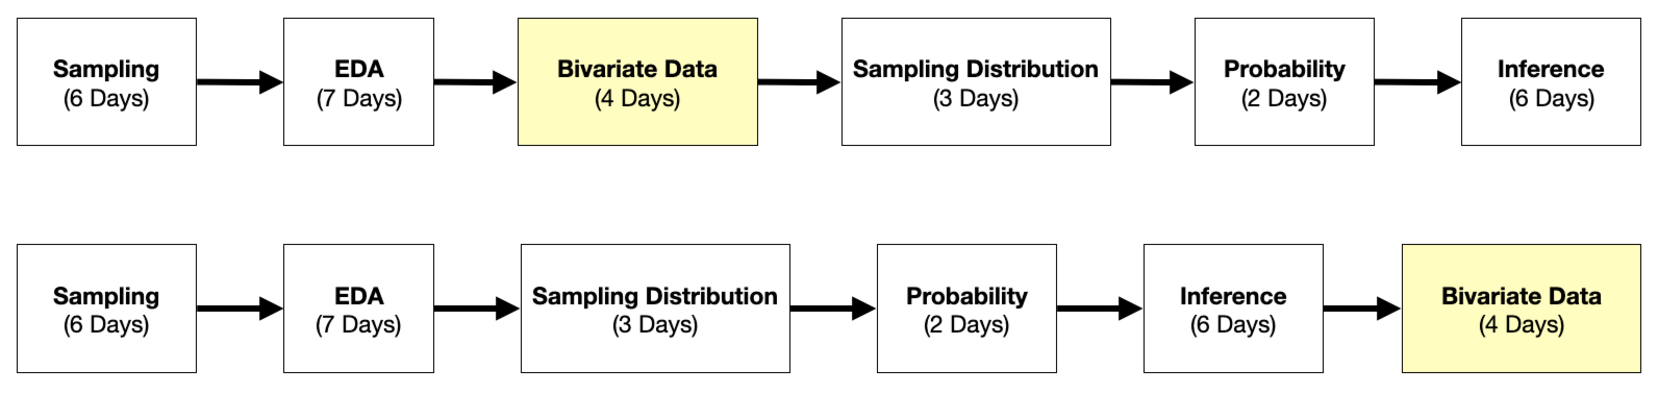
\includegraphics[width=1\linewidth]{figure/fig-03-01} 

}

\caption[The two sequences taught during Fall semester 2005]{The two sequences taught during Fall semester 2005. The unit on bivariate data is highlighted.}\label{fig:fig-3-1}
\end{figure}

To examine if changes in students' reasoning about the foundational concepts of distribution were associated with changes in the development of students' reasoning about bivariate data, students were also assessed on their distributional reasoning four times during the course of the semester. Students were also measured on several other factors (prior algebra and statistical knowledge, and general knowledge). These measures were examined as potential covariates to help explain the pattern in students' development of reasoning about bivariate data.

\hypertarget{subjectssetting}{%
\section{Subjects/Setting}\label{subjectssetting}}

The study participants consisted of \(n=113\) undergraduate students, each enrolled in one of four sections of a non-calculus based, introductory statistics course in the Educational Psychology department at the University of Minnesota during Fall Semester 2005. These students were typically female social science majors (84\% females and 16\% males) who were enrolled in the course to complete part of their major requirements. The students enrolled in the course during the study seemed representative of the students who typically take the course. These students belong to the larger population of undergraduate social science majors who take an introductory statistics course in an Educational Psychology department.

This particular introductory statistics course was designed so that it was aligned with recent \emph{Guidelines for the Assessment and Instruction in Statistics Education} endorsed by the American Statistical Association (\protect\hyperlink{ref-asa:2005a}{American Statistical Association, 2005b}). These guidelines consist of the following six recommendations (\protect\hyperlink{ref-asa:2005}{American Statistical Association, 2005a}):

\begin{enumerate}
\def\labelenumi{\arabic{enumi}.}
\tightlist
\item
  Emphasize statistical literacy and develop statistical thinking.
\item
  Use real data.
\item
  Stress conceptual understanding rather than mere knowledge of procedures.
\item
  Foster active learning in the classroom.
\item
  Use technology for developing concepts and analyzing data.
\item
  Use assessments to improve and evaluate student learning.
\end{enumerate}

In addition, the course materials were based on what has been learned from research literature on teaching and learning statistics. The research guided both the structure of the course (i.e., scope and sequence) and the instructional methods (i.e., activities, technologies, and discussions) used within the course. The course includes collecting and analyzing real data sets, software programs to illustrate abstract concepts, and many active learning techniques. Lesson plans for every instructional session were created during the initial design phase of the course in the summer of 2004, which included class goals, discussion questions and a sequence of activities. These lesson plans provide more consistency across multiple sections of the course taught by different instructors. These materials were used, evaluated and revised during two semesters before the beginning of the current study in Fall Semester 2005.

There were four sections of the course taught by two different instructors who followed identical lesson plans throughout the duration of the course and met regularly to help ensure consistency between the sections. Both of the instructors had helped develop the course materials and had taught the course multiple times prior to the time of this study. Both instructors were experienced teachers, having both high school and college teaching experience, and were doctoral students in the Quantitative Methods in Education (QME) program with a concentration in Statistics Education, so they were familiar with the current guidelines and relevant research.

\hypertarget{instruments}{%
\section{Instruments}\label{instruments}}

To help determine what covariates might be important in explaining the pattern of students' development of reasoning about bivariate data, students were assessed on several factors in addition to their reasoning about both univariate distribution and bivariate data. These included prior mathematical and statistical knowledge, as well as prior coursework in mathematics, statistics and computer science. Several different instruments were used. Each of these instruments is described in this section, and included in \protect\hyperlink{appendix-a}{Appendix A}.

The instruments that were used in this study will be described in two groups. The first group contains instruments that provided measures of students' statistical reasoning. Measures were needed to assess both reasoning about bivariate data and univariate distributions (see \protect\hyperlink{assess-statreason}{Section 3.3.1}). The instruments used, the Bivariate Reasoning Assessment (BRA), the Comprehensive Assessment of Outcomes in a First Statistics course (CAOS), and the Distributional Reasoning Scale (DRS), were developed by the NSF-Funded ARTIST project. The authors of these instruments, Garfield and Chance (\protect\hyperlink{ref-garfield:2000}{2000}), defined statistical reasoning, as:

\begin{quote}
``the way people reason with statistical ideas and make sense of statistical information. This involves making interpretations based on sets of data, representations of data, or statistical summaries of data. Students need to be able to combine ideas about data and chance, which leads to making inferences and interpreting statistical results. Underlying this reasoning is a conceptual understanding of important ideas, such as distribution, center, spread, association, uncertainty, randomness, and sampling'' (p.~101).
\end{quote}

The second group of instruments measured student covariates that might explain the pattern of change in students' reasoning about bivariate data, and also serve as controls when comparing the four sections of the course. This group of instruments includes an Algebra Test, a Mathematics Background Questionnaire, the ACT, and a student survey. These instruments are described in \protect\hyperlink{assess-covar}{Section 3.3.2}. Lastly, a reliability analysis for the sample scores and responses used in this study is provided in \protect\hyperlink{reliability}{Section 3.3.3}.

\hypertarget{assess-statreason}{%
\subsection{Group 1: Assessments of Statistical Reasoning}\label{assess-statreason}}

\textbf{Bivariate Reasoning Assessment (BRA).} To measure change in students' reasoning about bivariate data, the quantitative bivariate data scale from the \emph{Assessment Resource Tools for Improving Statistical Thinking} (ARTIST; \protect\hyperlink{ref-garfield:nd}{Garfield et al., n.d.}) was administered four times during the semester. This scale consists of eight multiple-choice items designed to assess reasoning about concepts that typically appear in a unit on bivariate data in an introductory statistics course, such as correlation and regression. Content validity of the scale was determined by expert raters who all agreed the items measured the essential concepts in bivariate quantitative reasoning (\protect\hyperlink{ref-delmas:2006}{delMas et al., 2006}). Using Cronbach's Alpha, the internal consistency reliability coefficient was 0.70 based on a class test of 550 students (\protect\hyperlink{ref-delmas:2006}{delMas et al., 2006}).

\textbf{Comprehensive Assessment of Outcomes in a First Statistics Course (CAOS).} This instrument was used both to measure students' prior statistical knowledge, as well as to measure change in students' reasoning about univariate distribution. The \emph{Comprehensive Assessment of Outcomes in a First Statistics Course} (CAOS) is a forty-item test that was designed as part of the NSF-funded ARTIST project to evaluate student attainment of desired outcomes in an introductory statistics course. The 40 multiple-choice items focus on the big ideas and ``the types of reasoning, thinking and literacy skills deemed important for all students across first courses in statistics'' (\protect\hyperlink{ref-garfield:nd}{Garfield et al., n.d.}). The CAOS test has gone through an extensive development, revision, and validation process including class testing and reliability analyses. In a class testing of over 1000 students an Alpha Coefficient was calculated to be 0.77. Eighteen expert raters provided evidence of content validity by their unanimous agreement that CAOS measures basic outcomes in statistical literacy and reasoning that are appropriate for a first course in statistics (\protect\hyperlink{ref-delmas:2006}{delMas et al., 2006}).

To measure students' prior statistical knowledge, the entire CAOS test was administered to students during the first instructional session of the semester. Ten of the CAOS items were also administered three additional times during the semester. These ten items that had been identified by experts to focus on reasoning about univariate distribution, were used to measure change in students' reasoning about univariate distribution. These ten items will be referred to as the \emph{Distributional Reasoning Scale} (DRS).

\hypertarget{assess-covar}{%
\subsection{Group 2: Assessments used as Controls and Covariates}\label{assess-covar}}

\textbf{Algebra Test.} To measure students' prior algebra knowledge, 10 released items from the \emph{2003 Trends in International Mathematics and Science Study} (TIMSS) grade-8 mathematics test were administered to students during the first instructional session of the semester. The content domain of each of these 10 items was identified on the TIMSS test blueprint as Algebra. The cognitive domain of these items varied for each item, but included domains such as ``using concepts'' and ``knowing facts and procedures'' (\protect\hyperlink{ref-iaeea:2005}{International Association for the Evaluation of Educational Achievement, 2005}). Each of the TIMSS items and exams go through an extensive validation and piloting process that has been reported in the literature (\protect\hyperlink{ref-neidorf:2004}{Neidorf \& Garden, 2004}).

\textbf{Mathematics Background Questionnaire.} To measure students' mathematical background, 15 survey items were given to students during the first instructional session of the semester. These 15 items were part of the 2005 questionnaire used to examine students' mathematical backgrounds on the grade-12 \emph{National Assessment of Educational Progress} (NAEP). The validation and testing of these items has been reported in the literature (\protect\hyperlink{ref-nagb:2003}{National Assessment Governing Board, 2003}). The response options were adapted to be more suited to university students rather than high school students. This included changing the response categories from the six originally used on the NAEP questionnaire:

\begin{itemize}
\tightlist
\item
  ``I have never taken this course'',
\item
  ``I took this course in or before Grade 8'',
\item
  ``I took this course in Grade 9'',
\item
  ``I took this course in Grade 10'',
\item
  ``I took this course in Grade 11'', and
\item
  ``I took this course in Grade 12''
\end{itemize}

to the following four response categories:

\begin{itemize}
\tightlist
\item
  ``I have never taken this course'',
\item
  ``I took this course in High School'',
\item
  ``I took this course in College'', and
\item
  ``I took this course in both High School and College.''
\end{itemize}

These four responses were coded 0, 1, 2, and 3.

\textbf{ACT Test.} Students' ACT composite scores were obtained after the completion of the semester (See \protect\hyperlink{timeline}{Section 3.4}), and used as a measure of their general knowledge. The ACT is designed to assess students' general educational development and their ability to complete college-level work. The ACT consists of four tests: English, Mathematics, Reading, and Science. The score range for each of the four tests is 1--36. The composite score, as reported by ACT, is the average of the four test scores earned during a single test administration, rounded to the nearest whole number. Validity and reliability evidence are reported in the technical manual (\protect\hyperlink{ref-act:1997}{ACT, 1997}).

\textbf{Student Survey.} Students were asked to self-report certain demographic information on a survey that was administered during the second session of the semester. This data was not intended to be used as predictors in the analysis, but rather to examine the treatments for group differences. The original student survey consisted of 26 items designed to collect student data to be examined and analyzed in the course. Four of the items from that survey were used in this study. These items were:

\begin{itemize}
\tightlist
\item
  What is your age in years?
\item
  How many credits are you registered for this semester?
\item
  How many college credits have you completed?
\item
  What is your cumulative GPA?
\end{itemize}

While the use of students' self reports can be a risky endeavor, there has been evidence in the research literature that students' self-reported data can correlate quite highly with actual records (e.g., \protect\hyperlink{ref-cassady:2001}{Cassady, 2001}). Since the survey was anonymous, students were not linked to their responses on these queries. This was also thought to increase the level of honesty in responses.

\hypertarget{reliability}{%
\subsection{Reliability Analysis of Research Instruments}\label{reliability}}

A reliability analysis was conducted for the scores and responses on some of the instruments described in the previous three sections. Coefficient alpha (\protect\hyperlink{ref-cronbach:1951}{Cronbach, 1951}) was used as a measure of reliability. Cronbach's alpha coefficient for each of the sample scores for both the BRA and DRS at all four time points are reported in \ref{tab:tab-3-1}. In addition, because of the heterogeneity in observed variance, especially in the first wave, the original computed alphas were adjusted in such a way that score variance for each of the four waves would be equalized, based on the median score variance (\protect\hyperlink{ref-gulliksen:1987}{Gulliksen, 1987}). Hereafter, this value is referred to as the adjusted coefficient alpha. The equation for adjusted coefficient alpha is given in \ref{tab:tab-3-1}, and the values for this adjustment at each wave are also reported in \autoref{eq:rel-adj}.

\begin{equation}\label{eq:rel-adj}
r_{\mathrm{adj}} = 1 - \frac{S_x^2(1-r_{xx})}{S^2_{\mathrm{Med}}}
\end{equation}

where \(S_x^2\) is the original score variance, \(r_{xx}\) is the original computed reliability, and \(S^2_{\mathrm{Med}}\) is the median score variance for all the waves. Coefficient alpha was also computed for the sample scores on the CAOS and the algebra test. These are also reported in \ref{tab:tab-3-1}.

\begin{table}[H]

\caption{\label{tab:tab-3-1}Coefficient alpha for the sample scores and responses used in the study. Adjusted coefficient alpha is also displayed for the repeated measures.}
\centering
\fontsize{10}{12}\selectfont
\begin{tabu} to \linewidth {>{\raggedright\arraybackslash}p{1.75in}>{\centering}X>{\centering}X>{\centering}X>{\centering}X}
\toprule
\multicolumn{1}{c}{Assessment} & \multicolumn{1}{c}{Wave 1} & \multicolumn{1}{c}{Wave 2} & \multicolumn{1}{c}{Wave 3} & \multicolumn{1}{c}{Wave 4}\\
\midrule
\addlinespace[0.3em]
\multicolumn{5}{l}{\textbf{BRA}}\\
\hspace{1em}Coefficient alpha & 0.67 & 0.73 & 0.74 & 0.72\\
\hspace{1em}Adjusted coefficient alpha & 0.83 & 0.73 & 0.73 & 0.72\\
\hspace{1em}N & 111 & 108 & 98 & \vphantom{1} 98\\
\addlinespace[0.3em]
\multicolumn{5}{l}{\textbf{DRS}}\\
\hspace{1em}Coefficient alpha & 0.53 & 0.71 & 0.66 & 0.76\\
\hspace{1em}Adjusted coefficient alpha & 0.71 & 0.67 & 0.68 & 0.74\\
\hspace{1em}N & 111 & 108 & 98 & 98\\
\addlinespace[0.3em]
\multicolumn{5}{l}{\textbf{CAOS}}\\
\hspace{1em}Coefficient alpha & 0.81 & --- & --- & ---\\
\hspace{1em}N & 110 & --- & --- & \vphantom{1} ---\\
\addlinespace[0.3em]
\multicolumn{5}{l}{\textbf{Algebra test}}\\
\hspace{1em}Coefficient alpha & 0.64 & --- & --- & ---\\
\hspace{1em}N & 110 & --- & --- & ---\\
\bottomrule
\end{tabu}
\end{table}

\hypertarget{timeline}{%
\section{Timeline for Instrument Administration}\label{timeline}}

Each of the instruments from the previous section (except ACT and the student survey) was administered on the first day of class (Session 1) to obtain baseline measures. The BRA and DRS were also administered during three other class periods (Session 14, Session 25 and Session 29). The assessment was administered Session 14 and Session 25 because those were the two classroom sessions that immediately preceded instruction of bivariate data for each of the two course sequences listed in \ref{fig:fig-3-1}. The assessment was also given during the last classroom session of the semester (Session 29). These instruments were all administered during class time to ensure test security and integrity. (See \ref{tab:tab-3-2} for the administration schedule for all the instruments.)

\begin{table}[H]

\caption{\label{tab:tab-3-2}Assessments dministered at each of the four waves.}
\centering
\fontsize{10}{12}\selectfont
\begin{tabu} to \linewidth {>{\raggedright}X>{\raggedright}X>{\raggedright}X>{\raggedright}X}
\toprule
\multicolumn{1}{c}{Wave 1 (Session 1)} & \multicolumn{1}{c}{Wave 2 (Session 14)} & \multicolumn{1}{c}{Wave 3 (Session 25)} & \multicolumn{1}{c}{Wave 4 (Session 29)}\\
\midrule
BRA & BRA & BRA & BRA\\
DRS & DRS & DRS & DRS\\
CAOS &  &  & \\
Algebra Test &  &  & \\
Mathematics Background Questionnaire &  &  & \\
\addlinespace
Student Survey &  &  & \\
\bottomrule
\end{tabu}
\end{table}

The items from the BRA and DRS were combined into one comprehensive instrument to ease the actual administration. The items were randomized for each of the four administrations. Because of the difficulty associated with assessing students multiple times without feedback, students were offered extra credit to participate in the study (see \protect\hyperlink{appendix-b}{Appendix B}).

Student ACT scores were obtained from the Institute of Research and Reporting after the semester had been completed. To meet Institutional Review Board stipulations, students were required to fill out a separate consent form (see \protect\hyperlink{appendix-b}{Appendix B}), and return it to the researcher after grades for the course had been posted. Because of this process, it was felt that students might not be inclined to complete the consent form, which would have resulted in a fair amount of missing data. Social exchange theory was utilized in an attempt to increase the number of forms that would be completed and returned by students. Social exchange is a theory from human behavior that is used to explain the development and continuation of peoples' interactions. The theory suggests that the actions of people are motivated by the return these actions are expected to bring, and in fact usually do bring from others (e.g., \protect\hyperlink{ref-blau:1964}{Blau, 1964}). Research has generally shown that token ``incentives given along with requests to fill out a questionnaire, a form of social exchange, consistently improve response rates'' (\protect\hyperlink{ref-dillman:2000}{Dillman, 2000, p. 14}). Using this strategy, all students were given a small amount of extra credit before the completion of the semester in exchange for filling out and returning the consent form to release their ACT score. This prompted 79 of the 113 students (70\%) to return the consent form.

\hypertarget{analysis-of-data}{%
\section{Analysis of Data}\label{analysis-of-data}}

The analyses and results (see \protect\hyperlink{results}{Chapter 4}) are split into two major parts. The first of these, the descriptive analysis, involves initially examining the data in an exploratory manner including an examination of the sample data and an assessment of the equivalence between the two instructional sequences on the different covariates that were measured (e.g., gender, mathematics background). This part of the analysis will also be used in order to help facilitate a more parsimonious model during the linear mixed-effects model (LMM) analyses.

The second part of the analysis will use LMM analyses to test hypotheses related to the three research questions. Statistical models will be fitted to the data to explore the patterns of change in students' development of reasoning about bivariate data and also to formally test which covariates (e.g.~course sequence) are important in explaining those patterns. During these analyses, covariates such as course sequence change in reasoning about distribution, and other pertinent covariates found during the descriptive analyses will be introduced into our change model to help determine if they explain differences in the patterns of change. Estimates and hypothesis tests for the level-2 fixed effects will be examined to help answer the research questions. The last section in this chapter describes the LMM methodology and details more of the LMM analyses that are specific to this study.

\hypertarget{linear-mixed-effects-models}{%
\section{Linear Mixed-Effects Models}\label{linear-mixed-effects-models}}

Researchers interested in studying change are generally interested in answering two types of questions about change (\protect\hyperlink{ref-boyle:2001}{Boyle, 2001}). The first of these questions of interest is how to ``characterize each person's pattern of change over time'', and the second asks about ``the association between predictors and the patterns of change'' (\protect\hyperlink{ref-singer:2003}{Singer \& Willett, 2003, p. 8}). While the idea of measuring change has been of interest to educational researchers for years, the methodology to accommodate this type of analysis was not readily available until the 1980s (\protect\hyperlink{ref-singer:2003}{Singer \& Willett, 2003}). It was then that a class of appropriate statistical models was developed to help examine change. These models go by a variety of names---random coefficients models, mixed-effects models, hierarchical linear models (HLM), or multilevel models are just a few. These models provide a statistical methodology that allows researchers to answer both types of questions about change.

Linear mixed-effects models (LMMs) have many advantages over traditional statistical methods such as RM-MANOVA. First, LMMs can accommodate missing data. A participant need only have one observation to be included in the analysis, under the assumption that the missing data mechanism is missing at random (MAR) (e.g., \protect\hyperlink{ref-collins:2001}{Collins et al., 2001}). A second advantage of LMMs is that they allow the number and/or timing of observations to differ for subjects. A third advantage is that LMMs allow for time-varying predictors---covariates that also change over time. Finally, a fourth advantage of the LMM is that they don't require an omnibus model that is saturated. This flexibility in model specification allows for more parsimonious models, which can lead to greater power and efficiency in estimation (\protect\hyperlink{ref-verbeke:2000}{Verbeke \& Molenberghs, 2000}).

The LMM used for this study is a multi-level regression model that incorporates two components: a level-1 linear model that describes intra-individual (within subjects) change, and a level-2 conditional model that describes systematic inter-individual (between subjects) differences in change. In the level-1 model, time is used as the independent variable for predicting individual students' baselines (starting points) and trajectories (shape or pattern of the curve) in their reasoning about bivariate data. The level-2 models allow us to determine the extent that those baselines and trajectories vary as a function of one or more covariates (i.e., other measured variables, such as ACT score, that are used to differentiate individuals). The statistical model for a LMM assuming quadratic growth is specified in \autoref{eq:lmm-level-1} and \autoref{eq:lmm-level-2} then described in more detail.

\begin{equation}\label{eq:lmm-level-1}
Y_{ij} = \pi_{0i} + \pi_{1i}(\mathrm{Time}_{ij}) + \pi_{2i}(\mathrm{Time}_{ij}^2) + \epsilon_{ij}
\end{equation}

\begin{equation}\label{eq:lmm-level-2}
\begin{split}
\pi_{0i} &= \gamma_{00} + \gamma_{01}(\mathrm{Covariate}_i) + \zeta_{0i}\\[1ex]
\pi_{1i} &= \gamma_{10} + \gamma_{11}(\mathrm{Covariate}_i) + \zeta_{1i}\\[1ex]
\pi_{2i} &= \gamma_{20} + \gamma_{21}(\mathrm{Covariate}_i) + \zeta_{2i}
\end{split}
\end{equation}

\textbf{Level-1: Modeling Within-Subject Change.} The level-1 part of the model is specified in \autoref{eq:lmm-level-1}. In this equation, \(Y_ij\) is the \emph{i}th subject's response score on the BRA at the \emph{j}th time-point. \(\mathrm{Time}_{ij}\) and \(\mathrm{Time}_{ij}^2\) are the linear and quadratic time metrics, respectively. In this study all of the subjects were measured during the same classroom sessions, so these are identical for all subjects. This, however, is not a requirement for the LMM methodology. \(\pi_{0i}\) is the \emph{i}th subject's intercept, or baseline level of reasoning about bivariate data. \(\pi_{1i}\) is the \emph{i}th subject's linear rate of change in reasoning about bivariate data, and \(\pi_{2i}\) is the \emph{i}th subject's quadratic rate of change. Finally, \(\epsilon_{ij}\) is the \emph{i}th subject's residual (level-1 residual) at the \emph{j}th time-point.

\textbf{Level-2: Modeling Between-Subject Change.} The level-2 parts of the LMM are specified in \autoref{eq:lmm-level-2}. Each of these equations describes how either a students' baseline \(\pi_{0i}\) or change trajectories (\(\pi_{1i}\) and \(\pi_{2i}\)) vary as a function of one or more individual predictors or covariates. These equations all utilize only one individual predictor (\(\mathrm{Covariate}_i\)). These equations could also be extended to include many more predictors. Since the parameters from each of the level-2 equations have similar interpretations, only the first will be examined here.

\(\gamma_{00}\) is the intercept in the first level-2 equation, and would indicate the predicted value of students' baseline reasoning (\(\pi_{0i}\)) when all of the individual predictors in the model are equal to zero. \(\gamma_{01}\) represents the strength of association between \(\mathrm{Covariate}_i\) (e.g., an individual's ACT score) and their baseline level of reasoning about bivariate data (\(\pi_{0i}\)). If, for example, \(\gamma_{01}\) is positive, then higher scores or levels on the covariate tend to be associated with higher levels of reasoning about bivariate data. Lastly, \(\zeta_{0i}\) is the level-2 error term, which indicates the deviation of the \emph{i}th subject from the group.

The composite LMM is the single equation obtained by substituting the level-2 parameters into the level-1 model. The composite LMM based on \autoref{eq:lmm-level-1} and \autoref{eq:lmm-level-2} is specified in \autoref{eq:lmm-composite}.

\begin{equation}\label{eq:lmm-composite}
\begin{split}
Y_{ij} = &\bigg[\gamma_{00} + \gamma_{01}(\mathrm{Covariate}_i) + \zeta_{0i}\bigg] + \bigg[\gamma_{10} + \gamma_{11}(\mathrm{Covariate}_i) +\\
&\zeta_{1i}\bigg](\mathrm{Time}_{ij}) + \bigg[\gamma_{20} + \gamma_{21}(\mathrm{Covariate}_i) + \zeta_{2i}\bigg](\mathrm{Time}_{ij}^2) + \epsilon_{ij}
\end{split}
\end{equation}

The LMM essentially boils down to one big regression equation, where individuals' intercepts, linear rates of change, and quadratic rates of change are a function of their level or score on a covariate. The residual term in \autoref{eq:lmm-composite} indexes the deviation (or variation) from the fixed-effects (i.e., deviation from the mean change curve). This variation can be partitioned into two components: Random-effects (represented by the \(\zeta_i\) terms), and measurement error (represented by \(\epsilon_{ij}\)).

\hypertarget{hypothesis-tests-for-research-question-1}{%
\subsection{Hypothesis Tests for Research Question 1}\label{hypothesis-tests-for-research-question-1}}

In the level-1 model, the fixed-effects determine the baseline and shape of the change trajectories for individuals. We are interested in finding out what that pattern looks like. To determine what that change looks like, hypothesis tests will be run on the fixed-effects. The null hypotheses for the level-1 coefficients are:

\[
H_0: \begin{bmatrix}\pi_{0i} \\ \pi_{1i} \\ \pi_{2i}\end{bmatrix} = \mathbf{0}
\]

Using Full Maximum Likelihood (ML) estimation, the fixed-effects can also be tested by performing a likelihood-ratio to compare nested models. For each model a deviance statistic is computed, where \(\mathrm{Deviance}=-2\ln(\mathrm{Likelihood})\), and then the difference of the two deviances is compared to a chi-square distribution with degrees of freedom equal to the difference in the number of estimated parameters between the two models. Rejecting the null-hypothesis provides evidence that the more ``complex'' model should be retained. The null-hypothesis associated with these tests is that the reduced model fits equally well as the full, or more complex, model.

To decide whether level-1 coefficients should be specified as fixed, random or non-randomly varying, the variance components for the \(\pi_i\)s will be examined and tested. To ask whether random variation exists, we test the null hypotheses:

\[
H_0: \sigma^2(\pi_{qi}) = 0
\]
If the hypothesis is rejected, the coefficient will be retained as randomly varying in the model.

While the tests for random variation may provide insight into the specification of the model, the tests for random variation tend to be valid only for large sample sizes. Because of the smaller sample size used in this study, the likelihood-ratio test will again be used to help specify the model, but this time employing Restricted Maximum Likelihood (REML) estimation. This procedure will also be used to test competing covariance structures for the residuals.

\hypertarget{hypothesis-tests-for-research-questions-2-and-3}{%
\subsection{Hypothesis Tests for Research Questions 2 and 3}\label{hypothesis-tests-for-research-questions-2-and-3}}

To examine whether or not sequence and reasoning about distribution explain the pattern of change in students' reasoning about bivariate data the \(\gamma\)s from the level-2 equations will be tested. The omnibus null-hypothesis that will be tested is that there is no covariate (sequence or reasoning about distribution) interaction with the intercept, linear rate of change, or quadratic rate of change. In other words, that there are no effects due to the covariate of any type. This null hypothesis for the level-2 fixed effects can be stated as:

\[
H_0: \gamma_{01} = \gamma_{11} = \gamma_{21} = 0
\]

If the omnibus null hypothesis is rejected, then specific hypothesis tests for each of the fixed effects will be conducted. Each of the hypotheses in this study will be tested at the \(\alpha=.05\) level. These analyses should provide answers for the research questions under study. The results for these analyses are described in the next chapter.

\hypertarget{results}{%
\chapter{Results}\label{results}}

This chapter will present the quantitative results of the study. The data analysis contains three major sections. The first is a descriptive analysis which will be used to help describe the students who were enrolled in the course and also to examine differences between the two instructional sequences. This part of the data analysis will also lend guidance in choosing relevant predictors that might help explain the patterns of change in students' reasoning about bivariate data. The second part of the analysis uses a repeated-measures multivariate analysis of variance (RM-MANOVA) to examine students' change in reasoning about univariate distribution, and then uses the results of that analysis to help define student summary predictors for use in the third part of the analysis. Finally, this third part of the analysis examines both the patterns of change in students' reasoning about bivariate data and the covariates that explain that change using linear mixed-effects models (LMM).

\hypertarget{examining-the-instructional-sequences}{%
\section{Examining the Instructional Sequences}\label{examining-the-instructional-sequences}}

The two sequences (treatments) of the course need to be examined to determine if they are similar in terms of student makeup. This examination will show how successful the randomization process was, as well as help identify any predictors that might be necessary to include in later analyses. Students self reported demographic information on the first day of the course. \ref{tab:compare-seq-demo} suggests that the students in the two sequences of the course are similar on these demographic characteristics.

\begin{table}[H]

\caption{\label{tab:compare-seq-demo}Means, standard deviations, and sample sizes for demographic factors for the two instructional sequences. The sequence labeled 'Bivariate data' is the first sequence shown in Figure 3.1 and the sequence labeled 'Inference' is the second sequence in that figure. Independent samples $t$-tests are also presented.}
\centering
\fontsize{10}{12}\selectfont
\begin{tabu} to \linewidth {>{\raggedright\arraybackslash}p{1in}>{\centering}X>{\centering}X>{\centering}X}
\toprule
\multicolumn{1}{c}{Factor} & \multicolumn{1}{c}{Bivariate data} & \multicolumn{1}{c}{Inference} & \multicolumn{1}{c}{}\\
\midrule
\addlinespace[0.3em]
\multicolumn{4}{l}{\textbf{Age}}\\
\hspace{1em}$M$ & 21.87 & 21.93 & \\
\hspace{1em}$SD$ & 4.62 & 4.43 & $t(111)=-0.07,~p=0.94$\\
\hspace{1em}$N$ & 54.00 & 59.00 \vphantom{1} & \\
\addlinespace[0.3em]
\multicolumn{4}{l}{\textbf{Enrolled credits (Fall 2005)}}\\
\hspace{1em}$M$ & 15.26 & 15.54 & \\
\hspace{1em}$SD$ & 3.21 & 2.25 & $t(94.10)=-0.54,~p=0.59$\\
\hspace{1em}$N$ & 54.00 & 59.00 & \\
\addlinespace[0.3em]
\multicolumn{4}{l}{\textbf{Cumulative earned credits}}\\
\hspace{1em}$M$ & 80.93 & 70.88 & \\
\hspace{1em}$SD$ & 46.61 & 30.57 & $t(89.98)=1.31,~p=0.19$\\
\hspace{1em}$N$ & 53.00 & 52.00 & \\
\addlinespace[0.3em]
\multicolumn{4}{l}{\textbf{Cumulative GPA (4-pt scale)}}\\
\hspace{1em}$M$ & 3.24 & 3.13 & \\
\hspace{1em}$SD$ & 0.47 & 0.37 & $t(108)=1.12,~p=0.26$\\
\hspace{1em}$N$ & 53.00 & 57.00 & \\
\bottomrule
\end{tabu}
\end{table}

Summary information on these variables for all 113 students used in the study appear in \ref{tab:summary-demo-cov}. The students seem to be of a similar age and collegiate status, namely juniors (accumulated 61 to 90 credits) and full-time students (enrolled with 13 or more credits). The grade point averages (GPA) also seem comparable between the two treatments. Significance testing was also utilized for a more comprehensive comparison of the two treatments on these factors.

An \emph{F}-test to compare variances was performed on each of the demographic characteristics in \ref{tab:compare-seq-demo} to test the assumption of homogeneity of variance between the two sequences. The results of these tests (not presented) suggested that the variances were not equal between sequences for the number of semester credits students were taking and the number of cumulative credits that students had already taken. Because of the unequal variances on these two factors, \emph{t}-tests using Welch's modification to the degrees of freedom were performed to test whether these student demographics were significantly different. The two sequences were also examined for differences in average age and cumulative grade point average of the students, albeit with a traditional two-sample \emph{t}-test. The results of these tests are also presented in \ref{tab:compare-seq-demo}. These results suggest that the students in the two sequences were similar in age, were taking a similar number of credits during fall semester 2005, had a similar number of cumulative credits, and also had a similar cumulative grade point average.

The two treatments were also examined for differences in numbers of males and females. Chi-square analyses were run to examine differences between sequences. Due to the low number of males in each section, a simulated \emph{p}-value was computed for a Monte Carlo test of \(10,000\) replicates for each analysis. This analysis suggested that the two sequences were composed of similar numbers of males and females, \(\chi^2(1) = 3.44,~ p = 0.07\). The two sequences were also examined for
differences in the number of prior mathematics, statistics and computer programming courses students had taken in both high-school and college. These were self-reported on the mathematics survey that was given to the first day of class. Chi-squares were run for each item on the survey to examine differences between the sections.

\begin{landscape}
\begingroup\fontsize{10}{12}\selectfont
\begin{table}[ht]
\caption{\label{tab:summary-demo-cov}Means (standard deviations), sample sizes, and correlations for each of the demographic factors and potential covariates. Pairwise deletion was used to compute all correlations. Spearman Correlations are given in parentheses.}
\centering
\fontsize{10}{12}\selectfont
\begin{tabular}{p{1.5in}P{0.4in}P{0.4in}P{0.4in}P{1in}P{1in}P{1in}P{1in}}
\toprule
& & & & \multicolumn{4}{c}{\textbf{Correlations}} \\[1ex] \cline{4-7}
\thead{Demographic Factor} & \thead{\textit{N}} & \thead{\textit{M}} & \thead{\textit{SD}} & \thead{1.} & \thead{2.} & \thead{3.} & \thead{4.}\\
\midrule
1. Age & 113 & 21.90 & 4.50 & --- & & & \\[1ex]
2. Credits (F2005) & 113 & 15.41 & 2.74 & $-0.54~(-0.24)$ & --- & & \\[1ex]
3. Cumulative credits & 105 & 75.96 & 39.61 & $0.67~(0.77)$ & $-0.47~(-0.20)$ & --- & \\[1ex]
4. Cumulative GPA & 108 & 3.16 & 0.45 & $-0.14~(-0.30)$ & $-0.03~(0.04)$ & $0.04~(-0.08)$ & --- \\[1ex]
5. Gender & \multicolumn{7}{l}{Females: 95, Males: 18} \\[1ex]
\midrule
\addlinespace[1em]
& & & & \multicolumn{4}{c}{\textbf{Correlations}} \\[1ex] \cline{4-7}
\thead{Potential Covariate} & \thead{\textit{N}} & \thead{\textit{M}} & \thead{\textit{SD}} & \thead{6.} & \thead{7.} & \thead{8.} & \\
\midrule
6. CAOS & 111 & 5.74 & 3.62 & --- & & & \\[1ex]
7. Algebra test & 110 & 7.88 & 2.50 & $0.07~(0.09)$ & --- & & \\[1ex]
8. ACT & 70 & 23.99 & 2.84 & $0.05~(0.01)$ & $0.42~(0.37)$ & --- & \\[1ex]
\bottomrule
\end{tabular}
\end{table}
\endgroup
\end{landscape}

\noindent Due to the low counts in some cells, a simulated \emph{p}-value was computed for a Monte Carlo test of \(10,000\) replicates for each analysis. Because of the high number of comparisons being made at the same significance level, a Bonferroni adjustment was used to adjust the significance level to \(p = 0.003\). The results of these analyses are reported in \ref{tab:chi-sq}. These analyses suggest that the two sequences were composed of students with similar backgrounds in mathematics, statistics and computer science.

\begingroup\fontsize{10}{12}\selectfont
\setlength{\LTleft}{0pt}
\begin{longtable}[t]{>{\raggedright\arraybackslash}p{3in}>{\centering\arraybackslash}p{0.5in}>{\centering\arraybackslash}p{0.5in}>{\centering\arraybackslash}p{0.5in}>{\centering\arraybackslash}p{0.5in}}
\caption{\label{tab:chi-sq}Chi-square tests to examine differences between sequences in mathematics, statistics and computer science backgrounds. The $p$-values are simulated based on a Monte Carlo test with $10,000$ replicates.}\\
\toprule
\thead{Factor} & \thead{$\chi^2$} & \thead{$df$} & \thead{$p$} & \thead{N}\\
\midrule
\endfirsthead
\caption[]{Chi-square tests to examine differences between sequences in mathematics, statistics and computer science backgrounds. The $p$-values are simulated based on a Monte Carlo test with $10,000$ replicates. \textit{(continued)}}\\
\toprule
\thead{Factor} & \thead{$\chi^2$} & \thead{$df$} & \thead{$p$} & \thead{N}\\
\midrule
\endhead
\bottomrule
\multicolumn{5}{r}{\textit{(Table continues on next page)}}
\endfoot
\bottomrule
\endlastfoot
Basic or general mathematics course & 2.00 & 2 & 0.37 & 112\\
Tech-prep mathematics course & 1.62 & 3 & 0.81 & 110\\
Pre-algebra course & 1.62 & 3 & 0.68 & 111\\
Algebra I course & 2.72 & 3 & 0.44 & 112\\
Geometry course & 0.04 & 1 & 1.00 & 112\\
\midrule
Algebra II course, with trigonometry & 1.23 & 3 & 0.97 & 111\\
Algebra II course, w/o trigonometry & 3.54 & 3 & 0.32 & 109\\
Trigonometry (as a separate course) & 1.89 & 3 & 0.96 & 112\\
Pre-calculus course & 2.60 & 3 & 0.47 & 113\\
Integrated mathematics course & 2.09 & 2 & 0.47 & 112\\
\midrule
Probability or statistics course & 3.43 & 3 & 0.37 & 113\\
Calculus course & 0.54 & 3 & 0.92 & 112\\
Discrete mathematics course & 1.66 & 2 & 0.41 & 111\\
Other mathematics course & 0.59 & 2 & 0.81 & 109\\
Computer programming course & 1.72 & 2 & 0.41 & 113\\*
\end{longtable}
\endgroup{}

Measures for students were also obtained on their prior algebra (Algebra Test), and statistical knowledge (CAOS), as well as their general knowledge (ACT). Means and standard deviations of these measures for the two sequences are reported in \ref{tab:compare-seq-cov}. Because the Bartlett tests suggested that the variances for each of the predictors were homogenous, a traditional two-sample \emph{t}-test was run on each measure to determine if there were differences between the sections. The results of these tests are also reported in \ref{tab:compare-seq-cov}. The non-significance of these tests suggest that the sequences seem to be composed of similar students in terms of general knowledge and both prior algebraic and statistical knowledge.

\begin{table}[H]

\caption{\label{tab:compare-seq-cov}Means, standard deviations, and sample sizes for each of three possible covariates by sequence. Independent samples $t$-tests to compare the two sequences (assuming equal variances) are also presented.}
\centering
\fontsize{10}{12}\selectfont
\begin{tabu} to \linewidth {>{\raggedright\arraybackslash}p{1in}>{\centering}X>{\centering}X>{\centering}X}
\toprule
\multicolumn{1}{c}{Measure} & \multicolumn{1}{c}{Bivariate data} & \multicolumn{1}{c}{Inference} & \multicolumn{1}{c}{}\\
\midrule
\addlinespace[0.3em]
\multicolumn{4}{l}{\textbf{CAOS}}\\
\hspace{1em}$M$ & 5.72 & 5.62 & \\
\hspace{1em}$SD$ & 3.57 & 3.32 & $t(108)=0.70,~p=0.49$\\
\hspace{1em}$N$ & 53.00 & 57.00 \vphantom{1} & \\
\addlinespace[0.3em]
\multicolumn{4}{l}{\textbf{Algebra test}}\\
\hspace{1em}$M$ & 7.40 & 8.35 & \\
\hspace{1em}$SD$ & 2.38 & 2.54 & $t(107)=-1.91,~p=0.06$\\
\hspace{1em}$N$ & 53.00 & 57.00 & \\
\addlinespace[0.3em]
\multicolumn{4}{l}{\textbf{ACT}}\\
\hspace{1em}$M$ & 23.93 & 24.03 & \\
\hspace{1em}$SD$ & 3.08 & 2.68 & $t(67)=-0.13,~p=0.89$\\
\hspace{1em}$N$ & 30.00 & 39.00 & \\
\bottomrule
\end{tabu}
\end{table}

\hypertarget{research-question-1-nature-of-students-reasoning-over-time}{%
\section{Research Question 1: Nature of Students' Reasoning over Time}\label{research-question-1-nature-of-students-reasoning-over-time}}

To explore students' change in development in reasoning about bivariate data, a LMM was fitted to the data to help describe the pattern of change exhibited in the data. As explained in \protect\hyperlink{methods}{Chapter 3}, linear mixed-effects models provide a powerful tool for analyzing grouped data. An important piece of the mixed-effects model methodology is the correct specification of the model including both the fixed and random effects, as well as the within-group covariance structure. This is done by first using graphs and sample statistics to help provide guidance, and then more formally by computing and comparing model estimates and fit statistics to help determine the appropriate structure of the level-1 model. Before we can fit a LMM to the data, however, it is important to check the assumption that any missing data are, at worst, \emph{missing at random} (\protect\hyperlink{ref-little:1995}{Little, 1995}).

\begin{table}[H]

\caption{\label{tab:bra-by-wave}Sample sizes, and correlations on the bivariate reasoning assessment across the four waves for all cases. Spearman Correlations are given in parentheses. Means (standard deviations) are presented in bold along the diagonal.}
\centering
\fontsize{10}{12}\selectfont
\begin{tabu} to \linewidth {>{\raggedright\arraybackslash}p{1in}>{\centering}X>{\centering}X>{\centering}X>{\centering}X>{\centering}X}
\toprule
\multicolumn{1}{c}{Wave} & \multicolumn{1}{c}{N} & \multicolumn{1}{c}{1.} & \multicolumn{1}{c}{2.} & \multicolumn{1}{c}{3.} & \multicolumn{1}{c}{4.}\\
\midrule
1. Wave 1 & 111 & \textbf{0.89 (1.13)} &  &  & \\
2. Wave 2 & 108 & $-.02$ ($-.01$) & \textbf{3.97 (1.57)} &  & \\
3. Wave 3 & 98 & .07 (.07) & .38 (.39) & \textbf{4.84 (1.58)} & \\
4. Wave 4 & 98 & $-.08$ ($-.06$) & .37 (.32) & .59 (.58) & \textbf{4.80 (1.57)}\\
\bottomrule
\end{tabu}
\end{table}

\hypertarget{missing-data-patterns}{%
\subsection{Missing Data Patterns}\label{missing-data-patterns}}

Because there are students who do not have complete data (i.e., they are missing at least one wave of data; see sample sizes in \ref{tab:bra-by-wave}) it is important to examine the pattern of the missingness. When a LMM is fit to the data, it is implicitly assumed that each student's observed records are a random sample of data from their underlying true growth trajectory (\protect\hyperlink{ref-singer:2003}{Singer \& Willett, 2003}). When students have missing data on one or more measurement occasions, the observed data may not meet that assumption, and thus the parameter estimates would be biased. However, because missingness was largely due to student absenteeism, the missing at random assumption was tenable in this study.

\hypertarget{specifying-a-functional-form}{%
\subsection{Specifying a Functional Form}\label{specifying-a-functional-form}}

As in all data analysis, it is advisable, to examine the data as a way of informing the model building process. A spaghetti plot is often a first step in examining the mean structure of longitudinal data. A spaghetti plot of a random sample of 25 students' scores on the bivariate reasoning assessment (BRA) is shown in \ref{fig:spaghetti-plot}. The bend in the plot suggests that a model that incorporates both a linear and quadratic term might be included in our initial model. Examining the mean BRA scores across the four waves in Table 4.7 further substantiates this model. This seems to suggest a quick increase in the means followed by a leveling off, or maybe even some loss. This pattern is consistent with learning and forgetting curves reported in the research literature (e.g., \protect\hyperlink{ref-min:2000}{Min et al., 2000}; \protect\hyperlink{ref-murre:2006}{Murre \& Chessa, 2006}; \protect\hyperlink{ref-wozniak:1990}{Wozniak, 1990}).

\begin{figure}[H]

{\centering 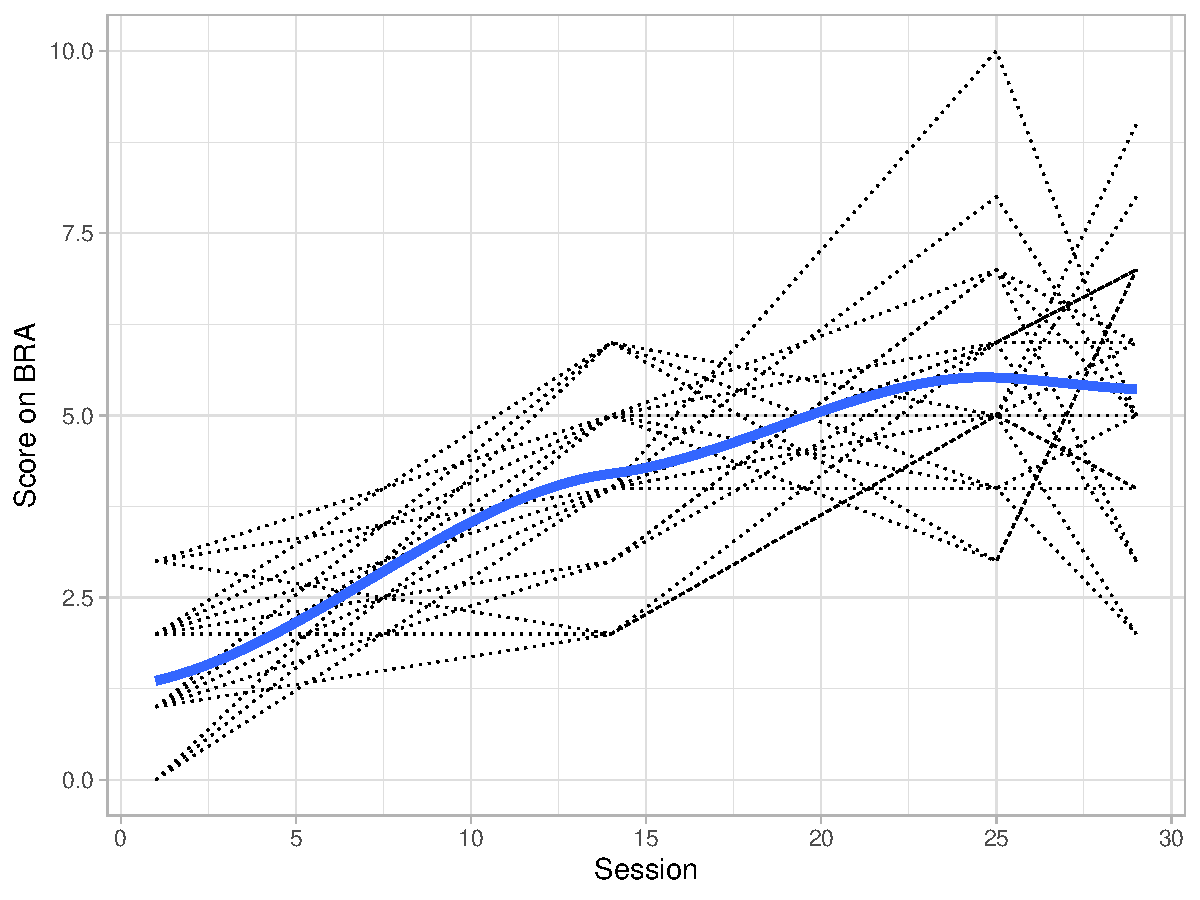
\includegraphics[width=0.8\linewidth]{thesis_files/figure-latex/spaghetti-plot-1} 

}

\caption[Spaghetti plot of BRA scores for 25 students over time]{Spaghetti plot of BRA scores for 25 students over time. The loess smoother is also displayed}\label{fig:spaghetti-plot}
\end{figure}

After settling on a functional form, the next step in the model building process is determining which parameters in the model, if any, should have random effects to help account for between-group variation. The plot in \ref{fig:spaghetti-plot} also indicates that there seems to be minor variability in the intercepts, and more variability in both the linear slopes and quadratic change between individual students. This is also seen in the standard deviations in \ref{tab:bra-by-wave}, with students exhibiting less variability in their BRA scores at the first measurement occasion then at any other measurement occasion. A linear regression of the BRA score on both day (linear) and day-squared (quadratic) was fit to the sample data, and 95-percent confidence intervals for the regression coefficients were examined to further identify the random-effects structure. These are shown in \ref{fig:ci-param}. The overlap of those intervals further substantiated that there may be no need to account for subject-to-subject variability, especially in the intercept. This will be tested more formally later in the analysis.

\begin{figure}[H]

{\centering 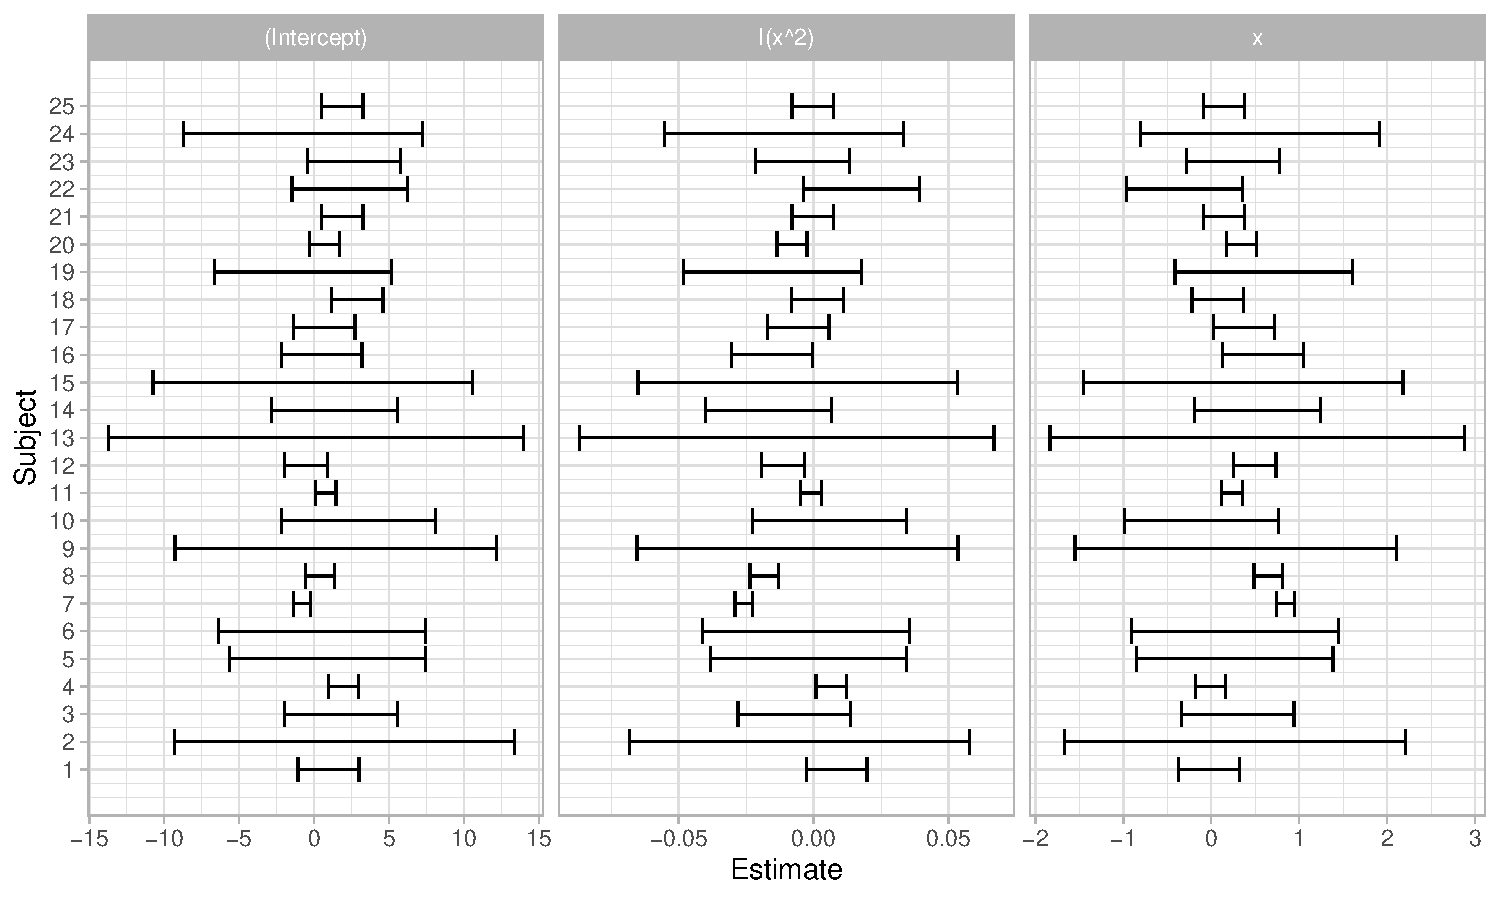
\includegraphics[width=1\linewidth]{thesis_files/figure-latex/ci-param-1} 

}

\caption[Ninety-five percent confidence intervals for the intercept, linear slope, and quadratic parameters for the 25 randomly selected students]{Ninety-five percent confidence intervals for the intercept, linear slope, and quadratic parameters for the 25 randomly selected students.}\label{fig:ci-param}
\end{figure}

\hypertarget{fitting-the-unconditional-model}{%
\subsection{Fitting the Unconditional Model}\label{fitting-the-unconditional-model}}

Applied researchers in education are generally interested in growth, or mean change across time. The unconditional model can be used to model that mean change. In an unconditional model, no predictor variables are specified (\protect\hyperlink{ref-raudenbush:2002}{Raudenbush \& Bryk, 2002}). Since this is an exploratory analysis, the goal is to find a model with both a good statistical fit to the data, and, more importantly, one that makes sense theoretically. \ref{fig:spaghetti-plot} and \ref{tab:bra-by-wave} both point to a model that incorporates an intercept, linear term, and quadratic term to describe the mean change in students' reasoning about bivariate data. The standard deviations in \ref{tab:bra-by-wave} and the confidence intervals in \ref{fig:ci-param} suggest that random effects might only be necessary for the linear and quadratic terms.

While the exploratory analyses have suggested a model that seems like a good fit to the data, in the tradition of mixed-effects models analysis, it is typical to initially fit a full mixed-effects model, with all terms having random effects at the student level. Then, competing models can be fit to the data and compared using statistical criteria. In mixed-effects model analysis three common criteria for comparing model fit are: (1) the \emph{deviance} (\(\mathrm{Deviance}=-2\ln(\mathrm{Lik.}\)), (2) the \emph{Akaike Information Criterion} (AIC; \protect\hyperlink{ref-akaike:1974}{Akaike, 1974}), and (3) the \emph{Bayesian Information Criterion} (BIC; \protect\hyperlink{ref-schwarz:1978}{Schwarz, 1978}). The deviance is used to compare nested models. The difference between the deviance for a full and reduced model is called the \emph{deviance statistic}, and is asymptotically distributed as \(\chi^2\) with degrees of freedom equal to the difference in the number of model parameters between the two models. Non-significance is evidence that the reduced, or more parsimonious model fits the data equally well.

AIC and BIC can also be used to compare the relative fit of two models. These two criteria, like the deviance statistic, are based on the log-likelihood, but penalize (i.e.~decrease) the log-likelihood according to differing criteria. The AIC penalizes according to the number of model parameters, while the BIC penalizes according to both the number of model parameters and the sample size. The AIC and BIC can be compared for any pair of models and do not require these models to be nested, with the caveat that the models are fit to an identical set of data. Because of the parameterization of these fit statistics, smaller values of AIC and BIC indicate better model fit.

To substantiate that a quadratic model is necessary to model the mean change in students' reasoning about bivariate data, three competing full mixed-effects models were fit to the data. These included a model for no change, or an intercept only model (Model A), a model for linear change (Model B), and a model for quadratic change (Model C). Each of these unconditional models was fitted using maximum likelihood (ML). All of the statistical analyses were conducted using the \texttt{\{lme4\}} (\protect\hyperlink{ref-bates:2005}{Bates \& Sarkar, 2005}) and \texttt{\{nlme\}} (\protect\hyperlink{ref-pinheiro:2005}{Pinheiro et al., 2005}) libraries in the software package R version 2.2.1 (\protect\hyperlink{ref-r-dev:2005}{R Development Core Team, 2005}). The results of these analyses are reported in \ref{tab:taxonomy-uncond}. (\emph{Note:} A cubic model for change, or saturated model, was also fit to the data, but was not reported due to problems with convergence.)

\begingroup\fontsize{10}{12}\selectfont
\begin{table}[ht]
\caption{\label{tab:taxonomy-uncond}Taxonomy of models fitted to compare potential change trajectories for the BRA ($n=113$).}
\centering
\fontsize{10}{12}\selectfont
\begin{tabular}{p{2in}P{0.75in}P{0.75in}P{0.75in}P{0.75in}}
\toprule
\thead{Effects} & \thead{Parameter} & \thead{Model A} & \thead{Model B} & \thead{Model C}\\
\midrule
\multicolumn{5}{l}{\textbf{Fixed effects}} \\[1ex]
Intercept & $\gamma_{00}$ & 3.55$^{***}$ & 1.32$^{***}$ & 0.90$^{***}$\\[1ex]
Session & $\gamma_{10}$ &  & 0.15$^{***}$ & 0.32$^{***}$\\[1ex]
Session$^2$ & $\gamma_{20}$ &  &  &$-0.01^{***}$ \\[1ex]
\addlinespace[0.3em]
\multicolumn{5}{l}{\textbf{Variance components}} \\[1ex]
Level-1: Within student & $\sigma^2_{\epsilon}$ & 4.84 & 1.74 & 1.22\\[1ex]
Level-2: Between student &  &  &  & \\[1ex]
\hspace{1em}Var(Intercept) & $\sigma^2_{0}$ & 0.00 & 0.01 & 0.04\\[1ex]
\hspace{1em}Var(Linear term) & $\sigma^2_{1}$ &  & 0.00 & 0.01\\[1ex]
\hspace{1em}Var(Quadratic term) & $\sigma^2_{2}$ &  &  & 0.00\\[1ex]
\hspace{1em}Cov(Intercept, Linear) & $\sigma_{01}$ &  & 0.00 & 0.00\\[1ex]
\hspace{1em}Cov(Intercept, Quadratic) & $\sigma_{02}$ &  &  & 0.00\\[1ex]
\hspace{1em}Cov(Linear, Quadratic) & $\sigma_{12}$ &  & & 0.00\\[1ex]
\addlinespace[0.3em]
\multicolumn{5}{l}{\textbf{Goodness-of-fit}} \\[1ex]
Deviance & & 1813.8 & 1492.1 & 1408.4\\[1ex]
AIC & & 1819.8 & 1504.1 & 1428.4\\[1ex]
BIC & & 1831.8 & 1528.2 & 1468.6 \\[1ex]
\bottomrule
\multicolumn{5}{l}{\textit{Note.} Variance components with values less than 0.01 are reported as `0.00'.}\\
\multicolumn{5}{l}{$^{\sim}p<0.10,~^{*}p<0.05,~^{**}p<0.01,~^{***}p<0.001$}\\
\end{tabular}
\end{table}
\endgroup

As we consider the fixed-effects that should be included, we first examine the unconditional means model (Model A) more closely. In the unconditional means model, variation in students' reasoning about bivariate data is partitioned across students without regard to time. The results from this model will allow an exploration of whether there is systematic variation in students' reasoning that is worth exploring, and also where that variation resides (within or between students). This model will also provide baseline information to evaluate subsequent models against.

\hypertarget{model-a-the-unconditional-means-model}{%
\subsubsection*{Model A: The Unconditional Means Model}\label{model-a-the-unconditional-means-model}}
\addcontentsline{toc}{subsubsection}{Model A: The Unconditional Means Model}

The unconditional means model doesn't describe change, but rather describes and partitions the variation in students' reasoning about bivariate data. This model lacks predictors at both level-1 and level-2:

\begin{equation}\label{eq:model-a}
\begin{split}
Y_{ij} &= \pi_{0i}  + \epsilon_{ij}\\[2ex]
\pi_{0i} &= \gamma_{00} + \zeta_{0i}\\[1ex]
\end{split}
\end{equation}

where it is assumed that:

\[
\epsilon_{ij} \sim \mathcal{N}(0,\sigma^2_{\epsilon})~\mathrm{and}~\zeta_{0i} \sim \mathcal{N}(0,\sigma^2_{0})
\]

This model lacks a slope parameter and is therefore completely flat sitting at elevation \(\pi_{0i}\) for person \emph{i}. While these flat trajectories may differ in elevation for different students, the average elevation is \(\gamma_{00}\). This model postulates that the observed level of reasoning for student \emph{i} on measurement occasion \emph{j} is composed of deviations about the two means just described, namely the overall average mean and the student-specific mean.

Model A in \ref{tab:taxonomy-uncond} presents the results of fitting the unconditional means model to the bivariate reasoning data. The one fixed effect in this model (\(\hat\gamma_{00}=3.55\)) estimates the average score on the BRA for all students across all measurement occasions. Rejection of its associated null-hypothesis (\(p<0.001\)) confirms that the average score on the BRA throughout an entire introductory statistics course is non-zero.

Examining the random-effects, we see that the estimated within-student variance
(\(\hat\sigma^2_{\epsilon}\)) is 4.832. The estimated between-student variance (\(\hat\sigma^2_{0}\)) is \(1.96 \times 10^{-17}\). The hypothesis test for the within-student variance is significant (\(p < 0.001\)) and suggests that the average student's BRA score varies over time. The small between-student variance might suggest that students do not vary much in their reasoning about bivariate data from each other. Because the within-student variance component is significantly different from zero, there is a need to link that variation to other predictors.

The unconditional means model will be used as a baseline for the evaluation of models with more complex functional forms using the criteria set out earlier in this section. The smaller AIC and BIC values as well as the significant linear and quadratic fixed-effects all suggest that the quadratic model (Model C) should be adopted. Since the linear and quadratic coefficients were added in successive models after initially constraining them to zero in Model A, likelihood ratio tests can be used to compare the model fit of each lower parameter model (reduced model) to the next higher parameter model (full model). In students' reasoning about bivariate data, both the linear model---\(\chi^2(3)=321.65\), \(p < 0.001\)---and the quadratic model---\(\chi^2(4)=83.74\), \(p < 0.001\)---were significant. All of these results indicate that the quadratic model should be adopted. It is this model that is described next.

\hypertarget{model-c-the-unconditional-quadratic-change-model}{%
\subsubsection*{Model C: The Unconditional Quadratic Change Model}\label{model-c-the-unconditional-quadratic-change-model}}
\addcontentsline{toc}{subsubsection}{Model C: The Unconditional Quadratic Change Model}

Based on the exploratory analysis and the likelihood ratio tests to compare nested models, a quadratic change model was adopted (Model C). This model will partition the variation in students BRA scores across both students and time. This model is described in \autoref{eq:model-c}:

\begin{equation}\label{eq:model-c}
\begin{split}
Y_{ij} &= \pi_{0i} + \pi_{1i}(\mathrm{Session}_{ij}) + \pi_{2i}(\mathrm{Session}_{ij}^2) + \epsilon_{ij}\\[2ex]
\pi_{0i} &= \gamma_{00} + \zeta_{0i}\\[1ex]
\pi_{1i} &= \gamma_{10} + \zeta_{1i}\\[1ex]
\pi_{2i} &= \gamma_{20} + \zeta_{2i}\\[1ex]
\end{split}
\end{equation}

where we assume that:

\[
\epsilon_{ij} \sim \mathcal{N}(0,\sigma^2_{\epsilon})~\mathrm{and}~\begin{bmatrix}\zeta_{0i} \\ \zeta_{1i} \\ \zeta_{2i}\end{bmatrix} \sim \mathcal{N}\bigg(\begin{bmatrix}0 \\ 0 \\ 0\end{bmatrix},\begin{bmatrix}\sigma^2_{0} & \sigma_{01} & \sigma_{02} \\ \sigma_{10} & \sigma^2_{1} & \sigma_{12} \\ \sigma_{20} & \sigma_{21} & \sigma^2_{2}\end{bmatrix}\bigg)
\]

Because the only predictors in this model are associated with time (\(\mathrm{Session}_{ij}\) and \(\mathrm{Session}_{ij}^2\)), it is referred to as the \emph{unconditional quadratic change model}. Since we have altered the level-1 specification, this changes the meaning of both the residuals and the variance components. Now the level-1 residual indicates the deviation from that student's quadratic change trajectory. Likewise, the residual variance (\(\hat\sigma^2_{\epsilon}\)) now summarizes the scatter of each student's data around that trajectory. The level-2 residuals now summarize between-student variability in initial status, linear, and quadratic rates of change, respectively.

Model C, presented in \ref{tab:taxonomy-uncond}, shows the results of fitting an unconditional growth model to the bivariate reasoning data. The fixed-effects, \(\hat\gamma_{00}\), \(\hat\gamma_{10}\), and \(\hat\gamma_{20}\), estimate the average initial score, average linear rate of change, and average quadratic rate of change on the BRA. The null hypothesis is rejected (\(p<0.001\)) for each of these parameters, estimating that the average change in students reasoning about bivariate data as depicted by the BRA has a non-zero starting score of 0.90, a non-zero linear change of 0.33 per instructional session, and a non-zero quadratic change of \(-0.006\). This trajectory is plotted in \ref{fig:fitted-model-c}. This suggests that on average, students begin the course with very little ability to reason about bivariate data. The linear and quadratic rates of change suggest that on average this ability increases throughout an introductory statistics course, and might either plateau or drop very slightly especially in later sessions.

\begin{figure}[H]

{\centering 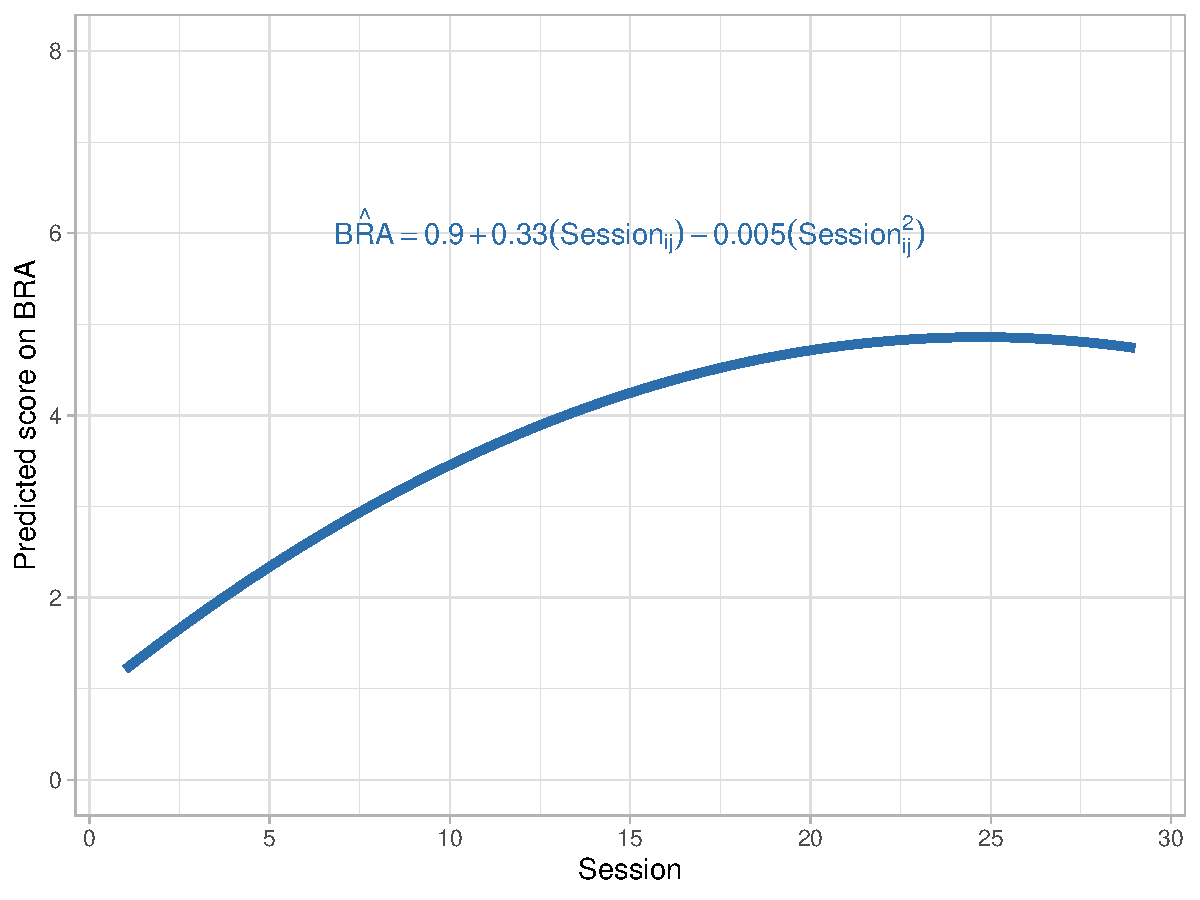
\includegraphics[width=0.8\linewidth]{thesis_files/figure-latex/fitted-model-c-1} 

}

\caption[Fitted curve for Model C showing the average predicted change in bivariate reasoning across class session]{Fitted curve for Model C showing the average predicted change in bivariate reasoning across class session.}\label{fig:fitted-model-c}
\end{figure}

The level-1 residual variance summarizes the average scatter of an individual student's observed BRA scores around his/her change trajectory. This estimated within-student variance (\(\hat\sigma^2_{\epsilon}=1.197\)) shows major reduction from the within-student variance from both Model A and Model B. Because the null hypothesis associated with this variance component was rejected (\(p<0.001\)), this suggests there is still within-student variation to account for so it may be profitable to introduce substantive predictors into future models.

The level-2 variance components quantify the amount of unpredicted variation in the individual growth parameters. The non-significance of the variance components associated with both the intercept and quadratic change parameters suggests that students may not vary in either their initial ability to reason about bivariate data or in their quadratic rate of change. The variance component for the linear rate of change is also non significant. The tests associated with these components, however, are conservative with small sample sizes. For this reason other model comparison criteria needs to be consulted before removing any random effects. Before the random-effects can be examined, it is prudent to examine the covariance structure of the residuals for proper fit.

\hypertarget{specifying-a-covariance-structure-for-the-residuals}{%
\subsection{Specifying a Covariance Structure for the Residuals}\label{specifying-a-covariance-structure-for-the-residuals}}

Efficient estimation of mean change is dependent on the adoption of an appropriate variance-covariance structure for the residuals (\protect\hyperlink{ref-diggle:1988}{Diggle, 1988}). This structure can be determined initially by using traditional multiple regression to fit the most complex model being examined (quadratic model for change; \autoref{eq:model-c}) and examining the residuals. The residuals suggest homogeneity of variance over time indicating that the variance-covariance structures that need to be examined should include a constant variance structure. Three alternative error covariance structures that have been identified as common in longitudinal analyses (\protect\hyperlink{ref-singer:2003}{Singer \& Willett, 2003}) were fitted to the data: unstructured, compound symmetric, and continuous autoregressive. Each of these models was fitted using \emph{restricted maximum likelihood} (REML). Because the models have identical fixed-effects, ML or REML could be used to compare the models. However, REML produces goodness-of-fit statistics that only reflect the fit of the models stochastic portion, which is the focus of this part of the investigation. Likelihood tests, as well as both AIC and BIC comparisons were used to select an appropriate structure for the residuals. Based on these results (see \ref{tab:error-struc}), a random-effects structure with unstructured residuals was adopted for all models to further test the random-effects.

\begin{table}[H]

\caption{\label{tab:error-struc}Selection of alternative error variance-covariance structures for use with the quadratic model for change in reasoning about bivariate data. The results of the likelihood ratio tests (LRT) are from comparison with the model that used an unstructured error variance-covariance structure.}
\centering
\fontsize{10}{12}\selectfont
\begin{tabu} to \linewidth {>{\raggedright\arraybackslash}p{1.75in}>{\centering\arraybackslash}p{0.25in}>{\centering\arraybackslash}p{0.5in}>{\centering\arraybackslash}p{0.5in}>{\centering\arraybackslash}p{0.5in}>{\centering\arraybackslash}p{1.5in}}
\toprule
\multicolumn{1}{c}{Variance Structure} & \multicolumn{1}{c}{$df$} & \multicolumn{1}{c}{Deviance} & \multicolumn{1}{c}{AIC} & \multicolumn{1}{c}{BIC} & \multicolumn{1}{c}{LRT}\\
\midrule
Unstructured & 10 & 1432.37 & 1452.38 & 1492.49 & \\
Compound Symmetry & 11 & 1432.37 & 1454.37 & 1498.49 & $\chi^2(1)=0.01,~p=0.94$\\
Continous Autoregressive & 11 & 1430.17 & 1452.17 & 1496.29 & $\chi^2(1)=2.21,~p=0.14$\\
\bottomrule
\end{tabu}
\end{table}

\hypertarget{testing-the-random-effects}{%
\subsection{Testing the Random-Effects}\label{testing-the-random-effects}}

After having specified the covariance structure of the residuals, we can now examine the random-effects to see which should be included in the model. While some programs (e.g., SAS) output \emph{p}-values for the random-effects, these are based on a \emph{z}-test and with the small sample size in this study, the results are hazy at best. However as Bates (\protect\hyperlink{ref-bates:2005a}{2005, July 13}) writes,

\begin{quote}
``(i)t is possible to do a likelihood ratio test on two fitted \ldots models with different specifications of the random effects. The \emph{p}-value for such a test is calculated using the chi-squared distribution from the asymptotic theory, which does not apply in most such comparisons because the parameter for the null hypothesis is on the boundary of the parameter region. The \emph{p}-value shown will be conservative (that is, it is an upper bound on the true \emph{p}-value).''
\end{quote}

The earlier analyses suggested that a model that didn't include random-effects on the intercept might be a good fit to the data. This model was fitted using REML and compared using a likelihood ratio test to the full unconditional model (Model C). The results of that comparison---\(\chi^2(3)=0.539,~p=0.91\)---indicated that the more parsimonious model (no random-effects associated with the intercept term) should be retained. Further testing showed that both the linear and quadratic terms needed random-effects. (These results are not presented.) The output for this model (Model D) is shown in \ref{tab:model-d}.

\begingroup\fontsize{10}{12}\selectfont
\begin{table}[ht]
\caption{\label{tab:model-d}Final unconditional model used to describe students' change in reasoning about bivariate data.}
\centering
\fontsize{10}{12}\selectfont
\begin{tabular}{p{3in}P{1in}P{1.5in}}
\toprule
\thead{Effects} & \thead{Parameter} & \thead{Model D}\\
\midrule
\multicolumn{3}{l}{\textbf{Fixed effects}} \\[1ex]
Intercept & $\gamma_{00}$ & 0.90$^{***}$\\[1ex]
Session & $\gamma_{10}$ & 0.32$^{***}$\\[1ex]
Session$^2$ & $\gamma_{20}$ &$-0.01^{***}$ \\[1ex]
\addlinespace[0.3em]
\multicolumn{3}{l}{\textbf{Variance components}} \\[1ex]
Level-1: Within student & $\sigma^2_{\epsilon}$ & $1.23^{***}$\\[1ex]
Level-2: Between student & \\[1ex]
\hspace{1em}Var(Intercept) & $\sigma^2_{0}$ & ---\\[1ex]
\hspace{1em}Var(Linear term) & $\sigma^2_{1}$ &  $0.01^{**}$\\[1ex]
\hspace{1em}Var(Quadratic term) & $\sigma^2_{2}$ &  $0.00001^{\sim}$\\[1ex]
\hspace{1em}Cov(Intercept, Linear) & $\sigma_{01}$ &---\\[1ex]
\hspace{1em}Cov(Intercept, Quadratic) & $\sigma_{02}$ & ---\\[1ex]
\hspace{1em}Cov(Linear, Quadratic) & $\sigma_{12}$ & $-0.0004^{\sim}$\\[1ex]
\addlinespace[0.3em]
\multicolumn{3}{l}{\textbf{Goodness-of-fit}} \\[1ex]
Deviance & & 1432.9\\[1ex]
AIC & & 1446.9\\[1ex]
BIC & & 1475.0 \\[1ex]
\bottomrule
\multicolumn{3}{l}{$^{\sim}p<0.10~^{*}p<0.05,~^{**}p<0.01,~^{***}p<0.001$}\\
\end{tabular}
\end{table}
\endgroup

Model D still maintains the same fixed-effects as Model C, but has different random-effects based on an examination of the variance components and tests of model comparison for a series of models that are not shown. Model D is shown in \autoref{eq:model-d}:

\begin{equation}\label{eq:model-d}
\begin{split}
Y_{ij} &= \pi_{0i} + \pi_{1i}(\mathrm{Session}_{ij}) + \pi_{2i}(\mathrm{Session}_{ij}^2) + \epsilon_{ij}\\[2ex]
\pi_{0i} &= \gamma_{00} + \zeta_{0i}\\[1ex]
\pi_{1i} &= \gamma_{10} + \zeta_{1i}\\[1ex]
\pi_{2i} &= \gamma_{20} + \zeta_{2i}\\[1ex]
\end{split}
\end{equation}

where it is assumed that:

\[
\epsilon_{ij} \sim \mathcal{N}(0,\sigma^2_{\epsilon})~\mathrm{and}~\begin{bmatrix}\zeta_{1i} \\ \zeta_{2i}\end{bmatrix} \sim \mathcal{N}\bigg(\begin{bmatrix}0 \\ 0\end{bmatrix},\begin{bmatrix}\sigma^2_{1} & \sigma_{12} \\ \sigma_{21} & \sigma^2_{2}\end{bmatrix}\bigg)
\]

The estimated fixed-effects have changed very little from Model C to Model D,
and all three remain significant (\(p<0.001\)). The within-student variance component has increased slightly, but also remains significant (\(p<0.001\)). While the estimated variance components for the linear rate of change and the quadratic rate of change have not changed much, by not allowing the intercept to vary between students, the test associated with the variance component for the linear rate of change is now non-zero (\(p<.05\)). And, while the significance test for the variance component for the quadratic rate of change is marginally significant (\(p<0.10\)) the likelihood ratio test suggested that this random-effect needed to be retained in the model. The covariance, which is also marginally significant (\(p<0.10\)), informs us of the relationship between linear rate of change and quadratic rate of change. Interpretation can be easier if the covariance is re-expressed as a correlation coefficient. This can be done by dividing the covariance by the square root of the product of its associated variance components:

\begin{equation}\label{eq:corr}
\hat\rho_{\pi_1,\pi_2} = \frac{\hat\sigma_{01}}{\sqrt{\hat\sigma_0^2\hat\sigma_1^2}} = -0.936
\end{equation}

We conclude that the relationship between the average linear rate of change and quadratic rate of change in students' ability to reason about bivariate data is both negative, strong and, since the hypothesis test is significant, is likely non-zero. This indicates that students who have higher linear rates of change also tend to have lower quadratic rates of change.

Model D suggests that students, on average, have some ability to reason about bivariate data before any instruction in an introductory statistics course as indicated by the significance of the intercept fixed-effect term. There also seems to be very little variability in students' baseline reasoning about bivariate data. In other words, they all seem to be starting at the same place. The significance of the positive linear fixed-effect term suggests that students, on average, are increasing their level of reasoning about bivariate data throughout an introductory statistics course, but this growth does not persist due to the negative quadratic fixed-effect term. Eventually, due to numeric reasons alone, the quadratic term will remove more than the linear term will add, causing the trajectory to peak and then decline. For an average student, this peak occurs around instructional session 24 in this data. Both of these rates of change vary from student-to-student. An average students' growth curve throughout an introductory statistics course (29 sessions) is depicted in \ref{fig:fitted-model-c}.

It is required that the random effects are normally distributed with a zero mean and covariance matrix \(\boldsymbol\Phi=\begin{bmatrix}\sigma^2_{1} & \sigma_{12} \\ \sigma_{21} & \sigma^2_{2}\end{bmatrix}\), and that they are independent for different groups. Furthermore, it is also assumed that the within-group errors (\(\sigma^2_{\epsilon}\)) have a zero mean and constant variance, and are independent of the random effects. Exploratory analysis on the residuals of the fitted models (not presented) revealed that the above assumptions were adequately met, according to the inspection criteria described by Pinheiro and Bates (\protect\hyperlink{ref-pinheiro:2000}{2000}).

\hypertarget{research-question-2-importance-of-instructional-sequence}{%
\section{Research Question 2: Importance of Instructional Sequence}\label{research-question-2-importance-of-instructional-sequence}}

To answer the second research question (Is the sequencing of bivariate data within a course associated with changes in the pattern of development of students' reasoning about bivariate data?), a conditional LMM will be used to help provide an answer for this research question. A conditional model, unlike the unconditional model described earlier, allows for predictors other than just time. To answer this research question, the predictor of instructional sequence will be introduced into the quadratic model for change that was adopted in the previous section (Model D). The two sequences shown in \ref{fig:fitted-model-c} will be coded \(-1\) (Bivariate data first) and \(+1\) (Inference first), respectively. The specification of the level-1 and level-2 models is presented in \autoref{eq:model-e}:

\begin{equation}\label{eq:model-e}
\begin{split}
Y_{ij} &= \pi_{0i} + \pi_{1i}(\mathrm{Session}_{ij}) + \pi_{2i}(\mathrm{Session}_{ij}^2) + \epsilon_{ij}\\[2ex]
\pi_{0i} &= \gamma_{00} + \gamma_{01}(\mathrm{Sequence}_{j}) + \zeta_{0i}\\[1ex]
\pi_{1i} &= \gamma_{10} + \gamma_{11}(\mathrm{Sequence}_{j}) + \zeta_{1i}\\[1ex]
\pi_{2i} &= \gamma_{20} + \gamma_{21}(\mathrm{Sequence}_{j}) + \zeta_{2i}\\[1ex]
\end{split}
\end{equation}

\ref{tab:model-e} shows the results from fitting a model to the bivariate reasoning data that includes instructional sequence as a predictor of initial status, linear rate of change, and quadratic rate of change (Model E).

\begingroup\fontsize{10}{12}\selectfont
\begin{table}[ht]
\caption{\label{tab:model-e}Final unconditional model used to describe students' change in reasoning about bivariate data.}
\centering
\fontsize{10}{12}\selectfont
\begin{tabular}{p{3in}P{1in}P{1.5in}}
\toprule
\thead{Effects} & \thead{Parameter} & \thead{Model E}\\
\midrule
\multicolumn{3}{l}{\textbf{Fixed effects}} \\[1ex]
Intercept & $\gamma_{00}$ & 0.90$^{***}$\\[1ex]
Instructional Sequence & $\gamma_{01}$ & $-0.07$\\[1ex]
Session & $\gamma_{10}$ & 0.32$^{***}$\\[1ex]
Instructional Sequence $\times$ Session & $\gamma_{11}$ & $-0.00004$\\[1ex]
Session$^2$ & $\gamma_{20}$ &$-0.01^{***}$ \\[1ex]
Instructional Sequence $\times$ Session$^2$ & $\gamma_{21}$ & 0.0002\\[1ex]
\addlinespace[0.3em]
\multicolumn{3}{l}{\textbf{Variance components}} \\[1ex]
Level-1: Within student & $\sigma^2_{\epsilon}$ & $1.24^{***}$\\[1ex]
Level-2: Between student & \\[1ex]
\hspace{1em}Var(Linear term) & $\sigma^2_{1}$ &  $0.01^{**}$\\[1ex]
\hspace{1em}Var(Quadratic term) & $\sigma^2_{2}$ &  $0.00001^{\sim}$\\[1ex]
\hspace{1em}Cov(Linear, Quadratic) & $\sigma_{12}$ & $-0.0004^{\sim}$\\[1ex]
\addlinespace[0.3em]
\multicolumn{3}{l}{\textbf{Goodness-of-fit}} \\[1ex]
Deviance & & 1451.7\\[1ex]
AIC & & 1471.7\\[1ex]
BIC & & 1511.9 \\[1ex]
\bottomrule
\multicolumn{3}{l}{$^{\sim}p<0.10~^{*}p<0.05,~^{**}p<0.01,~^{***}p<0.001$}\\
\end{tabular}
\end{table}
\endgroup

\hypertarget{model-e-the-uncontrolled-effects-of-instructional-sequence}{%
\subsubsection*{Model E: The Uncontrolled Effects of Instructional Sequence}\label{model-e-the-uncontrolled-effects-of-instructional-sequence}}
\addcontentsline{toc}{subsubsection}{Model E: The Uncontrolled Effects of Instructional Sequence}

Model E includes instructional sequence as a predictor of initial status, as well as both linear and quadratic change. Interpretation of its six fixed-effects is straightforward: (1) the estimated score on the BRA for all students at the beginning of an introductory statistics course is on average 0.90 (\(p<0.001\)); (2) for students enrolled in courses that taught the second instructional sequence, the baseline score is \(0.07\) points lower, on average (\(p=0.49\)); (3) the estimated average linear rate of change in BRA score for all students is 0.32 (\(p<0.001\)); (4) for students enrolled in courses that taught the second instructional sequence, the linear rate of change is 0.00004 lower, on average (\(p=0.999\)); (5) the estimated average quadratic rate of change for all students is \(-0.01\) (\(p<0.001\)); (6) and lastly, for students enrolled in courses that taught the second instructional sequence, the quadratic rate of change is 0.0002 higher, on average (\(p=0.78\)). These results suggest that on average, students in both sequences have similar development in their reasoning about bivariate data throughout an introductory statistics course. In other words, the initial differences in average BRA scores between students taking a course that utilized the first instructional sequence and students taking a course that utilized the second instructional sequence are statistically indistinguishable from zero. Likewise, the differences in average linear rate of change and average quadratic rate of change are also not distinguishable from zero.

The significant within-student variance component in Model E is virtually identical to that from Model D. This is expected since there were no level-1 predictors that were added to this model. Both of the level-2 variance components are also essentially unchanged. These conditional variances quantify the inter-individual differences in linear and quadratic change, respectively, that remain unexplained by the predictor.

Because sequence of instruction did not seem to explain any of more variation in either linear or quadratic change, it can most likely be removed from the model as an important predictor, but since instructional sequence is a focal predictor in answering our research questions, this temptation will be resisted until future models are explored.

\hypertarget{research-question-3-importance-of-foundational-concepts-of-distribution}{%
\section{Research Question 3: Importance of Foundational Concepts of Distribution}\label{research-question-3-importance-of-foundational-concepts-of-distribution}}

To answer the third research question (Are changes in students' reasoning about the foundational concepts of distribution associated with changes in the pattern of development of students' reasoning about bivariate data?), the change in students' reasoning about distribution needs to be examined and summarized. This analysis employed RM-ANOVA to examine the average within-subjects differences in students' reasoning about distribution. It will help define which time-points will be most useful in forming individual summary predictors (e.g., difference between the scores at the 1st and 4th time-point vs.~mean score) for use in a conditional LMM analysis. That analysis will then be used to test hypotheses about whether changes in students' reasoning about univariate distribution explains changes in their reasoning about bivariate data.

\hypertarget{examining-students-reasoning-about-distribution}{%
\subsection{Examining Students' Reasoning About Distribution}\label{examining-students-reasoning-about-distribution}}

Students' reasoning scores using the \emph{Distributional Reasoning Scale} (DRS) were analyzed in a multivariate analysis of variance with time of measurement (Session 1 vs.~Session 14 vs.~Session 25 vs.~Session 29) as a within-subjects factor. The main effect for time of measurement was significant, Wilk's \(\Lambda=0.059,~F(3,~80) = 425.367,~p<.001\).

Post-hoc comparisons were performed using the Bonferroni adjustment for multiple comparisons. Students' reasoning about distribution tended to increase throughout the course. Distributional reasoning scores were increased from a mean of 0.72 (\(SD=0.12\)) at the first measurement occasion to a mean of 7.42 (\(SD=0.18\), \(p<.001\)) immediately on the second measurement occasion. The improvement was maintained at both the third (\(M=7.49,~SD=0.17,~p<.001\)) and fourth (\(M=7.53,~SD=0.18,~p<.001\)) measurement occasions. There was no difference between the second measurement occasion mean and the third measurement occasion mean (\(p=1.00\)), nor between the mean score at the second measurement occasion and the fourth measurement occasion mean (\(p=1.00\)). There was also no significant difference between the third measurement occasion and the fourth (\(p=1.00\)) measurement occasion.

\hypertarget{examining-and-interpreting-the-conditional-model}{%
\subsection{Examining and Interpreting the Conditional Model}\label{examining-and-interpreting-the-conditional-model}}

Because of the results of the analyses from the previous section, difference scores between the first and last measurement occasions were used as a proxy for describing the change in students' development in reasoning about distribution. These scores were then mean centered to facilitate interpretations. These measures are used in subsequent analyses to examine if changes in students' reasoning about distribution are important in explaining changes in students' reasoning about bivariate data. A conditional LMM using these centered difference scores was run on the bivariate reasoning data. The specification of the level-1 and level-2 models for this analysis is presented in \autoref{eq:model-f}:

\begin{equation}\label{eq:model-f}
\begin{split}
Y_{ij} &= \pi_{0i} + \pi_{1i}(\mathrm{Session}_{ij}) + \pi_{2i}(\mathrm{Session}_{ij}^2) + \epsilon_{ij}\\[2ex]
\pi_{0i} &= \gamma_{00} + \gamma_{01}(\mathrm{DRA}_{j}-\bar{\mathrm{DRA}}) + \zeta_{0i}\\[1ex]
\pi_{1i} &= \gamma_{10} + \gamma_{11}(\mathrm{DRA}_{j}-\bar{\mathrm{DRA}}) + \zeta_{1i}\\[1ex]
\pi_{2i} &= \gamma_{20} + \gamma_{21}(\mathrm{DRA}_{j}-\bar{\mathrm{DRA}}) + \zeta_{2i}\\[1ex]
\end{split}
\end{equation}

\ref{tab:model-f-g} shows the results from fitting a model to the bivariate reasoning data that includes change in reasoning about univariate distribution as a predictor of initial status, linear rate of change, and quadratic rate of change (Model F). A second, more parsimonious model (Model G), that was refined through a series of model comparisons, is also presented.

\begingroup\fontsize{10}{12}\selectfont
\begin{table}[ht]
\caption{\label{tab:model-f-g}Final unconditional model used to describe students' change in reasoning about bivariate data.}
\centering
\fontsize{10}{12}\selectfont
\begin{tabular}{p{2in}P{1in}P{1in}P{1in}}
\toprule
\thead{Effects} & \thead{Parameter} & \thead{Model F} & \thead{Model G}\\
\midrule
\multicolumn{4}{l}{\textbf{Fixed effects}} \\[1ex]
Intercept & $\gamma_{00}$ & 0.86$^{***}$ & 0.86$^{***}$\\[1ex]
DRA$-\bar{\mathrm{DRA}}$ & $\gamma_{01}$ & 0.11$^{*}$ & 0.13$^{**}$\\[1ex]
Session & $\gamma_{10}$ & 0.32$^{***}$ & 0.32$^{***}$\\[1ex]
DRA$-\bar{\mathrm{DRA}}$ $\times$ Session & $\gamma_{11}$ & $-0.003$ & ---\\[1ex]
Session$^2$ & $\gamma_{20}$ & $-0.01^{***}$ & $-0.01^{***}$ \\[1ex]
DRA$-\bar{\mathrm{DRA}}$ $\times$ Session$^2$ & $\gamma_{21}$ & 0.0002 & ---\\[1ex]
\addlinespace[0.3em]
\multicolumn{3}{l}{\textbf{Variance components}} \\[1ex]
Level-1: Within student & $\sigma^2_{\epsilon}$ & $1.10^{***}$ & $1.10^{***}$\\[1ex]
Level-2: Between student & \\[1ex]
\hspace{1em}Var(Linear term) & $\sigma^2_{1}$ & $0.01^{**}$ & $0.01^{**}$\\[1ex]
\hspace{1em}Var(Quadratic term) & $\sigma^2_{2}$ & $0.00001^{\sim}$ & $0.00001^{\sim}$\\[1ex]
\hspace{1em}Cov(Linear, Quadratic) & $\sigma_{12}$ & $-0.0004^{\sim}$ & $-0.0004^{\sim}$\\[1ex]
\addlinespace[0.3em]
\multicolumn{4}{l}{\textbf{Goodness-of-fit}} \\[1ex]
Deviance & & 1259.9 & 1237.2\\[1ex]
AIC & & 1279.9 & 1253.2\\[1ex]
BIC & & 1318.8 & 1284.3\\[1ex]
\bottomrule
\multicolumn{4}{l}{$^{\sim}p<0.10~^{*}p<0.05,~^{**}p<0.01,~^{***}p<0.001$}\\
\end{tabular}
\end{table}
\endgroup

\hypertarget{models-f-and-g-the-uncontrolled-effects-of-change-in-reasoning-about-univariate-distribution}{%
\subsubsection*{Models F and G: The Uncontrolled Effects of Change in Reasoning About Univariate Distribution}\label{models-f-and-g-the-uncontrolled-effects-of-change-in-reasoning-about-univariate-distribution}}
\addcontentsline{toc}{subsubsection}{Models F and G: The Uncontrolled Effects of Change in Reasoning About Univariate Distribution}

Model F includes students' change in reasoning about univariate distribution as a predictor of initial status, as well as both linear and quadratic change. Interpretation of its six fixed-effects is as follows: (1) the estimated score on the BRA for a student who has exhibited average change in their reasoning about univariate distribution is on average 0.86 (\(p<0.001\)); (2) the estimated strength of association between initial BRA scores and the mean centered DRS scores is 0.11 (\(p<0.05\)) indicating a positive relationship between initial BRA scores and centered DRS scores; (3) the estimated average linear rate of change in BRA score for students who have an average change in their DRA score is 0.32 (\(p<0.001\)); (4) while the estimated strength of association between linear rates of change and centered DRS scores is \(-0.003\) (\(p=0.82\)) indicating a negative relationship between linear rates of change in BRA scores and mean centered DRS scores; (5) the estimated average quadratic rate of change for those students who show average change in their DRS score is \(-0.01\) (\(p<0.001\)); (6) and lastly the estimated strength of association between the level-1 quadratic terms and the mean centered DRA scores is 0.0002 (\(p=0.64\)) indicating a positive relationship between quadratic rates of change in BRA scores and centered DRS scores.

The significant within-student variance component in Model F is smaller than that from Model D. This is due to the reduced number of students used in the model and not to the inclusion of any level-1 predictors that were added to this model. Both of the level- 2 variance components are also essentially unchanged. These conditional variances quantify the inter-individual differences in linear and quadratic change, respectively, that remain unexplained by the predictor. Because change in reasoning about univariate distribution did not seem to explain any of more variation in either linear or quadratic change, it can most likely be removed from the model as an important predictor. Model G is the more parsimonious result of examining and paring a sequence of models.

The fixed-effects for Model G suggest that the only parameter that seems to be influenced by students' change in reasoning about univariate distribution is their initial status in reasoning about bivariate data. The estimated average initial score for students who show average change in their reasoning about univariate data is 0.86 (\(p<0.001\)). The estimated strength of association between initial BRA scores and centered DRS scores is 0.13 (\(p<0.01\)). This result suggests that on average, there is a positive relationship between initial BRA scores and centered DRS scores indicating that students who exhibit larger than average changes in their reasoning about univariate distribution also tend to have higher initial levels of reasoning about bivariate data. The linear and quadratic fixed-effect terms have similar interpretations to those in Model F. Differences in students' change in reasoning about univariate distribution on average tends not to be associated with either linear or quadratic rates of change in reasoning about bivariate data throughout an introductory statistics course. A visual depiction of Model G is shown in \ref{fig:fitted-model-g}.

\begin{figure}[H]

{\centering 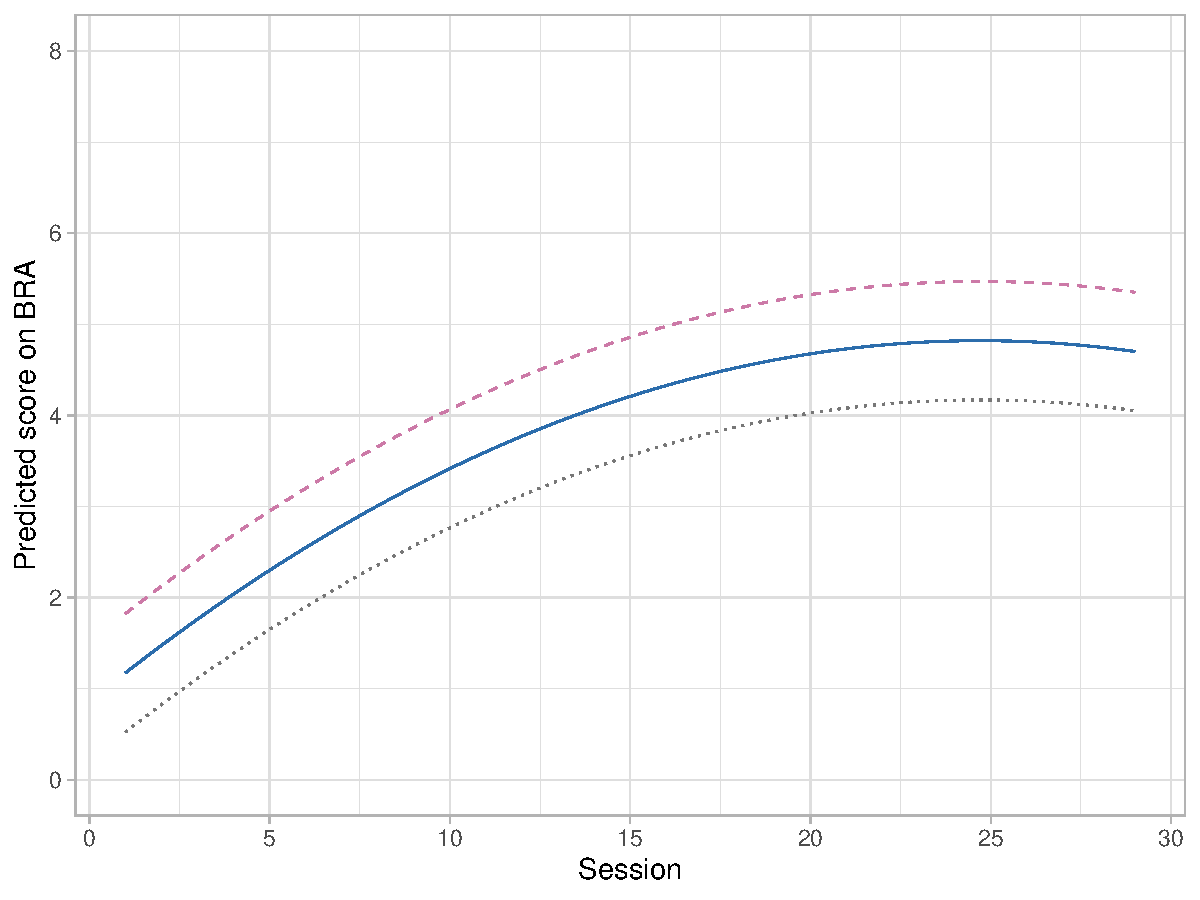
\includegraphics[width=0.8\linewidth]{thesis_files/figure-latex/fitted-model-g-1} 

}

\caption[Fitted curve for Model G showing the average predicted change in bivariate reasoning across class session for students with below average (grey, dotted), average (blue, solid), and above average (reddish purple, dashed) change in their reasoning about distribution]{Fitted curve for Model G showing the average predicted change in bivariate reasoning across class session for students with below average (grey, dotted), average (blue, solid), and above average (reddish purple, dashed) change in their reasoning about distribution.}\label{fig:fitted-model-g}
\end{figure}

\hypertarget{examining-and-interpreting-a-final-conditional-model}{%
\section{Examining and Interpreting a Final Conditional Model}\label{examining-and-interpreting-a-final-conditional-model}}

Now that each of the main effect models for the important predictors has been examined and interpreted, a final model can be postulated. One variable that might need to be controlled for is teacher (coded \(-1\) and \(+1\)). Initially, a model was fit using all three predictors (teacher, instructional sequence, and students' change in reasoning about distribution) at each level along with both two-way, and three-way interactions. The \emph{F}-statistic to test the composite hypotheses for the three-way fixed effects was non-significant---\(F(3,~134)=0.76,~p=0.52\)---so those terms were dropped from the model. The two-way interaction fixed effects were tested in the same fashion and subsequently dropped from the model---\(F(9,~189)=0.61,~p=0.79\). A series of more parsimonious models were then examined and compared. The resulting ``final model'' is presented in \ref{tab:model-h}.

\begingroup\fontsize{10}{12}\selectfont
\begin{table}[ht]
\caption{\label{tab:model-h}Final conditional model to examine students' change in reasoning about bivariate data}
\centering
\fontsize{10}{12}\selectfont
\begin{tabular}{p{3in}P{1in}P{1.5in}}
\toprule
\thead{Effects} & \thead{Parameter} & \thead{Model H}\\
\midrule
\multicolumn{3}{l}{\textbf{Fixed effects}} \\[1ex]
Intercept & $\gamma_{00}$ & 0.84$^{***}$\\[1ex]
DRA$-\bar{\mathrm{DRA}}$ & $\gamma_{01}$ & 0.07\\[1ex]
Teacher & $\gamma_{02}$ & $-0.21^{\sim}$\\[1ex]
Session & $\gamma_{10}$ & 0.32$^{***}$\\[1ex]
Teacher $\times$ Session & $\gamma_{11}$ & 0.02$^{*}$\\[1ex]
Session$^2$ & $\gamma_{20}$ &$-0.01^{***}$ \\[1ex]
DRA$-\bar{\mathrm{DRA}}$ $\times$ Session$^2$ & $\gamma_{21}$ & 0.0002$^{\sim}$\\[1ex]
\addlinespace[0.3em]
\multicolumn{3}{l}{\textbf{Variance components}} \\[1ex]
Level-1: Within student & $\sigma^2_{\epsilon}$ & $1.08^{***}$\\[1ex]
Level-2: Between student & \\[1ex]
\hspace{1em}Var(Linear term) & $\sigma^2_{1}$ &  $0.01^{**}$\\[1ex]
\hspace{1em}Var(Quadratic term) & $\sigma^2_{2}$ &  $0.00001^{\sim}$\\[1ex]
\hspace{1em}Cov(Linear, Quadratic) & $\sigma_{12}$ & $-0.0004^{\sim}$\\[1ex]
\addlinespace[0.3em]
\multicolumn{3}{l}{\textbf{Goodness-of-fit}} \\[1ex]
Deviance & & 1451.7\\[1ex]
AIC & & 1471.7\\[1ex]
BIC & & 1511.9 \\[1ex]
\bottomrule
\multicolumn{3}{l}{$^{\sim}p<0.10~^{*}p<0.05,~^{**}p<0.01,~^{***}p<0.001$}\\
\end{tabular}
\end{table}
\endgroup

\hypertarget{model-h-the-final-conditional-model}{%
\subsection{Model H: The Final Conditional Model}\label{model-h-the-final-conditional-model}}

Model H includes both sequence and change in reasoning about univariate distribution as predictors, as well as controlling for the effects of different teachers. The fixed-effects suggest that a student who exhibits average change in his/her reasoning about univariate distribution has an initial BRA score of 0.84 (\(p<0.001\)) when controlling for teacher. The average initial BRA score also seems to be different for students who have different teachers. The BRA scores for students who had one teacher rather than another differ on average by 0.21 (\(p<0.10\)) when controlling for differences in centered DRS scores. There seems to be no association between the linear rates of change in BRA score and centered DRS score when controlling for teacher. However, there does seem to be a slight average difference in the linear rates of change of BRA scores between students who have different teachers. This average difference is small, but significantly larger than zero at 0.02 (\(p<0.10\)).

The fixed-effects for the quadratic rate of change suggest that students on average have an estimated average quadratic rate of change of \(-0.01\) (\(p<0.001\)). There is also a small positive association (0.0002, \(p<0.10\)) between students' quadratic rates of change and their centered DRS scores. This indicates that students with above average change in their DRS scores tend to have larger quadratic rate of change terms. The trajectories of growth by teacher moderated by centered DRS score are shown in \ref{fig:fitted-model-h}. The variance components remain largely unchanged from previous models.

\begin{figure}[H]

{\centering 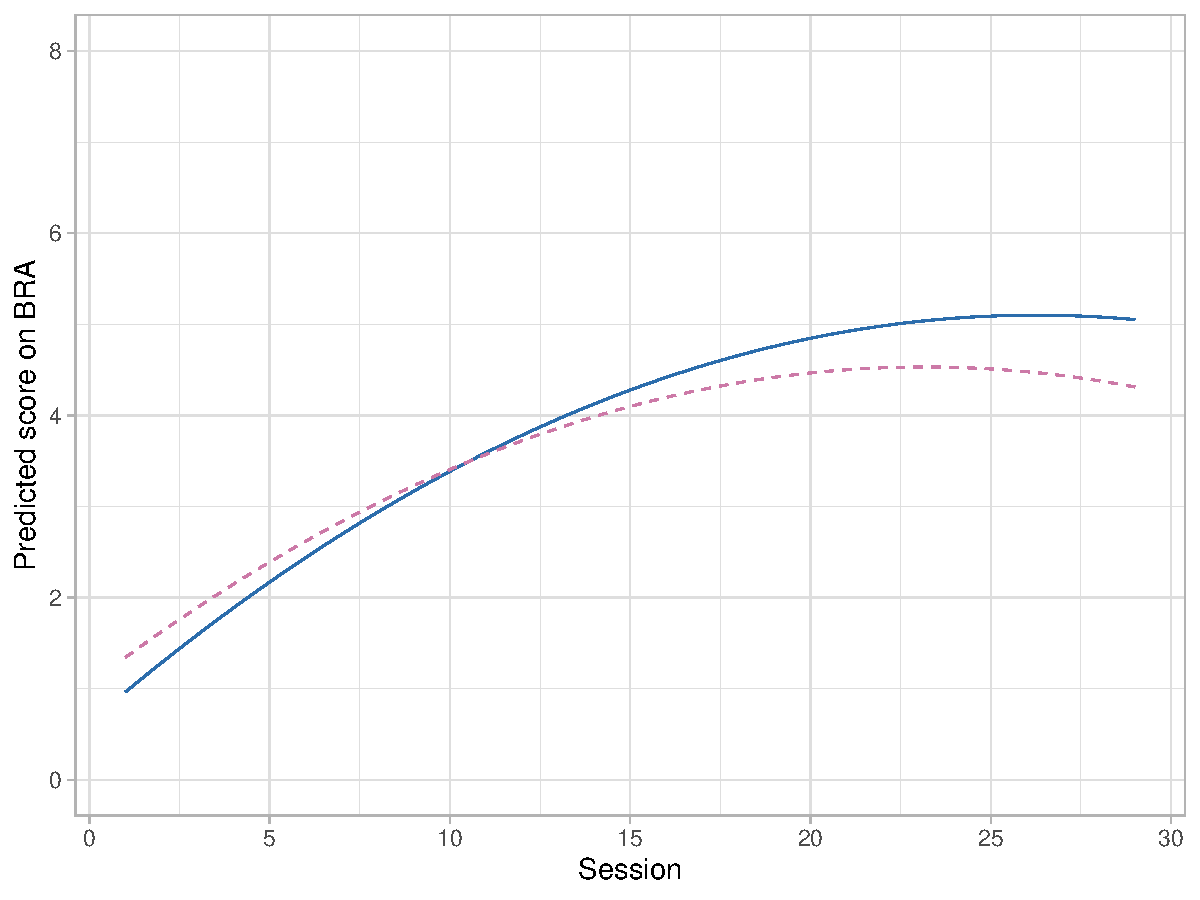
\includegraphics[width=0.8\linewidth]{thesis_files/figure-latex/fitted-model-h-1} 

}

\caption[Fitted curve for Model H showing the average predicted change in bivariate reasoning across class session for students with  average change in their reasoning about distribution for the two teachers, Teacher A (blue, solid) and Teacher B (reddish purple, dashed)]{Fitted curve for Model H showing the average predicted change in bivariate reasoning across class session for students with  average change in their reasoning about distribution for the two teachers, Teacher A (blue, solid) and Teacher B (reddish purple, dashed).}\label{fig:fitted-model-h}
\end{figure}

This chapter presented the results from the study. There were several models that were examined in describing both students' change in development of reasoning about bivariate data, as well as in attempting to account for those changes by introducing relevant predictors into the model. The next chapter will lay out and summarize the findings from this study, and also describe what they might mean for the field of statistics education.

\hypertarget{discussion}{%
\chapter{Discussion}\label{discussion}}

This chapter summarizes the main contributions of the study's research findings to the general field of statistics education. It will focus on how the study has addressed each of the research questions in turn, and offer both further analysis and reflection. It will then articulate some limitations of the research and outline some implications for future research.

The study described in this dissertation examined the change in students' development in reasoning about bivariate data. To measure change in students' reasoning, the quantitative bivariate data scale from the \emph{Assessment Resource Tools for Improving Statistical Thinking} (ARTIST) was administered to 113 students four times during a one-semester introductory statistics course. These students were also assessed on their distributional reasoning four times during the course of the semester using ten items from the \emph{Comprehensive Assessment of Outcomes in a First Statistics course} (CAOS) in order to determine if changes in reasoning about the foundational concepts of distribution were associated with changes in the development of reasoning about bivariate data.

In order to determine if the sequencing of bivariate data within a course is associated with changes in the pattern of change in students' reasoning about bivariate data, the two instructors of the course were used as blocks to randomly assign each section of the course to one of two different course sequences. Both of these course sequences began with the topic of sampling and experimental design followed by exploratory data analysis on univariate distributions. After univariate distribution, one of the course sequences taught the topic of bivariate data and then concluded with topics consisting of sampling distributions, probability, and inference. The other course sequence followed the topic of univariate distribution with those of sampling distributions, probability, and inference with the topic of bivariate data being the last topic taught in the course.

Students were also measured on several other factors to examine if any of them might explain the pattern of change in students' reasoning about bivariate data, and also to serve as controls when comparing the four sections of the course. Ten released items from the 2003 \emph{Trends in International Mathematics and Science Study} (TIMSS) grade-8 mathematics test were administered to students to measure their prior algebra knowledge, and the entire 40-item CAOS was administered to measure prior statistical knowledge. Fifteen survey items that were adapted from the 2005 questionnaire used to examine students' mathematical backgrounds on the grade-12 \emph{National Assessment of Educational Progress} (NAEP) were also given to students to help examine their mathematics background. Lastly, students' ACT composite scores were obtained after the completion of the semester and used as a measure of students' general knowledge These measures were examined as potential covariates to help explain the pattern in students' development of reasoning about bivariate data.

To examine the change in students' covariational reasoning, this study utilized linear mixed-effects models (LMMs) in attempt to not only examine the temporal pattern of development, but to determine how that development was influenced by instructional sequence and development in univariate reasoning. In particular, this study sought to answer three research questions:

\begin{enumerate}
\def\labelenumi{\arabic{enumi}.}
\tightlist
\item
  What is the nature, or pattern of change in students' development in reasoning about bivariate data?
\item
  Is the sequencing of bivariate data within a course associated with changes in the pattern of development in students' reasoning about bivariate data?
\item
  Are changes in students' reasoning about the foundational concepts of distribution associated with changes in the pattern of development in students' reasoning about bivariate data?
\end{enumerate}

\hypertarget{research-question-1}{%
\section{Research Question 1}\label{research-question-1}}

Students in this study seemed to exhibit growth in their reasoning about bivariate data. The LMM that was adopted to examine this growth suggested that students exhibit both linear and quadratic growth in their development about reasoning about bivariate data and that this growth varies among individual students. A quadratic model indicates that students' reasoning about bivariate data does not increase in a constant linear fashion, but instead increases differentially over time. The significant negative quadratic term suggests that although students initially show great strides in their reasoning about bivariate data, they eventually plane off in this development and over time might actually even regress. This pattern of development, consistent with several different learning theories (e.g., overlapping waves theory; \protect\hyperlink{ref-siegler:2000}{Siegler, 2000}), might suggest that a saturation point in bivariate reasoning is reached by students and then decay or interference impedes any more growth in reasoning during the course (e.g., \protect\hyperlink{ref-wixted:2004}{Wixted, 2004}).

The model also suggested that on average students without any instruction start with very little reasoning about bivariate data and that this is true for nearly all students. This could be because almost all of the students used in this study had never had a previous statistics course. However, the low initial status leaves much to be desired, especially since covariation is recognized and promoted by NCTM in the mathematics curriculum at nearly every age level. This might be explained by the fact that many of these students hadn't had a mathematics course in several years prior to taking statistics, but it might also be because reasoning is not a major focus of most mathematics courses.

While the fixed-effects and random-effects terms for intercept, linear rate of change and quadratic rate of change were all statistically significant, the practical significance might not be as important. For instance, the variance terms associated with the quadratic rate of change was statistically significant (\(p<0.05\)) indicating that students vary in their quadratic rates of change. However, the actual variance term was 0.0000121. This small variance component indicates that students' quadratic rates of change are very similar. Also, comparatively, the within-student variance component still accounts for the majority of the variation in BRA scores.

One interesting finding is that most of the change in development in reasoning about bivariate data seemed to occur between the first two measurement occasions. This was before bivariate data was formally taught in either instructional sequence. This might indicate that students' development in reasoning about bivariate data is more an artifact of their development to reason about statistics in general than it is a result of any formal instruction on the topic of bivariate data. However, the brevity of the unit within this particular introductory statistics class (four instructional sessions) might also inhibit an increase in development of reasoning due to instruction about this topic. It also might mean that students' reasoning about bivariate data is closely tied to their reasoning about univariate distribution as suggested by the statistics education literature (e.g., \protect\hyperlink{ref-cobb:2003a}{Cobb, McClain, et al., 2003}; \protect\hyperlink{ref-gravemeijer:2000}{Gravemeijer, 2000}).

This study has in some sense, broken new ground in the field of statistics education. The literature has, to date, not examined the development of students' reasoning about bivariate data. Perhaps this study could be used as a model for how student development of reasoning could be studied in an introductory statistics course.

\hypertarget{research-question-2}{%
\section{Research Question 2}\label{research-question-2}}

The sequencing of bivariate data within a course seemed not to be associated with changes in students' development of reasoning about bivariate data either as a solitary covariate, or in conjunction with other covariates. There seemed to be no differences in either the linear or quadratic rates of change in covariational reasoning between the two instructional sequences. The fact that sequencing was not important in explaining patterns of development might not be surprising if, as stated before, reasoning about bivariate data is just a byproduct of reasoning about statistics in general.

Finding no differences in students' reasoning between the two sequences might suggest that the topic could be placed wherever the instructor or textbook authors decided. As a word of caution, however, while the development in reasoning about bivariate data might not change as a result of the placement of this topic, student development of reasoning about other topics might be impacted. One of these topics could be inference. While this wasn't tested formally in this study, some anecdotal evidence, such as students' complaints and discussion, suggests that students in the class where bivariate data was taught earlier seemed to be struggling with inference more than students in the other classes. It might also be that bivariate data is a topic that is more ``digestible'' than inference at the end of a semester.

Course sequencing has also received little attention in the statistics education literature. While Chance and Rossman (\protect\hyperlink{ref-chance:2001}{2001}) have speculated about the placement of a unit on bivariate data, there has been no research on optimal placement of this, or for that matter any other topic within an introductory statistics course. The literature on textbook usage has, however, suggested that the content and sequencing of textbooks could influence how effectively students will learn that content (e.g., \protect\hyperlink{ref-valverde:2002}{Valverde et al., 2002}). While this study found no effect on students' growth based on where the unit on bivariate data was placed, research questions involving course content and sequence need more attention.

\hypertarget{research-question-3}{%
\section{Research Question 3}\label{research-question-3}}

This study initially seemed to suggest that change in reasoning about univariate distribution was not associated with students' development of reasoning about bivariate data. However, once the effects of teacher were controlled for, changes in reasoning about distribution were important in explaining the quadratic rate of change in covariational reasoning. The model suggested students who exhibited higher than average change in their reasoning about univariate distribution tended to also have higher quadratic terms in their patterns of development (the level-1 equations). This indicates that those students will exhibit less loss of reasoning about bivariate data throughout the duration of an introductory statistics course.

While the association between change in reasoning about univariate distribution and quadratic change in reasoning about bivariate data was statistically significant, the practical significance is rather dubious. The coefficient was very small, indicating very little difference in the quadratic rate of change for those students who had a higher than average and those students who had a less than average change in their reasoning about univariate distribution.

There also seemed to be a teacher difference both in initial status (which has nothing to do with the teacher) and in linear rate of change. While linear change in covariational reasoning might be due to the teacher, it could also be that those students who started lower are just catching up so to speak.

The findings from this research question are also somewhat novel. The research literature on students' reasoning about bivariate data has been generally speculative. While Cobb, McClain, and Gravemeijer (\protect\hyperlink{ref-cobb:2003a}{2003}) and @Gravemeijer (\protect\hyperlink{ref-gravemeijer:2000}{2000}) have all suggested that students need to be able to reason about univariate distribution before they can reason about bivariate data, there have been no studies that have examined this hypothesis. Perhaps the pattern of change in reasoning exhibited by students in this study lends some credence to these speculations. Since most of the growth in reasoning about bivariate data occurred during the instruction of univariate distribution, perhaps these two types of reasoning are inextricably connected.

\hypertarget{limitations}{%
\section{Limitations}\label{limitations}}

There are many limitations to this research that need to be mentioned. One limitation concerns both the sample size (\(n=113\)) and the number of measurement occasions (\(t=4\)). One hundred thirteen students (level-1 units) is a very small sample size in the realm of multi-level modeling. Small sample sizes may result in less efficiency and power of multilevel tests. With less than adequate power there is an unacceptable risk of not detecting cross-level interactions (e.g., between students and measurement occasions). However, both adequate number of individual observations and adequate number of students are needed, since power for level-1 estimates depends on number of measurement occasions, and power for level-2 estimates depends on number of students.

Generalization may also be limited due to the type of introductory statistics students that were used in the study. These students were typically female social science majors. This does not adequately describe most introductory statistics students. However, while these students may have not been typical in terms of demographics, they might be typical in terms of initial levels of reasoning and background for students enrolled in a non-calculus based first semester statistics course.

Another limitation in this study is the instruments that were utilized. The reliability of scores for the reasoning instruments, while tolerable, could be higher. Also, while most students did not reach the maximum score on the assessments, a few students did get perfect scores. This may have limited the variability in scores and thereby impacted the LMM coefficients. The instruments to measure covariates, such as algebra knowledge, also produced unreliable scores. This might have hindered the identification of differences between groups of students.

Another limitation was the number of students who returned the ACT consent form. While the use of social exchange (\protect\hyperlink{ref-dillman:2000}{Dillman, 2000}) was thought to increase the response rate, there were still a number of students who opted not to consent to release their ACT score. One possible solution might have been to have students self-report that data, but studies have suggested that students' self-reports of these test scores are not reliable at all (\protect\hyperlink{ref-cassady:2001}{Cassady, 2001}).

Missing data might also have impacted the findings for the third research question as well. Since only 98 students had measurements on the fourth occasion, the sample was reduced due to the fact that not every student had a difference score (level-2 predictor) for this model. While this missingness was thought to be random (due only to student absence) there is no way for the applied researcher to be sure of this unless he/she had the very data they do not have. Thus, while these observations were identified as missing at random and therefore the model parameters should be un-biased, there is no way to be sure.

Finally, while every effort was made to ensure consistency between the two teachers, much like snowflakes, there are no two instructors who teach the same way. This unavoidable inconsistency might have affected growth in such a way as to ``cover up'' differences due to one of the tested level-2 predictors. In larger studies this can be accounted for by using a three-level model where not only are measurements nested within students, but students are also nested within teachers. Thus, the variation can be further partitioned and accounted for. However, the small number of teachers (\(k=2\)) did not allow this type of model to converge in this study.

\hypertarget{implications-for-teaching}{%
\section{Implications for Teaching}\label{implications-for-teaching}}

While there were many limitations connected with this study, the results suggest some practical implications for teachers of introductory statistics. One implication is that instruction in topics related to univariate distribution (e.g., center, spread) may have great impact on students' reasoning on many other topics within the introductory statistics curriculum. This is shown in the pattern of students' development where the most growth occurred during the instruction of univariate distribution. This importance of univariate distribution is made even more salient by the significance of this factor on the development of students' reasoning about bivariate data. The idea of spending ample time developing students' reasoning about univariate distribution is also consistent with recommendations in the statistics education literature (e.g., \protect\hyperlink{ref-asa:2005}{American Statistical Association, 2005a}; \protect\hyperlink{ref-iase:2005}{International Association for Statistical Education, 2005})

Secondly, the sequencing of topics within an introductory course needs to be given more thought. While this study did not show a change in students' reasoning about bivariate data based on where the unit was sequenced, it might have an effect on students' reasoning about other topics, such as inference. Since so many topics are interconnected in the introductory statistics curriculum, it would make a great deal of sense that the course sequence might affect student reasoning.

\hypertarget{future-research}{%
\section{Future Research}\label{future-research}}

There is a great deal of need for research on growth within an introductory statistics course. With the new ASA endorsed GAISE guidelines, the introductory statistics course will change in future years. It is an important educational goal to determine which factors in an introductory statistics course influence students' growth. Is it the teacher? The curriculum? Student interactions? Or is it the individual student?

To this end, one still prominent research question is not only how the placement of a unit on bivariate data influences students' development in covariational reasoning, but how that placement affects the development of reasoning about other topics within an introductory statistics course such as inference. Questions about the best sequencing of curriculum within an introductory statistics course are important not only in how they impact students' learning and reasoning about statistics in general, but in how those sequences impact students' reasoning of sub-topics within a course.

Another interesting line of research is how foundational topics in an introductory statistics course influence students' development of reasoning about other topics. While this study examined how changes in students' reasoning about distribution influenced their reasoning about bivariate data, perhaps a different study might look at how students' reasoning about variation might influence reasoning about bivariate data or other statistical reasoning.

Researchers interested in change in students' reasoning about statistical concepts might use this as a springboard. This study has employed a methodology that allows researchers to examine students' development of reasoning in an introductory statistics course in the ecology of an actual classroom. It has also made an attempt at using randomization in classroom research. While far from the ideal of educational research, this study may provide statistics education researchers with insight and direction in terms of design and methodology. The results of this study may also suggest some future research in the study of students' development of statistical reasoning. For instance, it seems that much of the variation in students' change in reasoning is within-student variation. This implies the need to add a time-varying (level-1) predictor. It would be worthwhile for researchers to consider what predictors at level-1 might account for this variation. Likewise, on average students did not differ on many of the level-2 covariates. It would be wise for statistics educators to identify predictors that may account for the level-2 variation. While these might be difficult to identify \emph{a priori}, the research literature may provide some guidance. For instance, many studies have suggested that prior mathematics and statistics experience are not predictive of students' ability to reason (e.g., \protect\hyperlink{ref-konold:1999}{Konold, 1999}).

Future researchers might want to use a non-linear model to depict student development. Non-linear models have been used to model change in student development (e.g., \protect\hyperlink{ref-mcardle:1987}{McArdle \& Epstein, 1987}). This might be more in line with learning theory (e.g., \protect\hyperlink{ref-min:2000}{Min et al., 2000}; \protect\hyperlink{ref-murre:2006}{Murre \& Chessa, 2006}; \protect\hyperlink{ref-wozniak:1990}{Wozniak, 1990}). For instance, the use of the logistic curve to model population growth (\protect\hyperlink{ref-verhulst:1845}{Verhulst, 1845}) was adapted by Pearl (\protect\hyperlink{ref-pearl:1925}{1925}) to model cognitive growth. Another example of non-linear growth to describe learning is the hyperbolic curve outlined by Thurston (\protect\hyperlink{ref-thurston:1919}{1919}).

In summary, the study of change of students' reasoning requires multiple measurements over time. The current methodologies used to study change (e.g., structural equation modeling, multi-level modeling) require the same assessment to be used at each time point. This is generally not pedagogically acceptable to most college teachers given the time constraints that accompany collegiate courses. Even more complicated is the fact that to model a complex growth pattern requires more measurement occasions, especially during times that students are exhibiting the most change, such as near the beginning of the semester (\protect\hyperlink{ref-willet:1998}{Willet et al., 1998}; \protect\hyperlink{ref-willett:1989}{Willett, 1989}). This frequent testing could have a negative impact on student attitudes and cause early fatigue in study subjects. As the call for growth studies by policy makers and interested parties increases, careful attention should be given to the methodologies and the practical problems faced by educators in their implementation.

\hypertarget{references}{%
\chapter*{References}\label{references}}
\addcontentsline{toc}{chapter}{References}

\noindent

\setlength{\parindent}{-0.20in}
\setlength{\leftskip}{0.20in}
\setlength{\parskip}{8pt}

\hypertarget{refs}{}
\begin{CSLReferences}{1}{0}
\leavevmode\vadjust pre{\hypertarget{ref-act:1997}{}}%
ACT. (1997). \emph{{ACT} assessment technical manual}. ACT, Inc.

\leavevmode\vadjust pre{\hypertarget{ref-adi:1978}{}}%
Adi, H., Karplus, R., Lawson, A., \& Pulos, S. (1978). Intellectual development beyond elementary school VI: Correlational reasoning: AESOP. \emph{School Science and Mathematics}, \emph{78}(8), 675--683.

\leavevmode\vadjust pre{\hypertarget{ref-akaike:1974}{}}%
Akaike, H. (1974). A new look at the statistical model identification. \emph{IEEE Transactions on Automatic Control}, \emph{19}(6), 716--723. \url{https://doi.org/10.1109/TAC.1974.1100705}

\leavevmode\vadjust pre{\hypertarget{ref-alloy:1979}{}}%
Alloy, L. B., \& Abramson, L. Y. (1979). Judgment of contingency in depressed and nondepressed students: Sadder but wiser? \emph{Journal of Experimental Psychology. General}, \emph{108}(4), 441--485.

\leavevmode\vadjust pre{\hypertarget{ref-alloy:1984}{}}%
Alloy, L. B., \& Tabachnik, N. (1984). Assessment of covariation by humans and animals: The joint influence of prior expectations and current situational information. \emph{Psychological Review}, \emph{91}(1), 112--149. \url{https://doi.org/10.1037/0033-295X.91.1.112}

\leavevmode\vadjust pre{\hypertarget{ref-alvermann:1987}{}}%
Alvermann, D. E. (1987). The role of textbooks in teachers' interactive decision making. \emph{Reading Research and Instruction}, \emph{26}(2), 115--127. \url{https://doi.org/10.1080/19388078709557902}

\leavevmode\vadjust pre{\hypertarget{ref-alvermann:1989}{}}%
Alvermann, D. E. (1989). Teacher‐student mediation of content area texts. \emph{Theory Into Practice}, \emph{28}(2), 142--147. \url{https://doi.org/10.1080/00405848909543393}

\leavevmode\vadjust pre{\hypertarget{ref-asa:2005}{}}%
American Statistical Association. (2005a). \emph{GAISE college report}. \url{http://www.amstat.org/education/gaise/GAISECollege.htm}

\leavevmode\vadjust pre{\hypertarget{ref-asa:2005a}{}}%
American Statistical Association. (2005b). \emph{{GAISE} endorsement}. \url{http://www.amstat.org/education/gaise/ASAEndorse.htm.}

\leavevmode\vadjust pre{\hypertarget{ref-anderson:1991}{}}%
Anderson, J. R., \& Schooler, L. J. (1991). Reflections of the environment in memory. \emph{Psychological Science}, \emph{2}(6), 396--408. \url{https://doi.org/10.1111/j.1467-9280.1991.tb00174.x}

\leavevmode\vadjust pre{\hypertarget{ref-anderson:2005}{}}%
Anderson, R. B., Doherty, M. E., Berg, N. D., \& Friedrich, J. C. (2005). Sample size and the detection of correlation--a signal detection account: Comment on {K}areev (2000) and {J}uslin and {O}lsson (2005). \emph{Psychological Review}, \emph{112}(1), 268--279. \url{https://doi.org/10.1037/0033-295X.112.1.268}

\leavevmode\vadjust pre{\hypertarget{ref-arkes:1983}{}}%
Arkes, H. R., \& Harkness, A. R. (1983). Estimates of contingency between two dichotomous variables. \emph{Journal of Experimental Psychology: General}, \emph{112}(1), 117--135. \url{https://doi.org/10.1037/0096-3445.112.1.117}

\leavevmode\vadjust pre{\hypertarget{ref-atkinson:1965}{}}%
Atkinson, R. C., Bower, G. H., \& Crothers, E. J. (1965). \emph{An introduction to mathematical learning theory}. John Wiley.

\leavevmode\vadjust pre{\hypertarget{ref-australian-education-council:1994}{}}%
Australian Education Council. (1994). \emph{Mathematics---a curriculum profile for {A}ustralian schools}. Curriculum Corporation.

\leavevmode\vadjust pre{\hypertarget{ref-barr:1988}{}}%
Barr, R. (1988). Conditions influencing content taught in nine fourth-grade mathematics classrooms. \emph{The Elementary School Journal}, \emph{88}(4), 387--411. \url{https://doi.org/10.1086/461546}

\leavevmode\vadjust pre{\hypertarget{ref-batanero:1997}{}}%
Batanero, C., Estepa, A., \& Godino, J. D. (1997). Evolution of students' understanding of statistical association in a computer based teaching environment. In J. B. Garfield \& G. Burrill (Eds.), \emph{Research on the role of technology in teaching and learning statistics: Proceedings of the 1996 {IASE Round Table Conference}} (pp. 191--205). International Statistical Institute.

\leavevmode\vadjust pre{\hypertarget{ref-batanero:1996}{}}%
Batanero, C., Estepa, A., Godino, J. D., \& Green, D. R. (1996). Intuitive strategies and preconceptions about association in contingency tables. \emph{Journal for Research in Mathematics Education}, \emph{27}(2), 151--169. \url{https://doi.org/10.2307/749598}

\leavevmode\vadjust pre{\hypertarget{ref-batanero:1998}{}}%
Batanero, C., Godino, J. D., \& Estepa, A. (1998). First international research forum on statistical reasoning, thinking, and literacy. In J. Garfield \& D. Ben-Zvi (Eds.), \emph{Building the meaning of statistical association through data analysis activities} (pp. 37--53).

\leavevmode\vadjust pre{\hypertarget{ref-bates:2005a}{}}%
Bates, D. (2005, July 13). \emph{\[R\] testing for significance in random-effect factors using lmer}. Message posted to {R}-help. \url{http://tolstoy.newcastle.edu.au/R/help/05/07/8420.html}

\leavevmode\vadjust pre{\hypertarget{ref-bates:2005}{}}%
Bates, D., \& Sarkar, D. (2005). \emph{lme4: Linear mixed-effects models using {S4} classes}. {R package version 0.98-1}.

\leavevmode\vadjust pre{\hypertarget{ref-beach:1966}{}}%
Beach, L. R., \& Scopp, T. S. (1966). Inferences about correlations. \emph{Psychonomic Science}, \emph{6}(6), 253--254. \url{https://doi.org/10.3758/BF03328053}

\leavevmode\vadjust pre{\hypertarget{ref-beaton:1996}{}}%
Beaton, A. E., Mullis, I. V. S., Martin, M. O., Gonzalez, E. J., Kelly, D. L., \& Smith, T. A. (1996). \emph{{Mathematics achievement in middle school years: IEA's Third International Mathematics and Science Study (TIMSS)}}. Center for the Study of Testing, Evaluation,; Educational Policy, Boston College.

\leavevmode\vadjust pre{\hypertarget{ref-ben-zvi:2004}{}}%
Ben-Zvi, D., \& Garfield, J. (2004). Statistical literacy, reasoning, and thinking: Goals, definitions, and challenges. In D. Ben-Zvi \& J. Garfield (Eds.), \emph{The challenge of developing statistical literacy, reasoning, and thinking} (pp. 3--15). Kluwer Academic Publishers.

\leavevmode\vadjust pre{\hypertarget{ref-bettman:1986}{}}%
Bettman, J. R., John, D. R., \& Scott, C. A. (1986). Covariation assessment by consumers. \emph{Journal of Consumer Research}, \emph{13}(3), 316--326. \url{https://doi.org/10.1086/209071}

\leavevmode\vadjust pre{\hypertarget{ref-beyth-marom:1982}{}}%
Beyth-Marom, R. (1982). Perception of correlation reexamined. \emph{Memory \& Cognition}, \emph{10}, 511--519.

\leavevmode\vadjust pre{\hypertarget{ref-blau:1964}{}}%
Blau, P. M. (1964). \emph{Exchange and power in social life}. Wiley.

\leavevmode\vadjust pre{\hypertarget{ref-bobko:1979}{}}%
Bobko, P., \& Karren, R. (1979). The perception of {P}earson product moment correlations from bivariate scatterplots. \emph{Personnel Psychology}, \emph{32}(2), 313--325. \url{https://doi.org/10.1111/j.1744-6570.1979.tb02137.x}

\leavevmode\vadjust pre{\hypertarget{ref-borovcnik:1984}{}}%
Borovcnik, M. G. (1984). The role of descriptive statistics. In A. Bell \& and J. K. B. Low (Eds.), \emph{Theory, research and practice in mathematical education} (pp. 285--292). Shell Centre for Mathematical Education.

\leavevmode\vadjust pre{\hypertarget{ref-boyle:2001}{}}%
Boyle, \&. W., Michael H. (2001). Multilevel modelling of hierarchical data in developmental studies. \emph{Journal of Child Psychology and Psychiatry}, \emph{42}(1), 141--162. \url{https://doi.org/10.1111/1469-7610.00706}

\leavevmode\vadjust pre{\hypertarget{ref-bush:1986}{}}%
Bush, W. S. (1986). Preservice teachers' sources of decisions in teaching secondary mathematics. \emph{Journal for Research in Mathematics Education}, \emph{17}(1), 21--30.

\leavevmode\vadjust pre{\hypertarget{ref-campbell:1966}{}}%
Campbell, D. T., \& Stanley, J. C. (1966). \emph{Experimental and quasi-experimental designs}. Rand McNally Publishing Co.

\leavevmode\vadjust pre{\hypertarget{ref-carlson:1998}{}}%
Carlson, M. (1998). A cross-sectional investigation of the development of the function concept. In E. Dubinsky, A. H. Schoenfeld, \& J. J. Kaput (Eds.), \emph{Research in collegiate mathematics education III, issues in mathematics education} (Vol. 7, pp. 115--162).

\leavevmode\vadjust pre{\hypertarget{ref-carlson:2002a}{}}%
Carlson, M. (2002). Physical enactment: A powerful representational tool for understanding the nature of covarying relationships. In F. Hitt (Ed.), \emph{Representations and mathematics visualization} (pp. 63--77). CINVESTAV.

\leavevmode\vadjust pre{\hypertarget{ref-carlson:2002}{}}%
Carlson, M., Jacobs, S., Coe, E., Larsen, S., \& Hsu, E. (2002). Applying covariational reasoning while modeling dynamic events: A framework and a study. \emph{Journal for Research in Mathematics Education}, \emph{33}(5), 352--378.

\leavevmode\vadjust pre{\hypertarget{ref-carlson:2001}{}}%
Carlson, M., Larsen, S., \& Jacobs, S. (2001). An investigation of covariational reasoning and its role in learning the concepts of limit and accumulation. In R. Speiser, C. Maher, \& C. Walter (Eds.), \emph{Proceedings of the 23rd annual meeting of the {North American Chapter of the International Group for the Psychology of Mathematics Education}} (Vol. 1, pp. 145--153). PME-NA.

\leavevmode\vadjust pre{\hypertarget{ref-cassady:2001}{}}%
Cassady, J. C. (2001). Self-reported {GPA} and {SAT}: A methodological note. \emph{Practical Assessment, Research \& Evaluation}, \emph{7}(12).

\leavevmode\vadjust pre{\hypertarget{ref-chance:2001}{}}%
Chance, B. L., \& Rossman, A. J. (2001). Sequencing topics in introductory statistics: A debate on what to teach when. \emph{The American Statistician}, \emph{55}(2), 140--144.

\leavevmode\vadjust pre{\hypertarget{ref-chapman:1967}{}}%
Chapman, L. J. (1967). Illusory correlation in observational report. \emph{Journal of Verbal Learning and Verbal Behavior}, \emph{6}, 151--155.

\leavevmode\vadjust pre{\hypertarget{ref-chapman:1967a}{}}%
Chapman, L. J., \& Chapman, J. P. (1967). Genesis of popular but erroneous psychodiagnostic observations. \emph{Journal of Abnormal Psychology}, \emph{72}(3), 193--204. \url{https://doi.org/10.1037/h0024670}

\leavevmode\vadjust pre{\hypertarget{ref-chapman:1969}{}}%
Chapman, L. J., \& Chapman, J. P. (1969). Illusory correlations as an obstacle to the use of valid psychodiagnostic tests. \emph{Journal of Abnormal Psychology}, \emph{74}, 271--280.

\leavevmode\vadjust pre{\hypertarget{ref-cheng:1997}{}}%
Cheng, P. W. (1997). From covariation to causation: A causal power theory. \emph{Psychological Review}, \emph{104}(2), 367--405.

\leavevmode\vadjust pre{\hypertarget{ref-cheng:1990}{}}%
Cheng, P. W., \& Novick, L. R. (1990). A probabilistic contrast model of causal induction. \emph{Journal of Personality and Social Psychology}, \emph{58}(4), 545--567.

\leavevmode\vadjust pre{\hypertarget{ref-cheng:1992}{}}%
Cheng, P. W., \& Novick, L. R. (1992). Covariation in natural causal induction. \emph{Psychological Review}, \emph{99}(2), 365--382.

\leavevmode\vadjust pre{\hypertarget{ref-cleveland:1982}{}}%
Cleveland, W. S., Diaconis, P., \& McGill, R. (1982). Variables on scatterplots look more highly correlated when the scales are increased. \emph{Science}, \emph{216}, 1138--1141.

\leavevmode\vadjust pre{\hypertarget{ref-cobb:2000}{}}%
Cobb, G. (2000). Teaching statistics: More data, less lecturing. In T. L. Moore (Ed.), \emph{Resources for undergraduate instructors: Teaching statistics} (pp. 3--8). Mathematical Association of America.

\leavevmode\vadjust pre{\hypertarget{ref-cobb:2005}{}}%
Cobb, G. (2005). Forword. In \emph{Innovations in teaching statistics} (pp. vii--viii). Mathematical Association of America.

\leavevmode\vadjust pre{\hypertarget{ref-cobb:1998}{}}%
Cobb, P. (1998). Theorizing about mathematical conversations and learning from practice. \emph{For the Learning of Mathematics}, \emph{18}(1), 46--48.

\leavevmode\vadjust pre{\hypertarget{ref-cobb:2003}{}}%
Cobb, P., Confrey, J., diSessa, A., Lehrer, R., \& Schauble, L. (2003). Design experiments in educational research. \emph{Educational Researcher}, \emph{32}(1), 9--13. \url{https://doi.org/10.3102/0013189X032001009}

\leavevmode\vadjust pre{\hypertarget{ref-cobb:2003a}{}}%
Cobb, P., McClain, K., \& Gravemeijer, K. P. E. (2003). Learning about statistical covariation. \emph{Cognition and Instruction}, \emph{21}(1), 1--78.

\leavevmode\vadjust pre{\hypertarget{ref-college-board:2003}{}}%
College Board. (2003). \emph{Advanced placement statistics course guide}. {College Board}.

\leavevmode\vadjust pre{\hypertarget{ref-collins:2001}{}}%
Collins, L. M., Schafer, J. L., \& Kam, C.-M. (2001). A comparison of inclusive and restrictive strategies in modern missing data procedures. \emph{Psychological Methods}, \emph{6}(4), 330--351. \url{https://doi.org/10.1037/1082-989X.6.4.330}

\leavevmode\vadjust pre{\hypertarget{ref-crocker:1981}{}}%
Crocker, J. (1981). Judgment of covariation by social perceivers. \emph{Psychological Bulletin}, \emph{90}(2), 272--292.

\leavevmode\vadjust pre{\hypertarget{ref-crocker:1982}{}}%
Crocker, J. (1982). Biased questions in judgement of studies. \emph{Personality and Social Psychological Bulletin}, \emph{8}(2), 214--220. \url{https://doi.org/10.1177/0146167282082005}

\leavevmode\vadjust pre{\hypertarget{ref-cronbach:1951}{}}%
Cronbach, L. J. (1951). Coefficient alpha and the internal structure of tests. \emph{Psychometrika}, \emph{16}, 297--333. \url{https://doi.org/10.1007/BF02310555}

\leavevmode\vadjust pre{\hypertarget{ref-curtis:1986}{}}%
Curtis, J. B. (1986). \emph{Teaching college biology students the simple linear regression model using an interactive microcomputer graphics software program} {[}PhD thesis{]}. University of Wisconsin-Madison.

\leavevmode\vadjust pre{\hypertarget{ref-davis:1964}{}}%
Davis, F. B. (1964). Measurement of change. In F. B. Davis (Ed.), \emph{Educational measurements and their interpretation} (pp. 234--252). Wadsworth.

\leavevmode\vadjust pre{\hypertarget{ref-delmas:2006}{}}%
delMas, R., Garfield, J., Ooms, A., \& Chance, B. (2006). \emph{Assessing students' conceptual understanding after a first course in statistics}. Paper presented at the annual meeting of the {A}merican {E}ducational {R}esearch {A}ssociation, {S}an {F}rancisco, {CA}.

\leavevmode\vadjust pre{\hypertarget{ref-department-for-education-and-employment:1999}{}}%
Department for Education and Employment. (1999). \emph{Mathematics: The national curriculum for {E}ngland}. Author; Qualifications; Curriculum Authority.

\leavevmode\vadjust pre{\hypertarget{ref-diggle:1988}{}}%
Diggle, P. J. (1988). An approach to the analysis of repeated measures. \emph{Biometrics}, \emph{45}, 1255--1258.

\leavevmode\vadjust pre{\hypertarget{ref-dillman:2000}{}}%
Dillman, D. A. (2000). \emph{Mail and internet surveys: The {T}ailored design method}. John Wiley \& Sons, Inc.

\leavevmode\vadjust pre{\hypertarget{ref-ebbinghaus:1885}{}}%
Ebbinghaus, H. (1885; English 1913). \emph{Memory a contribution to experimental psychology} (H. A. Ruger \& C. E. Bussenius, Trans.). Teachers College, Columbia University.

\leavevmode\vadjust pre{\hypertarget{ref-einhorn:1986}{}}%
Einhorn, H. J., \& Hogarth, R. M. (1986). Judging probable cause. \emph{Psychological Bulletin}, \emph{99}(1), 3--19.

\leavevmode\vadjust pre{\hypertarget{ref-erlick:1966}{}}%
Erlick, D. E. (1966). Human estimates of statistical relatedness. \emph{Psychonomic Science}, \emph{5}, 365--366.

\leavevmode\vadjust pre{\hypertarget{ref-erlick:1967}{}}%
Erlick, D. E., \& Mills, R. G. (1967). Perceptual quantification of conditional dependency. \emph{Journal of Experimental Psychology}, \emph{73}(1), 9--14. \url{https://doi.org/10.1037/h0024138}

\leavevmode\vadjust pre{\hypertarget{ref-ertmer:1993}{}}%
Ertmer, P. A., \& Newby, T. J. (1993). Behaviorism, cognitivism, constructivism: Comparing critical features from an instructional design perspective. \emph{Performance Improvement Quarterly}, \emph{6}(4), 50--72. \url{https://doi.org/10.1111/j.1937-8327.1993.tb00605.x}

\leavevmode\vadjust pre{\hypertarget{ref-estepa:2001}{}}%
Estepa, A., \& Sánchez Cobo, F. T. (2001). Empirical research on the understanding of association and implications for the training of researchers. In C. Batanero (Ed.), \emph{Training researchers in the use of statistics} (pp. 37--51). IASE.

\leavevmode\vadjust pre{\hypertarget{ref-estes:1950}{}}%
Estes, W. K. (1950). Toward a statistical theory of learning. \emph{Psychological Review}, \emph{57}(2), 94--107. \url{https://doi.org/10.1037/h0058559}

\leavevmode\vadjust pre{\hypertarget{ref-fan:2000}{}}%
Fan, L., \& Kaeley, G. S. (2000). The influence of textbook on teaching strategies: An empirical study. \emph{Mid-Western Educational Researcher}, \emph{13}(4), 2--9.

\leavevmode\vadjust pre{\hypertarget{ref-fiedler:1991}{}}%
Fiedler, K. (1991). The tricky nature of skewed frequency tables: An information loss account of distinctiveness-based illusory correlations. \emph{Journal of Personality and Social Psychology}, \emph{60}(1), 24--36. \url{https://doi.org/10.1037/0022-3514.60.1.24}

\leavevmode\vadjust pre{\hypertarget{ref-freeman:1989}{}}%
Freeman, D. J., \& Porter, A. C. (1989). Do textbooks dictate the content of mathematics instruction in elementary schools? \emph{American Educational Research Journal}, \emph{26}(3), 403--421. \url{https://doi.org/10.3102/00028312026003403}

\leavevmode\vadjust pre{\hypertarget{ref-garfield:1995}{}}%
Garfield, J. (1995). How students learn statistics. \emph{International Statistical Review}, \emph{63}(1), 25--34.

\leavevmode\vadjust pre{\hypertarget{ref-garfield:2002}{}}%
Garfield, J. (2002). The challenge of developing statistical reasoning. \emph{Journal of Statistics Education}, \emph{10}(3). \url{https://doi.org/10.1080/10691898.2002.11910676}

\leavevmode\vadjust pre{\hypertarget{ref-garfield:2003}{}}%
Garfield, J. (2003). Assessing statistical reasoning. \emph{Statistics Education Research Journal}, \emph{2}(1), 22--38.

\leavevmode\vadjust pre{\hypertarget{ref-garfield:1988}{}}%
Garfield, J., \& Ahlgren, A. (1988). Difficulties in learning basic concepts in probability and statistics: Implications for research. \emph{Journal for Research in Mathematics Education}, \emph{19}(1), 44--63.

\leavevmode\vadjust pre{\hypertarget{ref-garfield:2000}{}}%
Garfield, J., \& Chance, B. (2000). Assessment in statistics education: Issues and challenges. \emph{Mathematical Thinking and Learning}, \emph{2}(1--2), 99--125.

\leavevmode\vadjust pre{\hypertarget{ref-garfield:nd}{}}%
Garfield, J., delMas, R., \& Chance, B. (n.d.). \emph{{Assessment Resource Tools for Improving Statistical Thinking}}.

\leavevmode\vadjust pre{\hypertarget{ref-gelman:2002}{}}%
Gelman, A., \& Nolan, D. (2002). \emph{Teaching statistics: A bag of tricks}. Oxford University Press.

\leavevmode\vadjust pre{\hypertarget{ref-gravemeijer:2000}{}}%
Gravemeijer, K. P. E. (2000). \emph{A rationale for an instructional sequence for analyzing one- and two-dimensional data sets}. Paper presented at the annual meeting of the {American Educational Research Association}, {M}ontreal, {C}anada.

\leavevmode\vadjust pre{\hypertarget{ref-gray:1968}{}}%
Gray, C. (1968). Predicting with intuitive correlations. \emph{Psychonomic Science}, \emph{11}(2), 41--42.

\leavevmode\vadjust pre{\hypertarget{ref-gulliksen:1987}{}}%
Gulliksen, H. (1987). \emph{Theory of mental tests}. Routledge. \url{https://doi.org/10.4324/9780203052150}

\leavevmode\vadjust pre{\hypertarget{ref-hamilton:1976}{}}%
Hamilton, D. L., \& Gifford, R. (1976). Illusory correlation in interpersonal perception: A cognitive basis of stereotypic judgments. \emph{Journal of Personality and Social Psychology}, \emph{39}, 832--845.

\leavevmode\vadjust pre{\hypertarget{ref-hamilton:1980}{}}%
Hamilton, D. L., \& Rose, T. L. (1980). Illusory correlation and the maintenance of stereotypic beliefs. \emph{Journal of Experimental Social Psychology}, \emph{12}, 392--407.

\leavevmode\vadjust pre{\hypertarget{ref-haslam:1994}{}}%
Haslam, S. A., \& McGarty, C. (1994). Problems with the measurement of illusory correlation. \emph{European Journal of Social Psychology}, \emph{24}, 611--621.

\leavevmode\vadjust pre{\hypertarget{ref-heider:1958}{}}%
Heider, F. (1958). \emph{The psychology of interpersonal relationships}. Wiley.

\leavevmode\vadjust pre{\hypertarget{ref-hilgard:1975}{}}%
Hilgard, E. R., \& Bower, G. H. (1975). \emph{Theories of learning} (4th ed.). Prentice-Hall.

\leavevmode\vadjust pre{\hypertarget{ref-inhelder:1958}{}}%
Inhelder, B., \& Piaget, J. (1958). \emph{The growth of logical thinking from childhood to adolescence}. Routledge \& Kegan Paul.

\leavevmode\vadjust pre{\hypertarget{ref-iase:2005}{}}%
International Association for Statistical Education. (2005). \emph{{SRTL}-4 report}. \url{http://www.stat.auckland.ac.nz/~iase/.}

\leavevmode\vadjust pre{\hypertarget{ref-iaeea:2005}{}}%
International Association for the Evaluation of Educational Achievement. (2005). \emph{{TIMSS} 2003 mathematics items: Released set eighth grade}. International Study Centre, Lynch School of Education, Boston College.

\leavevmode\vadjust pre{\hypertarget{ref-jennings:1982}{}}%
Jennings, D., Amabile, T., \& Ross, L. (1982). Informal covariation assessment: Data-based versus theory-based judgments. In D. Kahneman, P. Slovic, \& A. Tversky (Eds.), \emph{Judgment under uncertainty: Heuristics and biases} (pp. 211--230). Cambridge University Press.

\leavevmode\vadjust pre{\hypertarget{ref-kao:1993}{}}%
Kao, S.-F., \& Wasserman, E. A. (1993). Assessment of an information integration account of contingency judgment with examination of subjective cell importance and method of information presentation. \emph{Journal of Experimental Psychology: Learning, Memory, and Cognition}, \emph{19}(6), 1363--1386. \url{https://doi.org/10.1037/0278-7393.19.6.1363}

\leavevmode\vadjust pre{\hypertarget{ref-kaput:1992}{}}%
Kaput, J. J. (1992). Patterns in students' formalization of quantitative patterns. In G. Harel \& E. Dubinsky (Eds.), \emph{The concept of function: Aspects of epistemology and pedagogy} (Vol. 25, pp. 290--318). Mathematical Association of America.

\leavevmode\vadjust pre{\hypertarget{ref-kelley:1967}{}}%
Kelley, H. (1967). Attribution theory in social psychology. In D. Levine (Ed.), \emph{Nebraska symposium on motivation} (Vol. 15). University of Nebraska Press.

\leavevmode\vadjust pre{\hypertarget{ref-kon:1993}{}}%
Kon, J. H. (1993). \emph{The thud at the classroom door: Teachers' curriculum decision making in response to a new textbook} {[}PhD thesis{]}. Stanford University.

\leavevmode\vadjust pre{\hypertarget{ref-konarski:2005}{}}%
Konarski, R. (2005). Judgments of correlation from scatterplots with contaminated distributions. \emph{Polish Psychological Bulletin}, \emph{36}(1), 51--62.

\leavevmode\vadjust pre{\hypertarget{ref-konold:1999}{}}%
Konold, C. (1999). Issues in assessing conceptual understanding in probability and statistics. \emph{Journal of Statistics Education}, \emph{3}(1).

\leavevmode\vadjust pre{\hypertarget{ref-konold:2002}{}}%
Konold, C. (2002). Teaching concepts rather than conventions. \emph{New England Journal of Mathematics}, \emph{34}(2), 69--81.

\leavevmode\vadjust pre{\hypertarget{ref-konold:2002a}{}}%
Konold, C., \& Higgins, T. L. (2002). Highlights of related research. In S. J. Russell, D. Schifter, \& V. Bastable (Eds.), \emph{Developing mathematical ideas: Working with data} (pp. 165--201). Dale Seymour Publications.

\leavevmode\vadjust pre{\hypertarget{ref-krammer:1985}{}}%
Krammer, H. P. M. (1985). The textbook as classroom context variable. \emph{Teaching and Teacher Education}, \emph{1}(4), 273--278. \url{https://doi.org/10.1016/0742-051X(85)90015-0}

\leavevmode\vadjust pre{\hypertarget{ref-kuhn:1989}{}}%
Kuhn, D. (1989). Children and adults as intuitive scientists. \emph{Psychological Review}, \emph{96}(4), 674--689. \url{https://doi.org/10.1037/0033-295X.96.4.674}

\leavevmode\vadjust pre{\hypertarget{ref-kuhn:1988}{}}%
Kuhn, D., Amsel, E., \& O'Loughlin, M. (1988). \emph{The development of scientific thinking skills}. Academic Press.

\leavevmode\vadjust pre{\hypertarget{ref-kuhn:1977}{}}%
Kuhn, D., \& Brannock, J. (1977). Development of the isolation of variables scheme in experimental and {``natural experiment''} contexts. \emph{Developmental Psychology}, \emph{13}(1), 9--14.

\leavevmode\vadjust pre{\hypertarget{ref-kuhn:1995}{}}%
Kuhn, D., Garcia-Mila, M., Zohar, A., \& Andersen, C. (1995). Strategies of knowledge acquisition. \emph{Monographs of the Society for Research in Child Development}, \emph{60}(4), 1--128.

\leavevmode\vadjust pre{\hypertarget{ref-kuhn:1977a}{}}%
Kuhn, D., \& Ho, V. (1977). The development of schemes for recognizing additive and alternative effects in a {``natural experiment''} context. \emph{Developmental Psychology}, \emph{13}(5), 515--516. \url{https://doi.org/10.1037/0012-1649.13.5.515}

\leavevmode\vadjust pre{\hypertarget{ref-kuhs:1979}{}}%
Kuhs, T. M., \& Freeman, D. J. (1979). \emph{The potential influence of textbooks on teachers' selection of content for elementary school mathematics}. {Paper presented at the annual meeting of the American Educational Research Association. San Francisco}.

\leavevmode\vadjust pre{\hypertarget{ref-lane:1985}{}}%
Lane, D. M., Anderson, C. A., \& Kellam, K. L. (1985). Judging the relatedness of variables: The psychophysics of covariation detection. \emph{Journal of Experimental Psychology: Human Perception and Performance}, \emph{11}(5), 640--649. \url{https://doi.org/10.1037/0096-1523.11.5.640}

\leavevmode\vadjust pre{\hypertarget{ref-lawson:1982}{}}%
Lawson, A. E. (1982). The relative responsiveness of concrete operational seventh grade and college students to science instruction. \emph{Journal of Research in Science Teaching}, \emph{19}(1), 63--77. \url{https://doi.org/10.1002/tea.3660190109}

\leavevmode\vadjust pre{\hypertarget{ref-lawson:1979}{}}%
Lawson, A. E., Adi, H., \& Karplus, R. (1979). Development of correlational reasoning in secondary schools: Do biology courses make a difference? \emph{American Biology Teacher}, \emph{41}(7), 420--425, 430.

\leavevmode\vadjust pre{\hypertarget{ref-lawson:2003}{}}%
Lawson, T. J., Schwiers, M., Doellman, M., Grady, G., \& Kelnhofer, R. (2003). Enhancing students' ability to use statistical reasoning with everyday problems. \emph{Teaching of Psychology}, \emph{30}(2), 107--110.

\leavevmode\vadjust pre{\hypertarget{ref-levin:1993}{}}%
Levin, I. P., Wasserman, E. A., \& Kao, S.-F. (1993). Multiple methods for examining biased information use in contingency judgments. \emph{Organizational Behavior and Human Decision Processes}, \emph{55}, 228--250.

\leavevmode\vadjust pre{\hypertarget{ref-lewandowsky:1989}{}}%
Lewandowsky, S., \& Spence, I. (1989). Discriminating strata in scatterplots. \emph{Journal of the American Statistical Association}, \emph{84}(407), 682--688. \url{https://doi.org/10.2307/2289649}

\leavevmode\vadjust pre{\hypertarget{ref-lipe:1990}{}}%
Lipe, M. G. (1990). A lens-model analysis of covariation research. \emph{Journal of Behavioral Decision Making}, \emph{3}, 47--59.

\leavevmode\vadjust pre{\hypertarget{ref-little:1995}{}}%
Little, R. J. A. (1995). Modeling the dropout mechanism in repeated-measures studies. \emph{Journal of the American Statistical Association}, \emph{90}(431), 1112--1121. \url{https://doi.org/10.2307/2291350}

\leavevmode\vadjust pre{\hypertarget{ref-lovell:1961}{}}%
Lovell, K. (1961). A follow-up study of inhelder and piaget's {``the growth of logical thinking.''} \emph{The British Journal of Psychology}, \emph{52}(2), 143--153.

\leavevmode\vadjust pre{\hypertarget{ref-lutzer:2000}{}}%
Lutzer, D. J., Maxwell, J. W., \& Rodi, S. B. (2000). \emph{Statistical abstract of undergraduate programs in the mathematical sciences in the united states: Fall 2000 {CBMS} survey}. American Mathematical Society.

\leavevmode\vadjust pre{\hypertarget{ref-mcardle:1987}{}}%
McArdle, J. J., \& Epstein, D. (1987). Latent growth curves within developmental structural equation models. \emph{Child Development}, \emph{58}, 110--133.

\leavevmode\vadjust pre{\hypertarget{ref-mccutcheon:1981}{}}%
McCutcheon, G. (1981). How do elementary school teachers plan? The nature of planning and influences on it. \emph{Elementary School Journal}, \emph{81}(1), 4--23. \url{https://doi.org/10.1086/461201}

\leavevmode\vadjust pre{\hypertarget{ref-mccutcheon:1982}{}}%
McCutcheon, G. (1982). \emph{Textbook use in a central {O}hio elementary school}. {Paper presented at the annual meeting of the American Educational Research Association. (ERIC Document Reproduction Service No. ED 216 968)}.

\leavevmode\vadjust pre{\hypertarget{ref-mcgahan:1997}{}}%
McGahan, J. R., Flynn, S., Williamson, J. D., \& McDougal, B. (1997). \emph{An alternate-forms approach to reliability assessment for intuitive covariation judgments}. Paper presented at the annual meeting of the {Southwestern Psychological Association}, {Fort Worth, TX}.

\leavevmode\vadjust pre{\hypertarget{ref-mcgahan:2000}{}}%
McGahan, J. R., McDougal, B., Williamson, J. D., \& Pryor, P. L. (2000). The equivalence of contingency structure for intuitive covariation judgments about height, weight, and body fat. \emph{Journal of Psychology}, \emph{134}, 325--335.

\leavevmode\vadjust pre{\hypertarget{ref-mcgarty:1993}{}}%
McGarty, C., Haslam, A., Turner, J. C., \& Oakes, P. J. (1993). Illusory correlation as accentuation of actual intercategory difference: Evidence for the effect with minimal stimulus information. \emph{European Journal of Social Psychology}, \emph{23}, 391--410.

\leavevmode\vadjust pre{\hypertarget{ref-mckenzie:inpress}{}}%
McKenzie, C. R. M., \& Mikkelsen, L. A. (in press). A bayesian view of covariation assessment. \emph{Cognitive Psychology}.

\leavevmode\vadjust pre{\hypertarget{ref-mckenzie:1986}{}}%
McKenzie, D. L., \& Padilla, M. J. (1986). The construction and validation of the {Test of Graphing in Science (TOGS)}. \emph{Journal of Research in Science Teaching}, \emph{23}(7), 571--579. \url{https://doi.org/10.1002/tea.3660230702}

\leavevmode\vadjust pre{\hypertarget{ref-mensink:1988}{}}%
Mensink, G.-J., \& Raaijmakers, J. G. (1988). A model for interference and forgetting. \emph{Psychological Review}, \emph{95}(4), 434--455. \url{https://doi.org/10.1037/0033-295X.95.4.434}

\leavevmode\vadjust pre{\hypertarget{ref-meyer:1997}{}}%
Meyer, J., Taieb, M., \& Flascher, I. (1997). Correlation estimates as perceptual judgments. \emph{Journal of Experimental Psychology: Applied}, \emph{3}(1), 3--20.

\leavevmode\vadjust pre{\hypertarget{ref-min:2000}{}}%
Min, R., Vos, H., Kommers, P., \& van Dijkum, C. (2000). A concept model for learning: An attempt to define a proper relations scheme between instruction and learning and to establish the dynamics of learning in relation to motivation, intelligence and study- ability ({``studeerbaarheid''}). \emph{Journal of Interactive Learning Research}, \emph{11}(3/4), 485--506.

\leavevmode\vadjust pre{\hypertarget{ref-ministry-of-education:1992}{}}%
Ministry of Education. (1992). \emph{Mathematics in the {N}ew {Z}ealand curriculum}. Ministry of Education.

\leavevmode\vadjust pre{\hypertarget{ref-monk:1992}{}}%
Monk, S. (1992). Students' understanding of a function given by a physical model. In G. Harel \& E. Dubinsky (Eds.), \emph{The concept of function: Aspects of epistemology and pedagogy} (Vol. 25, pp. 175--193). Mathematical Association of America.

\leavevmode\vadjust pre{\hypertarget{ref-monk:1994}{}}%
Monk, S., \& Nemirovsky, R. (1994). The case of {D}an: Student construction of a functional situation through visual attributes. In E. Dubinsky, J. Kaput, \& A. Schoenfeld (Eds.), \emph{Research in collegiate mathematics education} (Vol. 1, pp. 139--168). American Mathematics Society.

\leavevmode\vadjust pre{\hypertarget{ref-moritz:2004}{}}%
Moritz, J. B. (2004). Reasoning about covariation. In D. Ben-Zvi \& J. Garfield (Eds.), \emph{The challenge of developing statistical literacy, reasoning, and thinking} (pp. 227--256). Kluwer Academic Publishers.

\leavevmode\vadjust pre{\hypertarget{ref-morris:1997}{}}%
Morris, E. (1997). \emph{An investigation of students' conceptions and procedural skills in the statistical topic correlation}. {CITE Report. No. 230. Centre for Information Technology in Education. Institute of Educational Technology. The Open University}.

\leavevmode\vadjust pre{\hypertarget{ref-mullen:1990}{}}%
Mullen, B., \& Johnson, C. (1990). Distinctiveness-based illusory correlations and stereotyping: A meta-analytic integration. \emph{British Journal of Social Psychology}, \emph{29}, 11--28.

\leavevmode\vadjust pre{\hypertarget{ref-murphy:1994}{}}%
Murphy, R. (1994). The effects of task characteristics on covariation assessment: The impact of accountability and judgment frame. \emph{Organizational Behavior and Human Decision Processes}, \emph{60}(1), 139--155. \url{https://doi.org/10.1006/obhd.1994.1078}

\leavevmode\vadjust pre{\hypertarget{ref-murre:2006}{}}%
Murre, J. M. J., \& Chessa, A. G. (2006). \emph{A model of learning and forgetting {II}: The learning curve}.

\leavevmode\vadjust pre{\hypertarget{ref-nadel:2000}{}}%
Nadel, L., Samsonovich, A., Ryan, L., \& Moscovitch, M. (2000). Multiple trace theory of human memory: Computational, neuroimaging, and neuropsychological results. \emph{Hippocampus}, \emph{10}(4), 352--368.

\leavevmode\vadjust pre{\hypertarget{ref-nagb:2003}{}}%
National Assessment Governing Board. (2003). \emph{Background information framework for the {National Assessment of Educational Progress}}. U.S. Department of Education.

\leavevmode\vadjust pre{\hypertarget{ref-nctm:2000}{}}%
National Council of Teachers of Mathematics. (2000). \emph{Principles and standards for school mathematics}. {National Council of Teachers of Mathematics}.

\leavevmode\vadjust pre{\hypertarget{ref-neidorf:2004}{}}%
Neidorf, T. S., \& Garden, R. (2004). Developing the {TIMSS} 2003 mathematics and science assessment and scoring guides. In M. O. Martin, I. V. S. Mullis, \& S. J. Chrostowski (Eds.), \emph{{TIMSS} 2003 technical report} (pp. 23--65). TIMSS \& PIRLS International Study Center, Boston College.

\leavevmode\vadjust pre{\hypertarget{ref-neimark:1975}{}}%
Neimark, E. (1975). Longitudinal development of formal operations thought. \emph{Genetic Psychology Monographs}, \emph{91}, 175--225.

\leavevmode\vadjust pre{\hypertarget{ref-nemirovsky:1996}{}}%
Nemirovsky, R. (1996). A functional approach to algebra: Two issues that emerge. In N. Dedrarg, C. Kieran, \& L. Lee (Eds.), \emph{Approaches to algebra: Perspectives for research and teaching} (pp. 295--313). Kluwer Academic Publishers.

\leavevmode\vadjust pre{\hypertarget{ref-nisbett:1980}{}}%
Nisbett, R., \& Ross, L. (1980). \emph{Human inference: Strategies and shortcomings of social judgment}. Prentice-Hall.

\leavevmode\vadjust pre{\hypertarget{ref-padilla:1986}{}}%
Padilla, M. J., McKenzie, D. L., \& Shaw, E. L. (1986). An examination of the line graphing ability of students in grades seven through twelve. \emph{School Science and Mathematics}, \emph{86}(1), 20--26. \url{https://doi.org/10.1111/J.1949-8594.1986.TB11581.X}

\leavevmode\vadjust pre{\hypertarget{ref-pearl:1925}{}}%
Pearl, R. (1925). \emph{The biology of population growth}. Knopf.

\leavevmode\vadjust pre{\hypertarget{ref-peterson:1980}{}}%
Peterson, C. (1980). Recognition of noncontingency. \emph{Journal of Personality and Social Psychology}, \emph{38}(5), 727--734. \url{https://doi.org/10.1037/0022-3514.38.5.727}

\leavevmode\vadjust pre{\hypertarget{ref-pinheiro:2000}{}}%
Pinheiro, J., \& Bates, D. (2000). \emph{Mixed-effects models in {S} and {S-PLUS}}. Springer Verlag.

\leavevmode\vadjust pre{\hypertarget{ref-pinheiro:2005}{}}%
Pinheiro, J., Bates, D., DebRoy, S., \& Sarkar, D. (2005). \emph{Nlme: Linear and nonlinear mixed-effects models}. {R package version 3.1-66}.

\leavevmode\vadjust pre{\hypertarget{ref-pryor:2000}{}}%
Pryor, P. L., McGahan, J. R., Hutto, C. W., \& Willliamson, J. D. (2000). A preliminary study of the effect of imaginary sexual stimulation on the perceived covariation between freedom and responsibility. \emph{The Journal of Psychology}, \emph{134}(6), 645--658. \url{https://doi.org/10.1080/00223980009598243}

\leavevmode\vadjust pre{\hypertarget{ref-r-dev:2005}{}}%
R Development Core Team. (2005). \emph{R: A language and environment for statistical computing}. {R Foundation for Statistical Computing, Vienna, Austria}. \url{http://www.R-project.org}

\leavevmode\vadjust pre{\hypertarget{ref-raaijmakers:1981}{}}%
Raaijmakers, J. G., \& Shiffrin, R. M. (1981). Search of associative memory. \emph{Psychological Review}, \emph{88}(2), 93--134. \url{https://doi.org/10.1037/0033-295X.88.2.93}

\leavevmode\vadjust pre{\hypertarget{ref-raudenbush:2002}{}}%
Raudenbush, S. W., \& Bryk, A. S. (2002). \emph{Hierarchical linear models: Applications and data analysis methods}. Sage Publications, Inc.

\leavevmode\vadjust pre{\hypertarget{ref-robinson:1985}{}}%
Robinson, F. G., Ross, J. A., \& White, F. (1985). \emph{Curriculum development for effective instruction}. Ontario Institute for Studies in Education Press.

\leavevmode\vadjust pre{\hypertarget{ref-ross:1993}{}}%
Ross, J. A., \& Cousins, J. B. (1993). Patterns of student growth in reasoning about correlational problems. \emph{Journal of Educational Psychology}, \emph{85}(1), 49--65. \url{https://doi.org/10.1037/0022-0663.85.1.49}

\leavevmode\vadjust pre{\hypertarget{ref-ross:1981}{}}%
Ross, J. A., \& Maynes, F. J. (1981). \emph{Geographic thinking skills}. Ontario Institute for Studies in Education Press.

\leavevmode\vadjust pre{\hypertarget{ref-saldanha:1998}{}}%
Saldanha, L. A., \& Thompson, P. W. (1998). Re-thinking co-variation from a quantitative perspective: Simultaneous continuous variation. In S. B. Berensen, K. R. Dawkins, M. Blanton, W. N. Coulombe, J. Kolb, K. Norwood, \& L. Stiff (Eds.), \emph{{Proceedings of the 20th annual meeting of the North American Chapter of the International Group for the Psychology of Mathematics Education}} (Vol. 1, pp. 298--303). ERIC Clearinghouse for Science, Mathematics,; Environmental Education.

\leavevmode\vadjust pre{\hypertarget{ref-sanchez:1999}{}}%
Sánchez, F. T. (1999). \emph{Significado de la correlación y regression para los estudiantes universitarios ({M}eanings of correlation and regression for undergraduates)} {[}PhD thesis{]}. University of Granada.

\leavevmode\vadjust pre{\hypertarget{ref-schmidt:2001}{}}%
Schmidt, W. H., McKnight, C. C., Houang, R. T., Wang, H. C., Wiley, D. E., Cogan, L. S., \& Wolfe, R. G. (2001). \emph{Why schools matter: Using {TIMSS} to investigate curriculum and learning}. Jossey-Bass Publishers.

\leavevmode\vadjust pre{\hypertarget{ref-schustack:1981}{}}%
Schustack, M. W., \& Sternberg, R. J. (1981). Evaluation of evidence in causal inference. \emph{Journal of Experimental Psychology: General}, \emph{110}(1), 101--120. \url{https://doi.org/10.1037/0096-3445.110.1.101}

\leavevmode\vadjust pre{\hypertarget{ref-schwarz:1978}{}}%
Schwarz, G. (1978). Estimating the dimension of a model. \emph{The Annals of Statistics}, \emph{6}(2), 461--464.

\leavevmode\vadjust pre{\hypertarget{ref-seggie:1972}{}}%
Seggie, J. L., \& Endersby, H. (1972). The empirical implications of {P}iaget's concept of correlation. \emph{Australian Journal of Psychology}, \emph{24}(1), 3--8. \url{https://doi.org/10.1080/00049537208255778}

\leavevmode\vadjust pre{\hypertarget{ref-shaklee:1988}{}}%
Shaklee, H., \& Elek, S. (1988). Cause and covariate: Development of two related concepts. \emph{Cognitive Development}, \emph{3}(1), 1--13. \url{https://doi.org/10.1016/0885-2014(88)90027-5}

\leavevmode\vadjust pre{\hypertarget{ref-shaklee:1989}{}}%
Shaklee, H., \& Goldston, D. (1989). Development in causal reasoning: Information sampling and judgment rule. \emph{Cognitive Development}, \emph{4}(3), 269--281. \url{https://doi.org/10.1016/0885-2014(89)90009-9}

\leavevmode\vadjust pre{\hypertarget{ref-shaklee:1981}{}}%
Shaklee, H., \& Mims, M. (1981). Development of rule use in judgments of covariation between events. \emph{Child Development}, \emph{52}(1), 317--325. \url{https://doi.org/10.2307/1129245}

\leavevmode\vadjust pre{\hypertarget{ref-shaklee:1983}{}}%
Shaklee, H., \& Paszek, D. (1983). \emph{Eliciting systematic rule use in covariation judgment (the early years)}. (Report No. NIE-6-80-0091). Washington DC: National Institute of Education.

\leavevmode\vadjust pre{\hypertarget{ref-shaklee:1980}{}}%
Shaklee, H., \& Tucker, D. (1980). A rule analysis of judgments of covariation between events. \emph{Memory \& Cognition}, \emph{8}(5), 459--467. \url{https://doi.org/10.3758/BF03211142}

\leavevmode\vadjust pre{\hypertarget{ref-shultz:1975}{}}%
Shultz, T. R., \& Mendelson, R. (1975). The use of covariation as a principle of causal analysis. \emph{Child Development}, \emph{46}(2), 394--399. \url{https://doi.org/10.2307/1128133}

\leavevmode\vadjust pre{\hypertarget{ref-siegler:2000}{}}%
Siegler, R. S. (2000). The rebirth of children's learning. \emph{Child Development}, \emph{71}(1), 26--35.

\leavevmode\vadjust pre{\hypertarget{ref-simon:1995}{}}%
Simon, M. A. (1995). Reconstructing mathematics pedagogy from a constructivist perspective. \emph{Journal for Research in Mathematics Education}, \emph{26}, 114--145.

\leavevmode\vadjust pre{\hypertarget{ref-singer:2003}{}}%
Singer, J. D., \& Willett, J. B. (2003). \emph{Applied longitudinal data analysis}. Oxford University Press.

\leavevmode\vadjust pre{\hypertarget{ref-smedslund:1963}{}}%
Smedslund, J. (1963). The concept of correlation in adults. \emph{Scandinavian Journal of Psychology}, \emph{4}, 165--173.

\leavevmode\vadjust pre{\hypertarget{ref-smith:1981}{}}%
Smith, E. E. (1981). \emph{Categories and concepts}. Harvard University Press.

\leavevmode\vadjust pre{\hypertarget{ref-snyder:1981}{}}%
Snyder, M. (1981). Seek and ye shall find: Testing hypotheses about other people. In E. T. Higgins, D. C. Herman, \& M. P. Zanna (Eds.), \emph{Social cognition: The {Ontario Symposium on Personality and Social Psychology}}. Erlbaum.

\leavevmode\vadjust pre{\hypertarget{ref-snyder:1978}{}}%
Snyder, M., \& Swann, W. B. (1978). Hypothesis\mbox{-}testing processes in social interaction. \emph{Journal of Personality and Social Psychology}, \emph{36}(11), 1202--1212.

\leavevmode\vadjust pre{\hypertarget{ref-sosniak:1993}{}}%
Sosniak, L. A., \& Stodolsky, S. S. (1993). Teachers and textbooks: Materials use in four fourth-grade classrooms. \emph{The Elementary School Journal}, \emph{93}(3), 249--275. \url{https://doi.org/10.1086/461725}

\leavevmode\vadjust pre{\hypertarget{ref-spellman:1996}{}}%
Spellman, B. A. (1996). Acting as intuitive scientists: Contingency judgments are made while controlling for alternative potential causes. \emph{Psychological Science}, \emph{7}(6), 337--342. \url{https://doi.org/10.1111/j.1467-9280.1996.tb00385.x}

\leavevmode\vadjust pre{\hypertarget{ref-steffe:1991}{}}%
Steffe, L. P. (1991). The constructivist teaching experiment: Illustrations and implications. In E. von Glassersfeld (Ed.), \emph{Radical constructivism in mathematics education} (pp. 177--194). Kluwer Academic Press.

\leavevmode\vadjust pre{\hypertarget{ref-steffe:2000}{}}%
Steffe, L. P., \& Thompson, P. W. (2000). Teaching experiment methodology: Underlying principles and essential elements. In R. Lesh \& A. E. Kelly (Eds.), \emph{Research design in mathematics and science education} (pp. 267--307). Erlbaum.

\leavevmode\vadjust pre{\hypertarget{ref-stockburger:1982}{}}%
Stockburger, D. W. (1982). Evaluation of three simulation exercises in an introductory statistics course. \emph{Contemporary Educational Psychology}, \emph{7}(4), 365--370.

\leavevmode\vadjust pre{\hypertarget{ref-stodolsky:1989}{}}%
Stodolsky, S. S. (1989). Is teaching really by the book? In P. W. Jackson \& S. Haroutunian-Gordon (Eds.), \emph{{From Socrates to software: The teacher as text and the text as teacher: Eighty-eighth yearbook of the National Society for the Study of Education, Part I}} (pp. 159--184). University of Chicago Press.

\leavevmode\vadjust pre{\hypertarget{ref-strahan:1978}{}}%
Strahan, R. F., \& Hansen, C. J. (1978). Underestimating correlation from scatterplots. \emph{Applied Psychological Measurement}, \emph{2}(4), 543--550. \url{https://doi.org/10.1177/014662167800200409}

\leavevmode\vadjust pre{\hypertarget{ref-thompson:1979}{}}%
Thompson, P. (1979). \emph{The constructivist teaching experiment in mathematics education research}. {Paper presented at the annual meeting of the National Council of Teachers of Mathematics, Boston, MA}.

\leavevmode\vadjust pre{\hypertarget{ref-thompson:1994}{}}%
Thompson, P. W. (1994). Images of rate and operational understanding of the fundamental theorem of calculus. \emph{Educational Studies in Mathematics 26, 229--274 (1994). Https://Doi-Org.ezp3.lib.umn.edu/}, \emph{26}, 229--274. \url{https://doi.org/10.1007/BF01273664}

\leavevmode\vadjust pre{\hypertarget{ref-thurston:1919}{}}%
Thurston, L. L. (1919). The learning curve equation. \emph{Psychological Monographs}, \emph{26}(3), 1--51.

\leavevmode\vadjust pre{\hypertarget{ref-trolier:1986}{}}%
Trolier, T. K., \& Hamilton, D. L. (1986). Variables influencing judgments of correlational relations. \emph{Journal of Personality and Social Psychology}, \emph{50}(5), 879--888. \url{https://doi.org/10.1037/0022-3514.50.5.879}

\leavevmode\vadjust pre{\hypertarget{ref-truran:1997}{}}%
Truran, J. M. (1997). Understanding of association and regression by first year economics students from two different countries as revealed in responses to the same examination questions. In J. Garfield \& J. M. Truran (Eds.), \emph{Research papers on stochastics educations from 1997} (pp. 205--212). University of Minnesota.

\leavevmode\vadjust pre{\hypertarget{ref-usdoe:2005}{}}%
United States Department of Education. (2005). \emph{Raising achievement: A new path for no child left behind}.

\leavevmode\vadjust pre{\hypertarget{ref-vallee-tourangeau:1998}{}}%
Vallée-Tourangeau, F., Hollingsworth, L., \& Murphy, R. A. (1998). {``Attentional bias''} in correlation judgments? {S}medslund (1963) revisited. \emph{Scandinavian Journal of Psychology}, \emph{39}(4), 221--233. \url{https://doi.org/10.1111/1467-9450.00082}

\leavevmode\vadjust pre{\hypertarget{ref-valverde:2002}{}}%
Valverde, G. A., Bianchi, L. J., Wolfe, R. G., Schmidt, W. H., \& Houang, R. T. (2002). \emph{According to the book: Using {TIMSS} to investigate the translation of policy into practice through the world of textbooks}. Kluwer Academic Publishers.

\leavevmode\vadjust pre{\hypertarget{ref-verbeke:2000}{}}%
Verbeke, G., \& Molenberghs, G. (2000). \emph{Linear mixed models for longitudinal data}. Springer Verlag.

\leavevmode\vadjust pre{\hypertarget{ref-verhulst:1845}{}}%
Verhulst, P.-F. (1845). Recherches mathématiques sur la loi d'accroissement de la population. \emph{Nouv. Mém. De l'Academie Royale Des Sci. Et Belles-Lettres de Bruxelles}, \emph{18}, 1--41.

\leavevmode\vadjust pre{\hypertarget{ref-vinner:1989}{}}%
Vinner, S., \& Dreyfus, T. (1989). Images and definitions for the concept of function. \emph{Journal for Research in Mathematics Education}, \emph{20}(4), 356--366. \url{https://doi.org/10.2307/749441}

\leavevmode\vadjust pre{\hypertarget{ref-ward:1965}{}}%
Ward, W. C., \& Jenkins, H. M. (1965). The display of information and the judgment of contingency. \emph{Canadian Journal of Psychology}, \emph{19}(3), 231--241. \url{https://doi.org/10.1037/h0082908}

\leavevmode\vadjust pre{\hypertarget{ref-wason:1972}{}}%
Wason, P. C., \& Johnson-Laird, P. N. (1972). \emph{Psychology of reasoning: Structure and content}. Batsford.

\leavevmode\vadjust pre{\hypertarget{ref-wasserman:1990}{}}%
Wasserman, E. A., Dorner, W. W., \& Kao, S.-F. (1990). Contributions of specific cell information to judgments of interevent contingency. \emph{Journal of Experimental Psychology: Learning, Memory, and Cognition}, \emph{16}(3), 509--521. \url{https://doi.org/10.1037/0278-7393.16.3.509}

\leavevmode\vadjust pre{\hypertarget{ref-wavering:1984}{}}%
Wavering, M. J. (1984). Interrelationships among {P}iaget's formal operational schemata: Proportions, probability, and correlation. \emph{The Journal of Psychology: Interdisciplinary and Applied}, \emph{118}(1), 57--64. \url{https://doi.org/10.1080/00223980.1984.9712592}

\leavevmode\vadjust pre{\hypertarget{ref-wavering:1989}{}}%
Wavering, M. J. (1989). Logical reasoning necessary to make line graphs. \emph{Journal of Research in Science Teaching}, \emph{26}(5), 373--379. \url{https://doi.org/10.1002/tea.3660260502}

\leavevmode\vadjust pre{\hypertarget{ref-well:1988}{}}%
Well, A. D., Boyce, S. J., Morris, R. K., Shinjo, M., \& Chumbley, J. I. (1988). Prediction and judgment as indicators of sensitivity to covariation of continuous variables. \emph{Memory \& Cognition}, \emph{16}(3), 271--280. \url{https://doi.org/10.3758/BF03197760}

\leavevmode\vadjust pre{\hypertarget{ref-wickens:1998}{}}%
Wickens, T. D. (1998). On the form of the retention function: Comment on {R}ubin and {W}enzel (1996): A quantitative description of retention. \emph{Psychological Review}, \emph{105}(2), 379--386. \url{https://doi.org/10.1037/0033-295X.105.2.379}

\leavevmode\vadjust pre{\hypertarget{ref-willet:1998}{}}%
Willet, J. B., Singer, J. D., \& Martin, N. C. (1998). The design and analysis of longitudinal studies of development and psychopathology in context: Statistical models and methodological recommendations. \emph{Development and Psychopathology}, \emph{10}, 395--426.

\leavevmode\vadjust pre{\hypertarget{ref-willett:1989}{}}%
Willett, J. (1989). Questions and answers in the measurement of change. \emph{Review of Research in Education}, \emph{15}, 345--422.

\leavevmode\vadjust pre{\hypertarget{ref-wixted:2004}{}}%
Wixted, J. T. (2004). The psychology and neuroscience of forgetting. \emph{Annual Review of Psychology}, \emph{55}(1), 235--269. \url{https://doi.org/10.1146/annurev.psych.55.090902.141555}

\leavevmode\vadjust pre{\hypertarget{ref-wozniak:1990}{}}%
Wozniak, P. A. (1990). \emph{Optimization of learning} {[}Master's thesis{]}. Poznan University of Technology.

\leavevmode\vadjust pre{\hypertarget{ref-yates:1986}{}}%
Yates, J. F., \& Curley, S. P. (1986). Contingency judgment: Primacy effects and attention decrement. \emph{Acta Psychologica}, \emph{62}(3), 293--302. \url{https://doi.org/10.1016/0001-6918(86)90092-2}

\leavevmode\vadjust pre{\hypertarget{ref-yates:2000}{}}%
Yates, M. C., McGahan, J. R., \& Williamson, J. D. (2000). Intuitive covariation assessment of the illusory correlation. \emph{The Journal of General Psychology}, \emph{127}(4), 397--411.

\leavevmode\vadjust pre{\hypertarget{ref-zieffler:2004}{}}%
Zieffler, A. (2004). \emph{Correlation is not causation: A pre-dissertation study}. Unpublished manuscript, {University of Minnesota}.

\end{CSLReferences}

\setlength{\parindent}{0.20in}
\setlength{\leftskip}{0pt}

\hypertarget{appendix-appendix}{%
\appendix}


\hypertarget{appendix-a}{%
\chapter{Instruments}\label{appendix-a}}

\setstretch{1}

\hypertarget{bivariate-reasoning-assessment-bra}{%
\section*{Bivariate Reasoning Assessment (BRA)}\label{bivariate-reasoning-assessment-bra}}
\addcontentsline{toc}{section}{Bivariate Reasoning Assessment (BRA)}

\begin{enumerate}
\def\labelenumi{\arabic{enumi}.}
\tightlist
\item
  Sam is interested in bird nest construction, and finds a correlation of .82 between the depth of a bird nest (in inches) and the width of the bird nest (in inches) at its widest point. Sue, a classmate of Sam, is also interested in looking at bird nest construction, and measures the same variables on the same bird nests that Sam does, except she does her measurements in centimeters, instead of inches. What should her correlation be?

  \begin{enumerate}
  \def\labelenumii{\alph{enumii}.}
  \tightlist
  \item
    Sue's correlation should be 1, because it will match Sam's exactly.
  \item
    Sue's correlation would be \(1.64(.82) = 1.3448\), because you need to change the units from inches to centimeters and 1 inch = 1.64 centimeters.
  \item
    Sue's correlation would be about .82, the same as Sam's.
  \end{enumerate}
\item
  A student was studying the relationship between how much money students spend on food and on entertainment per week. Based on a sample size of 270, he calculated a correlation coefficient (\(r\)) of .013 for these two variables. Which of the following is an appropriate interpretation?

  \begin{enumerate}
  \def\labelenumii{\alph{enumii}.}
  \tightlist
  \item
    This low correlation of .013 indicates there is no relationship.
  \item
    There is no linear relationship but there may be a nonlinear relationship.
  \item
    This correlation indicates there is some type of linear relationship.
  \end{enumerate}
\item
  A random sample of 25 Real Estate listings for houses in the Northeast section of a large city was selected from the city newspaper. A correlation coefficient of \(-.80\) was found between the age of a house and its list price. Which of the following statements is the best interpretation of this correlation?

  \begin{enumerate}
  \def\labelenumii{\alph{enumii}.}
  \tightlist
  \item
    Older houses tend to cost more money than newer houses.
  \item
    Newer houses tend to cost more money than older houses.
  \item
    Older houses are worth more because they were built with higher quality materials and labor.
  \item
    New houses cost more because supplies and labor are more expensive today.
  \end{enumerate}
\end{enumerate}

\noindent For Items 4 and 5, select the scatterplot that shows:

\begin{center}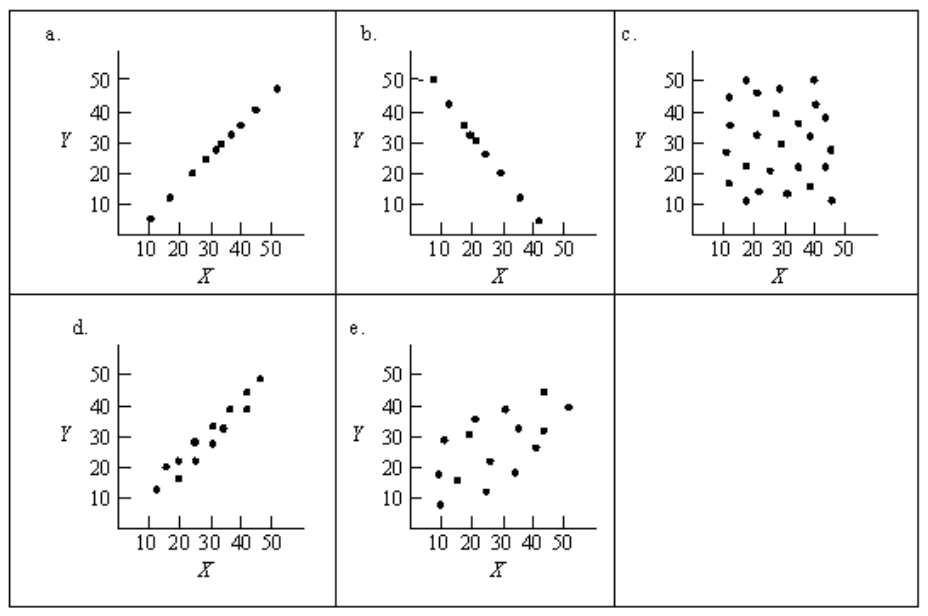
\includegraphics[width=0.8\linewidth]{figure/bra-scatterplots} \end{center}

\begin{enumerate}
\def\labelenumi{\arabic{enumi}.}
\setcounter{enumi}{3}
\tightlist
\item
  A correlation of about .60?

  \begin{enumerate}
  \def\labelenumii{\alph{enumii}.}
  \tightlist
  \item
    a
  \item
    b
  \item
    c
  \item
    d
  \item
    e
  \end{enumerate}
\item
  The strongest relationship between the \(X\) and \(Y\) variables?

  \begin{enumerate}
  \def\labelenumii{\alph{enumii}.}
  \tightlist
  \item
    a
  \item
    b
  \item
    a and b
  \item
    a and d
  \item
    a, b, and d
  \end{enumerate}
\end{enumerate}

\noindent Dr.~Jones gave students in her class a pretest about statistical concepts. After teaching about hypotheses tests, she then gave them a posttest about statistical concepts. Dr.~Jones is interested in determining if there is a relationship between pretest and posttest scores, so she constructed the following scatterplot and calculated the correlation coefficient.

\begin{center}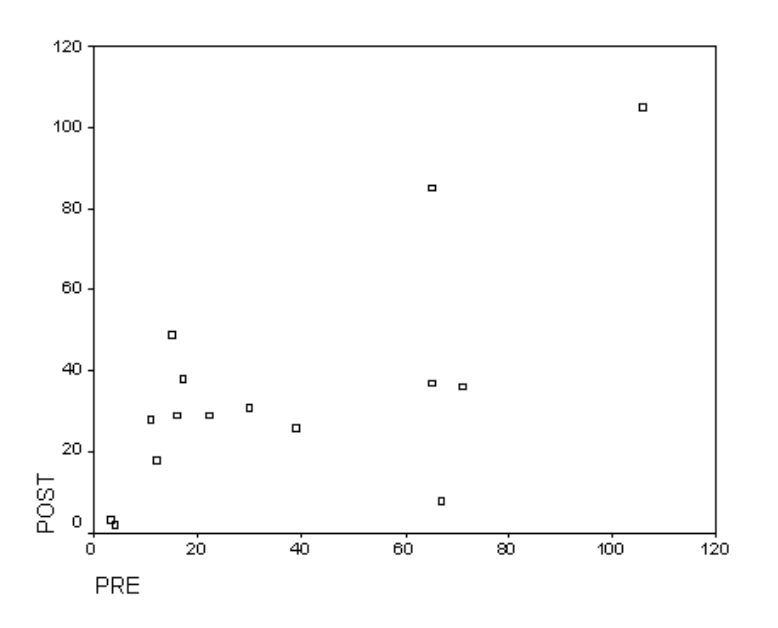
\includegraphics[width=0.6\linewidth]{figure/dr-jones-scatterplot} \end{center}

\begin{enumerate}
\def\labelenumi{\arabic{enumi}.}
\setcounter{enumi}{5}
\tightlist
\item
  Locate the point that shows a pretest score of 107. This point, which represents John's scores, is actually incorrect. If John's scores are removed from the data set, how would the correlation coefficient be affected?

  \begin{enumerate}
  \def\labelenumii{\alph{enumii}.}
  \tightlist
  \item
    The value of the correlation would decrease.
  \item
    The value of the correlation would increase.
  \item
    The value of the correlation would stay the same.
  \end{enumerate}
\item
  It turns out that John's pretest score was actually 5, and his posttest score was 100. If this correction is made to the data file and a new correlation coefficient is calculated, how would you expect this correlation to compare to the original correlation?

  \begin{enumerate}
  \def\labelenumii{\alph{enumii}.}
  \tightlist
  \item
    The absolute value of the new correlation would be smaller than the absolute value of the original correlation.
  \item
    The absolute value of the new correlation would be larger than the absolute value of the original correlation.
  \item
    The absolute value of the new correlation would be the same as the absolute value of the original correlation.
  \item
    It is impossible to predict how the correlation would change.
  \end{enumerate}
\item
  A statistics instructor wants to use the number of hours studied to predict exam scores in his class. He wants to use a linear regression model. Data from previous years shows that the average number of hours studying for a final exam in statistics is 8.5, with a standard deviation of 1.5, and the average exam score is 75, with a standard deviation of 15. The correlation is .76. Should the instructor use linear regression to predict exam scores from hours studied?

  \begin{enumerate}
  \def\labelenumii{\alph{enumii}.}
  \tightlist
  \item
    Yes, there is a high correlation, so it is alright to use linear regression.
  \item
    Yes, because linear regression is the statistical method used to make predictions when you have bivariate quantitative data.
  \item
    Linear regression could be appropriate if the scatterplot shows a clear linear relationship.
  \item
    No, because there is no way to prove that more hours of study causes higher exam scores.
  \end{enumerate}
\end{enumerate}

\hypertarget{distributional-reasoning-scale-drs}{%
\section*{Distributional Reasoning Scale (DRS)}\label{distributional-reasoning-scale-drs}}
\addcontentsline{toc}{section}{Distributional Reasoning Scale (DRS)}

Items 1 and 2 refer to the four histograms displayed below. For each item, match the description to the appropriate histogram.

\begin{center}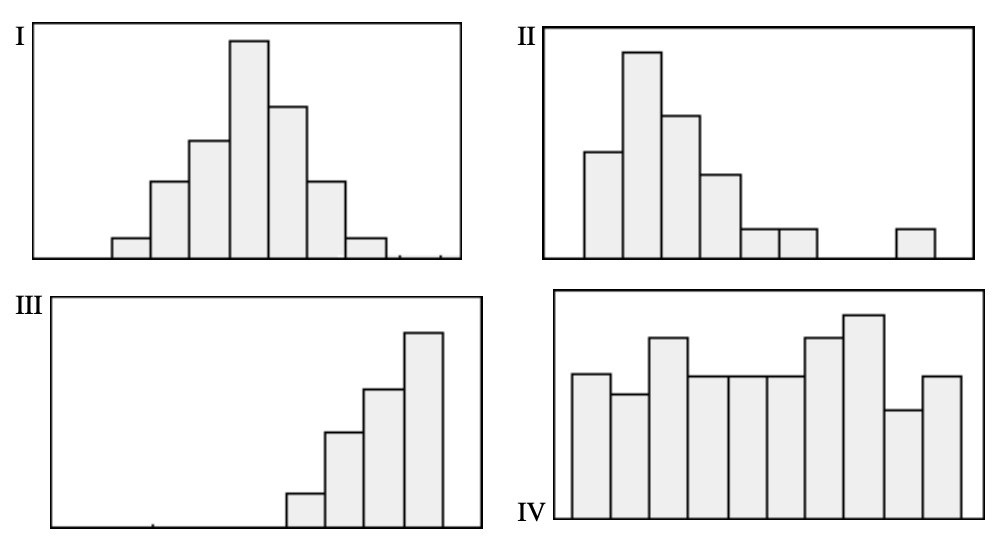
\includegraphics[width=0.8\linewidth]{figure/drs-01} \end{center}

\begin{enumerate}
\def\labelenumi{\arabic{enumi}.}
\tightlist
\item
  A distribution for a set of quiz scores where the quiz was very easy is represented by:

  \begin{enumerate}
  \def\labelenumii{\alph{enumii}.}
  \tightlist
  \item
    Histogram I
  \item
    Histogram II
  \item
    Histogram III
  \item
    Histogram IV
  \end{enumerate}
\item
  A distribution for the last digit of phone numbers sampled from a phone book (i.e., for the phone number 968-9667, the last digit, 7, would be selected) is represented by:

  \begin{enumerate}
  \def\labelenumii{\alph{enumii}.}
  \tightlist
  \item
    Histogram I
  \item
    Histogram II
  \item
    Histogram III
  \item
    Histogram IV
  \end{enumerate}
\item
  A baseball fan likes to keep track of statistics for the local high school baseball team. One of the statistics she recorded is the proportion of hits obtained by each player based on the number of times at bat as shown in the table below. Which of the following graphs gives the best display of the distribution of proportion of hits in that it allows the baseball fan to describe the shape, center and spread of the data?
\end{enumerate}

\begingroup\fontsize{10}{12}\selectfont

\begin{tabu} to \linewidth {>{\centering}X>{\centering}X>{\centering}X>{\centering}X>{\centering}X>{\centering}X}
\toprule
\multicolumn{1}{c}{Player} & \multicolumn{1}{c}{Prop} & \multicolumn{1}{c}{Player} & \multicolumn{1}{c}{Prop} & \multicolumn{1}{c}{Player} & \multicolumn{1}{c}{Prop}\\
\midrule
BH & 0.305 & SU & 0.270 & BC & 0.301\\
HA & 0.229 & DH & 0.136 & AA & 0.143\\
JS & 0.281 & TO & 0.218 & HK & 0.341\\
TC & 0.097 & RL & 0.267 & RS & 0.261\\
MM & 0.167 & JB & 0.270 & CR & 0.115\\
\addlinespace
GV & 0.333 & WG & 0.054 & MD & 0.125\\
RC & 0.085 & MH & 0.108 &  & NA\\
\bottomrule
\end{tabu}
\endgroup{}

\begin{center}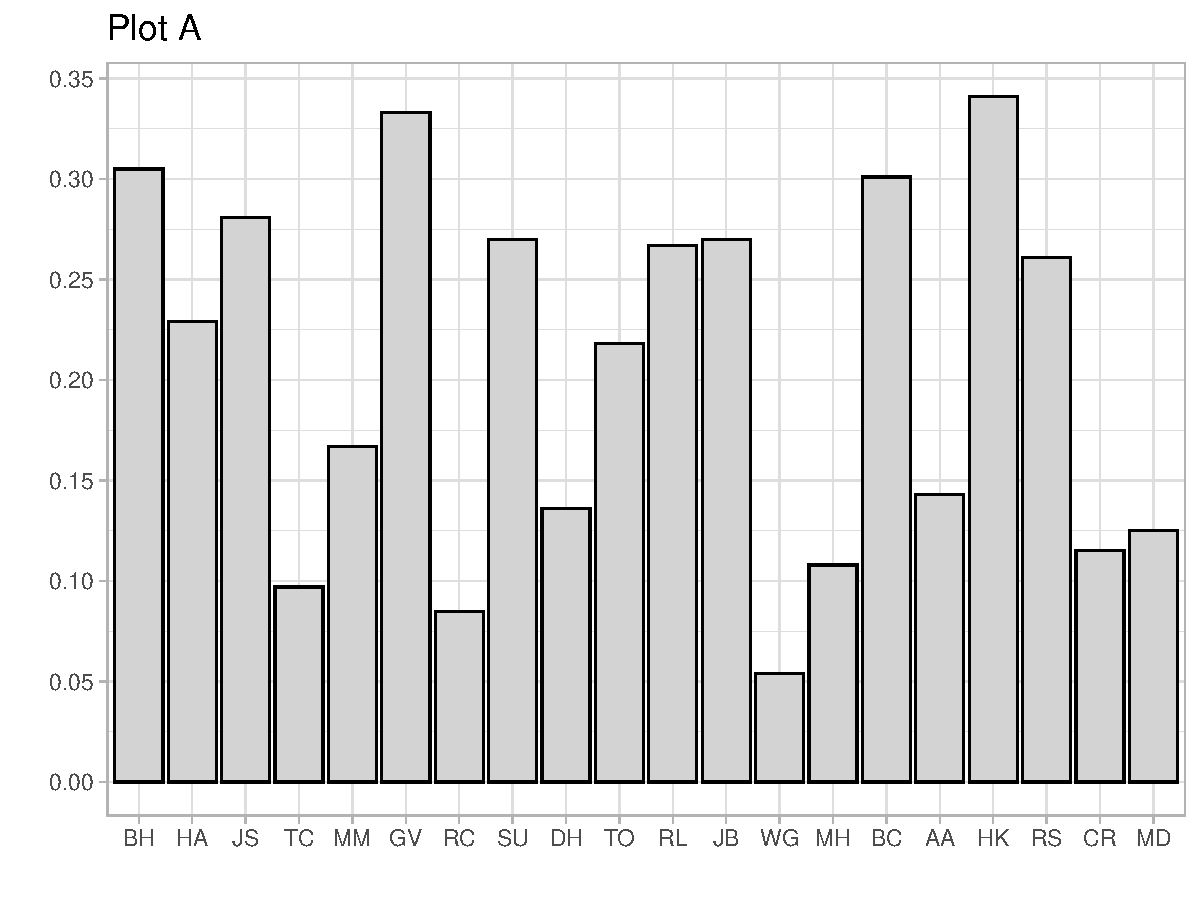
\includegraphics[width=0.6\linewidth]{thesis_files/figure-latex/fig-baseball-1} 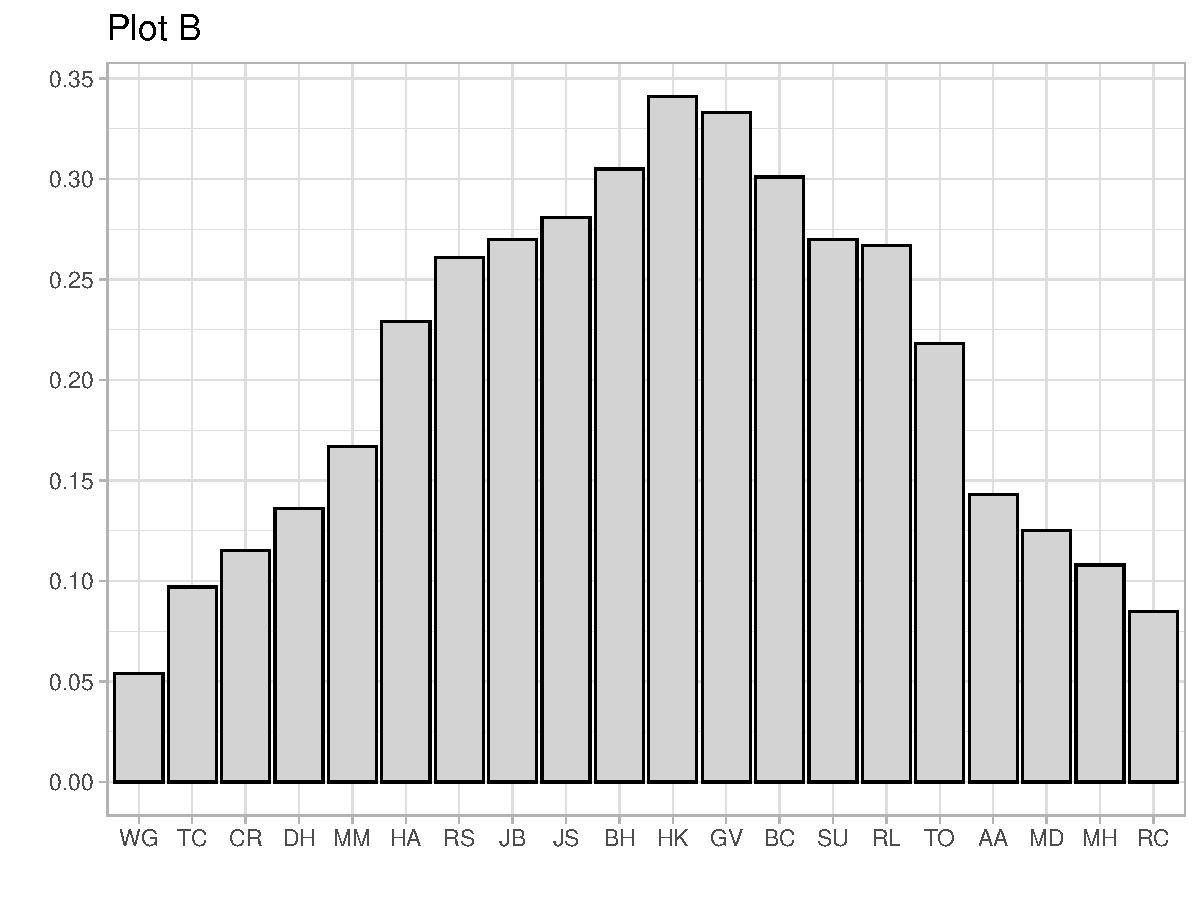
\includegraphics[width=0.6\linewidth]{thesis_files/figure-latex/fig-baseball-2} 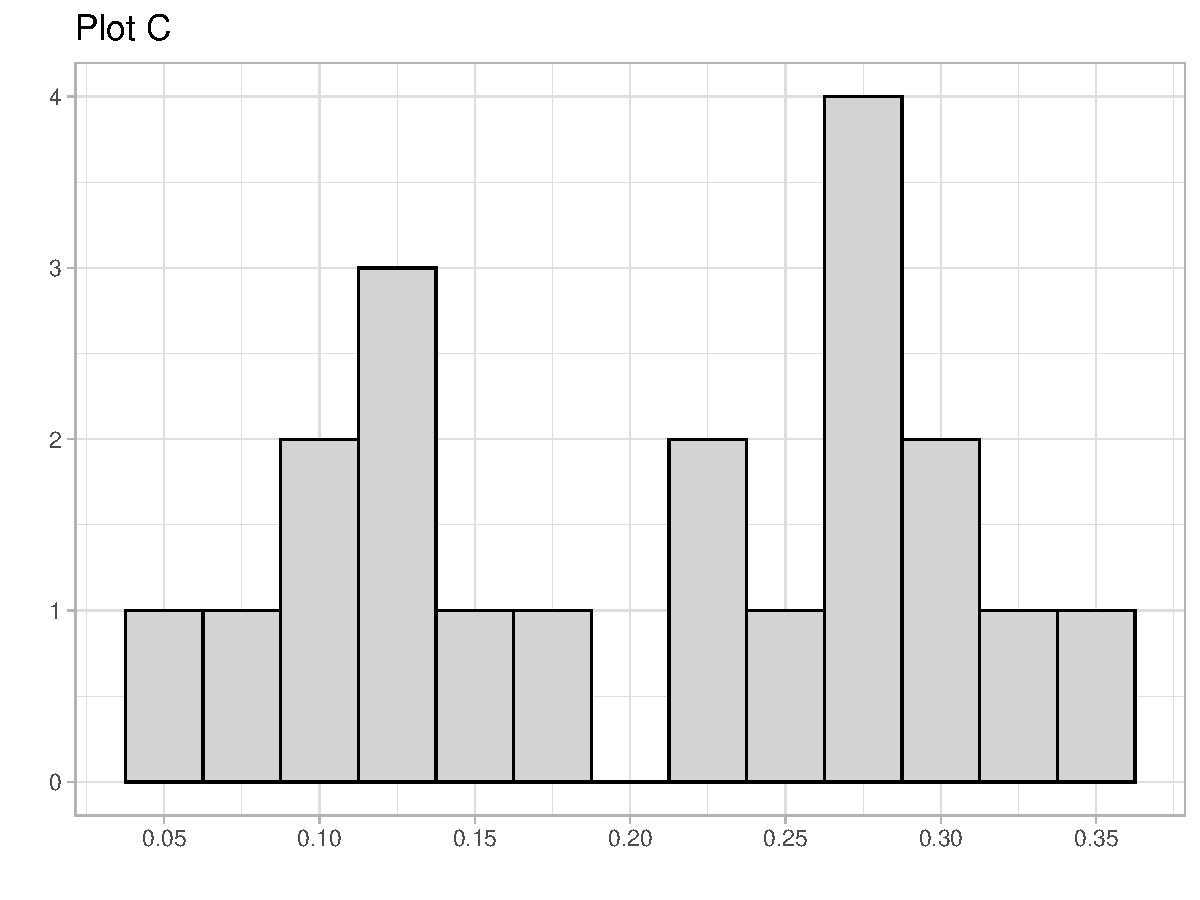
\includegraphics[width=0.6\linewidth]{thesis_files/figure-latex/fig-baseball-3} 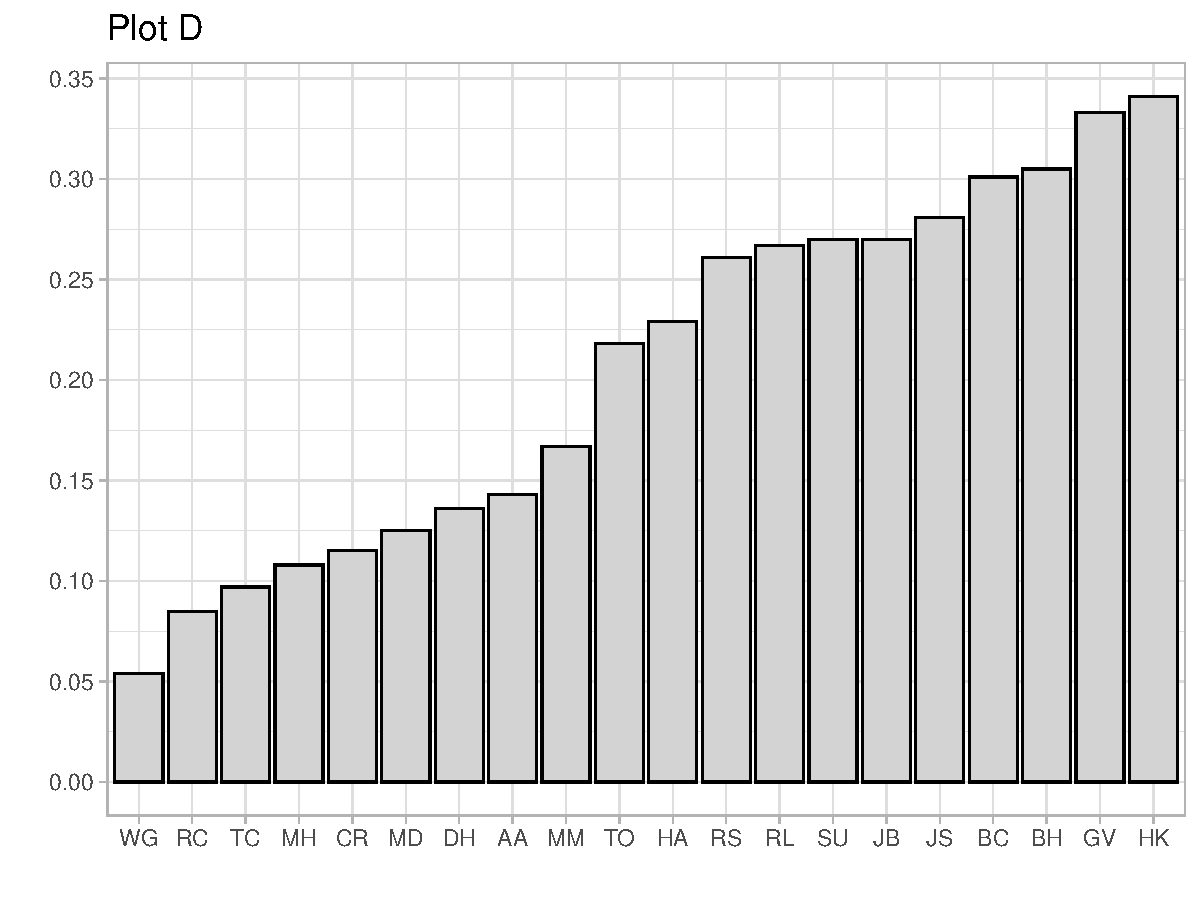
\includegraphics[width=0.6\linewidth]{thesis_files/figure-latex/fig-baseball-4} \end{center}

\noindent A drug company developed a new formula for their headache medication. To test the effectiveness of this new formula, they gave it to 100 people with headaches and timed how many minutes it took for the patient to no longer have a headache. They compared the result from this test to previous results from 150 patients using the old formula under the exact same conditions. The results from both of these clinical trials are shown below.

\begin{center}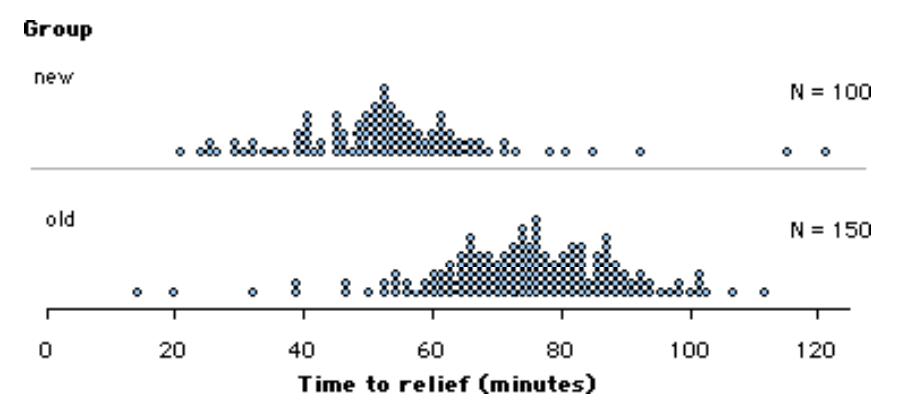
\includegraphics[width=0.8\linewidth]{figure/drs-04} \end{center}

\noindent Items 4, 5, and 6 present statements made by three different statistics students. For each statement, indicate whether you think the student's conclusion is valid.

\begin{enumerate}
\def\labelenumi{\arabic{enumi}.}
\setcounter{enumi}{3}
\tightlist
\item
  The old formula works better. Two people who took the old formula felt relief in less than 20 minutes, compared to none who took the new formula. Also, the worst result---near 120 minutes---was with the new formula.

  \begin{enumerate}
  \def\labelenumii{\alph{enumii}.}
  \tightlist
  \item
    Valid
  \item
    Invalid
  \end{enumerate}
\item
  The average time for the new formula is lower than the average time for the old formula. I'd conclude that people taking the new formula will tend to feel relief about 20 minutes sooner than those taking the old formula.

  \begin{enumerate}
  \def\labelenumii{\alph{enumii}.}
  \tightlist
  \item
    Valid
  \item
    Invalid
  \end{enumerate}
\item
  I wouldn't conclude anything from these data. The number of patients in the two groups is not the same so there is no fair way to compare the two formulas.

  \begin{enumerate}
  \def\labelenumii{\alph{enumii}.}
  \tightlist
  \item
    Valid
  \item
    Invalid
  \end{enumerate}
\end{enumerate}

\noindent Item 7 refers to the two boxplots presented below. The boxplots display final exam scores for all students in two different sections of the same course.

\begin{center}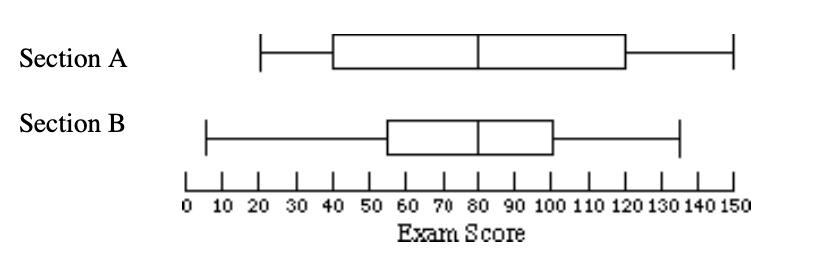
\includegraphics[width=0.8\linewidth]{figure/drs-07} \end{center}

\begin{enumerate}
\def\labelenumi{\arabic{enumi}.}
\setcounter{enumi}{6}
\item
  Which section would you expect to have a greater standard deviation in exam scores?

  \begin{enumerate}
  \def\labelenumii{\alph{enumii}.}
  \tightlist
  \item
    Section A
  \item
    Section B
  \item
    Both Sections are about equal
  \item
    It is impossible to tell
  \end{enumerate}
\item
  Jean lives about 10 miles from the college where she plans to attend a 10-week summer class. There are two main routes she can take to the school, one through the city and one through the countryside. The city route is shorter in miles, but has more stoplights. The country route is longer in miles, but has only a few stop signs and stoplights. Jean sets up a randomized experiment where each day she tosses a coin to decide which route to take that day. She records the following times in minutes for 5 days of travel on each route.

  \begin{itemize}
  \tightlist
  \item
    Country Route: 17, 15, 17, 16, 18
  \item
    City Route: 18, 13, 20, 10, 16
  \end{itemize}
\end{enumerate}

It is important to Jean to arrive on time for her class, but she does not want to arrive too early because that would increase parking fees. Based on the data gathered, which route would you advise her to choose?

\begin{enumerate}
\def\labelenumi{\alph{enumi}.}
\tightlist
\item
  The Country Route, because the times are consistently between 15 and 18 minutes.
\item
  The City Route, because she can get there in 10 minutes on a good day and the average time is less than for the Country Route.
\item
  Because times on the two routes have so much overlap, neither route is better than the other. She might as well flip a coin.
\end{enumerate}

\noindent Items 9 and 10 refer to the five histograms presented below. Each histogram displays test scores on a scale of 0 to 10 for one of five different statistics classes.

\begin{center}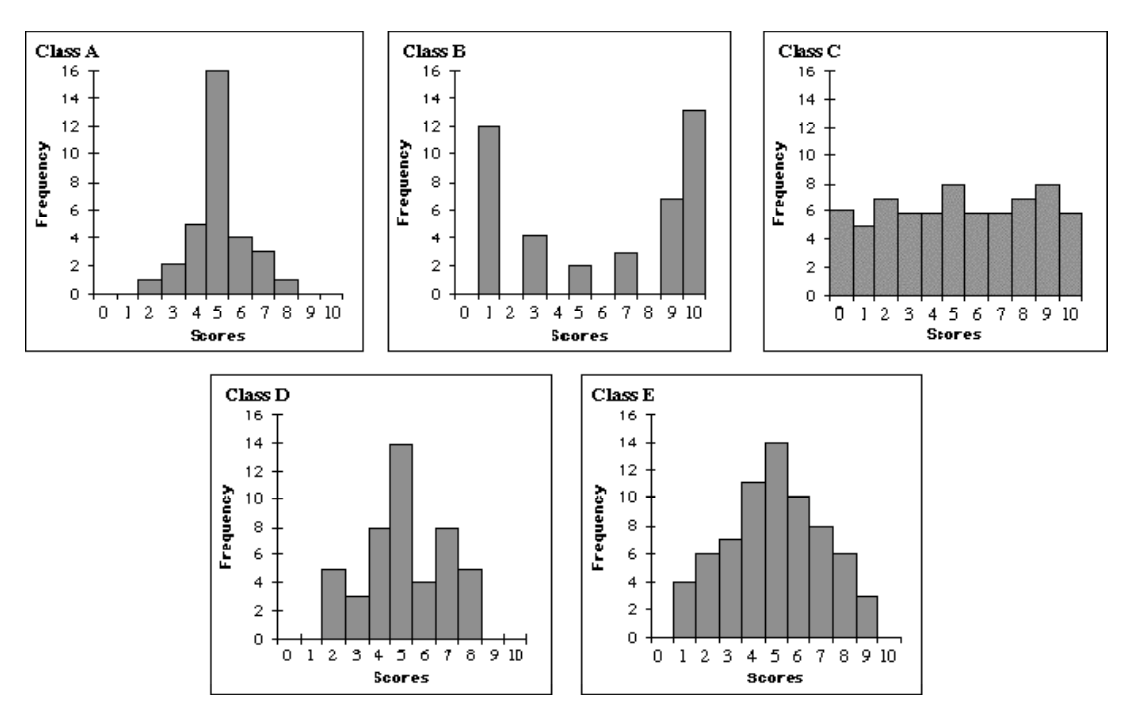
\includegraphics[width=0.8\linewidth]{figure/drs-09} \end{center}

\begin{enumerate}
\def\labelenumi{\arabic{enumi}.}
\setcounter{enumi}{8}
\tightlist
\item
  Which of the classes would you expect to have the lowest standard deviation, and why?

  \begin{enumerate}
  \def\labelenumii{\alph{enumii}.}
  \tightlist
  \item
    Class A, because it has the most values close to the mean.
  \item
    Class B, because it has the smallest number of distinct scores.
  \item
    Class C, because there is no change in scores.
  \item
    Class A and Class D, because they both have the smallest range.
  \item
    Class E, because it looks the most normal.
  \end{enumerate}
\item
  Which of the classes would you expect to have the highest standard deviation, and why?

  \begin{enumerate}
  \def\labelenumii{\alph{enumii}.}
  \tightlist
  \item
    Class A, because it has the largest difference between the heights of the bars.
  \item
    Class B, because more of its scores are far from the mean.
  \item
    Class C, because it has the largest number of different scores.
  \item
    Class D, because the distribution is very bumpy and irregular.
  \item
    Class E, because it has a large range and looks normal.
  \end{enumerate}
\end{enumerate}

\hypertarget{algebra-test-timss-study}{%
\section*{Algebra Test (TIMSS Study)}\label{algebra-test-timss-study}}
\addcontentsline{toc}{section}{Algebra Test (TIMSS Study)}

\begin{enumerate}
\def\labelenumi{\arabic{enumi}.}
\tightlist
\item
  The cost C, of printing greeting cards consists of a fixed charge of 100 cents and a charge of 6 cents for each card printed. Which of these equations can be used to determine the cost of printing \emph{n} cards?

  \begin{enumerate}
  \def\labelenumii{\alph{enumii}.}
  \tightlist
  \item
    \(C = (100 + 6n)\) cents
  \item
    \(C = (106 + n)\) cents
  \item
    \(C = (6 + 100n)\) cents
  \item
    \(C = (106n)\) cents
  \item
    \(C = (600n)\) cents
  \end{enumerate}
\item
  The table shows a relationship between \emph{x} and \emph{y}. Write an equation that expresses this relationship.
\end{enumerate}

\begin{longtable}[]{@{}ll@{}}
\toprule
\emph{x} & \emph{y} \\
\midrule
\endhead
2 & 7 \\
3 & 10 \\
4 & 13 \\
5 & 16 \\
\bottomrule
\end{longtable}

\hspace{2in}

Answer: y = \underline{\hspace{3cm}}

\pagebreak

\begin{enumerate}
\def\labelenumi{\arabic{enumi}.}
\setcounter{enumi}{2}
\tightlist
\item
  The table shows a relationship between \emph{x} and \emph{y}. What is the missing number in the table?
\end{enumerate}

\begin{enumerate}
\def\labelenumi{\alph{enumi}.}
\tightlist
\item
  9
\item
  10
\item
  11
\item
  12
\item
  13
\end{enumerate}

\begin{longtable}[]{@{}ll@{}}
\toprule
\emph{x} & \emph{y} \\
\midrule
\endhead
2 & 5 \\
3 & 7 \\
4 & ? \\
7 & 15 \\
\bottomrule
\end{longtable}

\begin{enumerate}
\def\labelenumi{\arabic{enumi}.}
\setcounter{enumi}{3}
\item
  Find the value of \emph{x} if: \(12x - 10 = 6x + 32\).
\item
  If 4 times a number is 48, what is \(\frac{1}{3}\) of the number?

  \begin{enumerate}
  \def\labelenumii{\alph{enumii}.}
  \tightlist
  \item
    4
  \item
    8
  \item
    12
  \item
    16
  \end{enumerate}
\item
  If \(x=3\), what is the value of \(\frac{5x + 3}{4x - 3}\)?
\item
  Which point on the graph could have coordinates \((7,~16)\)?

  \begin{enumerate}
  \def\labelenumii{\alph{enumii}.}
  \tightlist
  \item
    Point P
  \item
    Point Q
  \item
    Point R
  \item
    Point S
  \end{enumerate}
\end{enumerate}

\begin{center}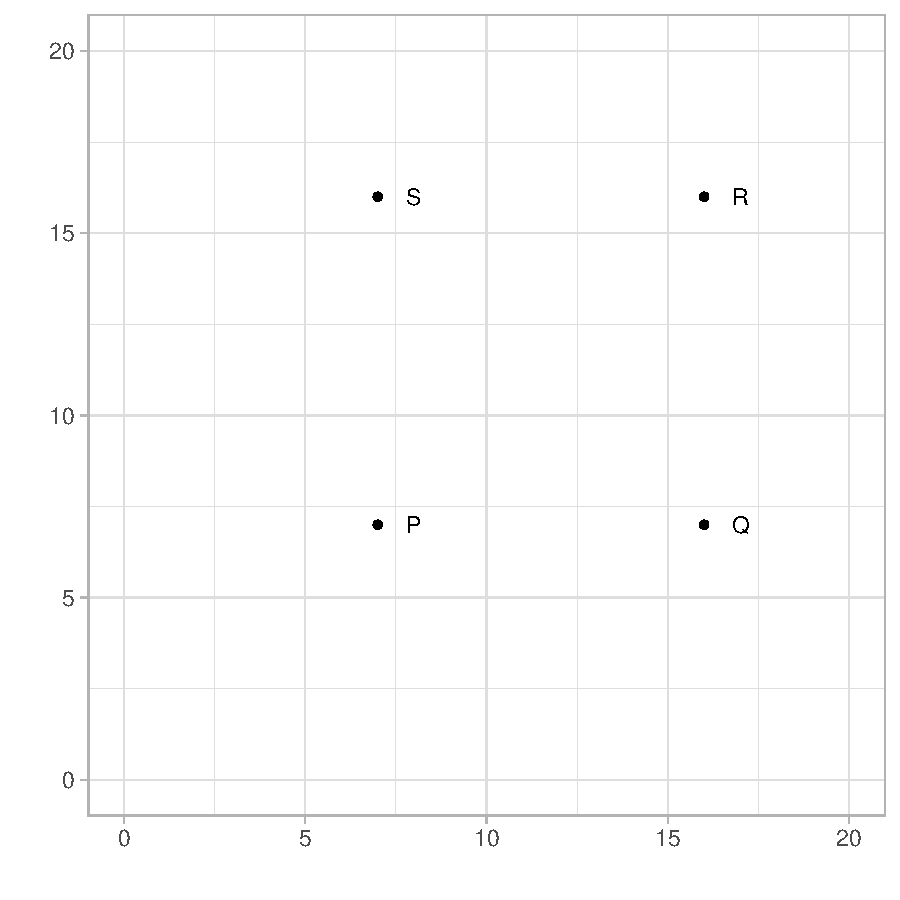
\includegraphics[width=0.6\linewidth]{thesis_files/figure-latex/fig-algtest-07-1} \end{center}

\begin{enumerate}
\def\labelenumi{\arabic{enumi}.}
\setcounter{enumi}{7}
\item
  A club has 86 members, and there are 14 more girls than boys. How many boys and how many girls are members of the club? \emph{Show your work.}
\item
  The table shows some values of \emph{x} and \emph{y}, where \emph{x} is proportional to \emph{y}. What are the values of \emph{P} and \emph{Q}?

  \begin{enumerate}
  \def\labelenumii{\alph{enumii}.}
  \tightlist
  \item
    \(P=40\) and \(Q=13\)
  \item
    \(P=18\) and \(Q=17\)
  \item
    \(P=20\) and \(Q=18\)
  \item
    \(P=40\) and \(Q=18\)
  \item
    \(P=18\) and \(Q=20\)
  \end{enumerate}
\end{enumerate}

\begin{longtable}[]{@{}ll@{}}
\toprule
\emph{x} & \emph{y} \\
\midrule
\endhead
4 & 9 \\
8 & \emph{P} \\
\emph{Q} & 45 \\
\bottomrule
\end{longtable}

\begin{enumerate}
\def\labelenumi{\arabic{enumi}.}
\setcounter{enumi}{9}
\tightlist
\item
  Solve the equation for \emph{x}. Show your work.
\end{enumerate}

\[
x^2 - 11x + 10 = 0
\]

\hypertarget{mathematics-background-questionnaire-naep-items}{%
\section*{Mathematics Background Questionnaire (NAEP Items)}\label{mathematics-background-questionnaire-naep-items}}
\addcontentsline{toc}{section}{Mathematics Background Questionnaire (NAEP Items)}

Which courses have you taken during high school or college? \textbf{Check one or box on each line.} INCLUDE courses taken in summer school, but DO NOT INCLUDE topics that were only taught as part of a longer course (such as trigonometry taught in drafting class or computer programming taught in Algebra II). If you have taken \textbf{more than one course at a particular level} (e.g., you took two statistics courses in college) please indicate how many you have taken along with the check mark.

\begingroup\fontsize{10}{12}\selectfont
\setlength{\LTleft}{0pt}
\begin{longtable}[t]{|>{\raggedright\arraybackslash}p{2in}|>{\centering\arraybackslash}p{0.75in}|>{\centering\arraybackslash}p{0.75in}|>{\centering\arraybackslash}p{0.75in}|>{\centering\arraybackslash}p{0.75in}|}
\toprule
\thead{} & \thead{Never} & \thead{High school} & \thead{College} & \thead{Both}\\
\midrule
\endfirsthead

\toprule
\thead{} & \thead{I have never\\ taken this\\ course.} & \thead{I took this\\ course in high\\ school.} & \thead{I took this\\ course in\\ college.} & \thead{I took this\\ course in both\\ high school\\ and college.}\\
\midrule
\endhead
\bottomrule

\endfoot
\bottomrule
\endlastfoot
Basic or general mathematics course &  &  &  & \\
\midrule
Tech-prep mathematics course &  &  &  & \\
\midrule
Pre-algebra course &  &  &  & \\
\midrule
Algebra I course &  &  &  & \\
\midrule
Geometry course &  &  &  & \\
\midrule
Algebra II course, with trigonometry &  &  &  & \\
\midrule
Algebra II course, w/o trigonometry &  &  &  & \\
\midrule
Trigonometry (as a separate course) &  &  &  & \\
\midrule
Pre-calculus course &  &  &  & \\
\midrule
Integrated mathematics course &  &  &  & \\
\midrule
Probability or statistics course &  &  &  & \\
\midrule
Calculus course &  &  &  & \\
\midrule
Discrete mathematics course &  &  &  & \\
\midrule
Other mathematics course &  &  &  & \\
\midrule
Computer programming course (such as C++, Pascal, Visual Basic, etc.) &  &  &  & \\*
\end{longtable}
\endgroup{}

\hypertarget{appendix-b}{%
\chapter{Consent Form}\label{appendix-b}}

\emph{The Effectiveness of Multiple Learning Tools and Activities in Helping Students Learn Statistics}

\noindent You are invited to be in a research study on the effectiveness of different learning tools and activities to help students learn statistics. You were selected as a possible participant because you are enrolled in EPSY 3264. We ask that you read this form and ask any questions you may have before agreeing to be in the study.

\noindent This study is being conducted by: Andrew Zieffler, Educational Psychology, EPSY 3264 Instructor

\noindent \textbf{Background Information:} The purpose of this study is: to study the effectiveness of different learning tools and activities to help students learn statistics. The specific research question to be answered is: What learning tools and activities seem to help students learn statistics best?

\noindent \textbf{Procedures:} If you agree to be in this study, we would ask you to do the following things:

\begin{enumerate}
\def\labelenumi{(\arabic{enumi})}
\tightlist
\item
  Take a 20 question test two times during the semester. These two test scores will not be used to determine your grade. They are extra credit opportunities only. Each test will take approximately 20--25 minutes to complete
\item
  Provide consent to the University of Minnesota to release your overall ACT score once the semester has been completed. The ACT score will be added to the data file (being used by the researcher) by the Office of Institutional Research and Reporting. Once the ACT score has been added to the data file, all personal identification (names and ID numbers) will be erased and the file will be randomly sorted so the researcher will not know the identity of the student.
\end{enumerate}

\noindent \textit{Note:} If you don't want your ACT score released, but still want to participate in the study by taking the tests, that is all right.

\noindent \textbf{Risks and Benefits of being in the Study:} The study has minimal risks. There are no benefits to being involved in the study.

\noindent \textbf{Compensation:}\} You will receive payment: You will receive class points equivalent to one quiz for each of the optional tests you complete. For instance, if you take both optional tests then you will receive class points equivalent to replace two of your quiz scores.

\noindent \textbf{Confidentiality:} The records of this study will be kept private. In any sort of report we might publish, we will not include any information that will make it possible to identify a subject. Research records will be stored securely and only researchers will have access to the records.

\noindent \textbf{Voluntary Nature of the Study:} Participation in this study is voluntary. Your decision whether or not to participate will not affect your current or future relations with the University of Minnesota. If you decide to participate, you are free to not answer any question or withdraw at any time with out affecting those relationships.

\noindent \textbf{Contacts and Questions:} The researcher conducting this study is: Andrew Zieffler. You may ask any questions you have now. If you have questions later, you are encouraged to contact him at 325 Burton Hall, 763-498-4392, \href{mailto:zief0002@umn.edu}{\nolinkurl{zief0002@umn.edu}}. (You can also contact Joan Garfield, 204 Burton Hall, 612-625-0337, \href{mailto:jbg@umn.edu}{\nolinkurl{jbg@umn.edu}})

\noindent If you have any questions or concerns regarding this study and would like to talk to someone other than the researcher(s), you are encouraged to contact the Research Subjects' Advocate Line, D528 Mayo, 420 Delaware St.~Southeast, Minneapolis, Minnesota 55455; (612) 625-1650.

\noindent You will be given a copy of this information to keep for your records.

\noindent \textbf{Statement of Consent:}

\noindent I have read the above information. I have asked questions and have received answers. I consent to participate in the study.

\noindent Signature: \underline{\hspace{3in}} Date: \underline{\hspace{1in}}

\noindent Signature of Investigator: \underline{\hspace{3in}} Date: \underline{\hspace{1in}}

\newpage

\hypertarget{act-score-release-form}{%
\section*{ACT Score Release Form}\label{act-score-release-form}}
\addcontentsline{toc}{section}{ACT Score Release Form}

As a part of the research study on the effectiveness of different learning tools and activities to help students learn statistics that you have agreed to be a participant in, we are asking that you consider providing the University of Minnesota consent to release your ACT score. We ask that you read this form and ask any questions you may have before agreeing to provide consent to release your ACT score.

\noindent If you agree to provide consent, you will be allowing the University of Minnesota to release your overall ACT score once the semester has been completed. The ACT score will be added to the data file (being used by the researcher) by the Office of Institutional Research and Reporting. Once the ACT score has been added to the data file, all personal identification (names and ID numbers) will be erased and the file will be randomly sorted so the researcher will not know the identity of the student.

\noindent We ask that if you agree to provide consent to the University of Minnesota to release your ACT score, that you do the following:

\begin{enumerate}
\def\labelenumi{(\arabic{enumi})}
\tightlist
\item
  Sign and date this form.
\item
  Mail this form to the address below, or drop this form off in Burton Hall 206 after grades
  have been submitted
\end{enumerate}

\noindent \hspace*{2in}

\begin{minipage}{.8\textwidth}
Andrew Zieffler \newline
Educational Psychology Room 107 BuH\newline
3171\newline
178 Pillsbury Dr. SE\newline
Minneapolis, MN 55455\newline
\end{minipage}

\noindent The records of this study will be kept private. In any sort of report we might publish, we will not include any information that will make it possible to identify a subject. Research records will be stored securely and only researchers will have access to the records.

\noindent The researcher conducting this study is: Andrew Zieffler. You may ask any questions you have now. If you have questions later, you are encouraged to contact him at 325 Burton Hall, 763-498-4392, \href{mailto:zief0002@umn.edu}{\nolinkurl{zief0002@umn.edu}}. (You can also contact Joan Garfield, 204 Burton Hall, 612-625-0337, \href{mailto:jbg@umn.edu}{\nolinkurl{jbg@umn.edu}}).

\noindent By signing this consent form, I am agreeing to allow the University of Minnesota to release my overall ACT score.

\noindent Signature: \underline{\hspace{3in}} Date: \underline{\hspace{1in}}

\noindent ID Number: \underline{\hspace{3in}}


\end{document}
